% !Mode:: "TeX:UTF-8"
% !TEX program  = xelatex
%\documentclass{cumcmthesis}
\documentclass[withoutpreface,bwprint]{cumcmthesis} %去掉封面与编号页,电子版提交的时候使用。
\usepackage{etoolbox}
\BeforeBeginEnvironment{tabular}{\zihao{-5}}
\usepackage{cite}
\usepackage[numbers,sort&compress]{natbib}
\usepackage[framemethod=TikZ]{mdframed}
\usepackage{url}   % 网页链接
\usepackage{subcaption} % 子标题
\title{基于方差/CVaR风险度量的投资组合优化}
\tihao{A}
\baominghao{4321}
\schoolname{华中科技大学}
\membera{ }
\memberb{ }
\memberc{ }
\supervisor{ }
\yearinput{2020}
\monthinput{08}
\dayinput{22}




\begin{document}
	
	\maketitle
		\begin{center}
		姓名:\underline{ 郑文斌 } 班级:\underline{ 光电1902 } 学号:\underline{ U201913935}
	\end{center}
	\begin{abstract}
		本文主要的问题有3个方面,分别是选取最具潜力股票、选取投资组合方案、确定方案的预期收益和风险。
		
		对于问题一的最具潜力股票的选取,本文通过附件中的数据,利用因子分析,将11个指标浓缩成3个因子,利用主成分分析的方法进行方差旋转,得到各个股票的因子得分,最后通过得分来评估股票的潜力,得分结果见表\ref{因子分析综合得分}。最终得到最具潜力的5只股票分别为贵州茅台、迈瑞医疗、英科医疗、片仔癀、海天味业。
		
		对于问题二、三,风险资产的投资首先需要解决的是两个核心问题:即预期收益与风险。 如何测定组合投资的风险与收益和如何平衡这两项指标进行资产分配也是投资者迫切需要解决的问题。
		
		本文首先建立的均值-方差模型是投资组合理论的基础,其以资产收益率的均值来反映投资收益,以收益率的方差来描述风险,是一个多目标规划问题。通过给定预期收益或者风险值,可以转化单目标规划,即最大收益模型、最小方差模型,同时,通过夏普比率的概念可以转化为最大夏普比率模型。
		
		CVaR 方法是近些年被广泛使用的风险测量方法。本文将CVaR 方法与均值-方差模型相结合,构建了均值-CVaR 模型,以CVaR 代替方差刻画了收益率时间序列的尾部风险的大小,并通过线性规划求解方法,通过选择不同的置信水平来控制风险,得到不同的投资组合有效前沿,并通过最大条件夏普比率计算出在不同置信水平下最优的投资组合权重。
		
		基于模型的要求,本文对各股票收益率进行了正态性检验,进而对模型求解,绘制了两主要模型的有效前沿,计算了各模型投资组合权重对应的预期年收益、风险,并对数据进行了汇总和对比分析,结果见表\ref{两模型投资组合比例及对应的收益风险汇总}。并以这些权重进行模拟投资,对一年内每天的收益进行累积,并增加一种等权重投资的对照组,绘制收益曲线,结果见图\ref{两模型求得的不同权重下的收益曲线}.
		
		
		\keywords{因子分析\quad  风险度量\quad   均值-方差模型 \quad  均值-CVAR模型 \quad 夏普比率 \quad 有效前沿}
	\end{abstract}
	
	%目录  2019 明确不要目录,我觉得这个规定太好了
	\tableofcontents
	
%	\newpage
	
	\section{问题重述}
	\subsection{问题背景}
	随着后疫情时代的到来,我国资本市场的发展和证券交易规模不断扩大,越 来越多的资金投资于证券市场,与此同时市场价格的波动也十分剧烈,而波动作 为证券市场中最本质的属性和特征。市场的波动对于人们风险收益的分析、股东权益最大化和监管层的有效监管都有着至关重要的作用,因此研究证券市场波动的规律性,分析引起市场波动的成因,是证券市场理论研究和实证分析的重要内容,也可以为投资者、监管者和上市公司等提供有迹可循的依据。
	
	\subsection{问题要求}
	1. 通过建立模型,请你从上述20支股票中,筛选出你认为最有潜力的5支股票。
	
	2.  有1亿元的初始资金,通过建立模型,请给出合理选股方案和投资组合方案。
	
	3.  给出合理的评价指标来评估你的上述投资策略的风险与预期年收益。
	
	\section{问题分析}
	本文主要的问题有3个方面,分别是选取最具潜力股票、选取投资组合方案、确定方案的预期收益和风险,需要根据附件20只股票数据来选取最具潜力股票和最佳的投资方案。对于投资组合方案的确定,可以通过建立组合优化模型来获取最佳的投资方案。
	
	为了方便看出股票近期的走势,需要首先对数据进行可视化分析,可以选取一只股票进行相关参数的定性分析,主要分析该股票的波动趋势以及数据的分布状况。另外再对所以股票的相关参数进行分析,以看出总体情况。
	
	对于问题一,可以采用因子分析的方法。因子分析主要是通过降维技术把多个变量化为少数几个主成分,构造出新的主成分方程,通过这些主成分来反映原始变量所包含的大部分信息。使用因子分析首先需要进行KMO检验和巴特利特球形检验,以检查数据是否适用因子分析。之后选择累计贡献率大于90\%的前若干个因子,计算因子载荷矩阵,并最终得到综合排名。
	
	对于问题二和问题三,一般来说, 风险资产的投资首先需要解决的是两个核心问题:即预期收益与风险。 如何测定组合投资的风险与收益和如何平衡这两项指标进行资产分配也是投资者迫切需要解决的问题。
	
	参考相关文献,发现可以从两个方面来评价投资的风险:一种是传统的方差,另一种是CVaR条件风险价值。本文参考马科维茨理论,建立了均值-方差模型和均值-CVaR模型。
	
	均值-方差模型和均值-CVaR模型本质上是多目标规划模型,即收益最大化、风险最小化,在给定收益或者风险的情况下,多目标规划可以转化为单目标规划,即风险最小模型和收益最大模型。通过相关方法求解可以得到两个模型的有效前沿。
	
	利用夏普比率或者条件夏普比率,可以在有效前沿中选择夏普比率最大时对应的投资组合比例,并计算这些模型对应的预期收益和风险,并对多个模型的结果进行对比分析。
		 \begin{figure}[H]
		\centering
		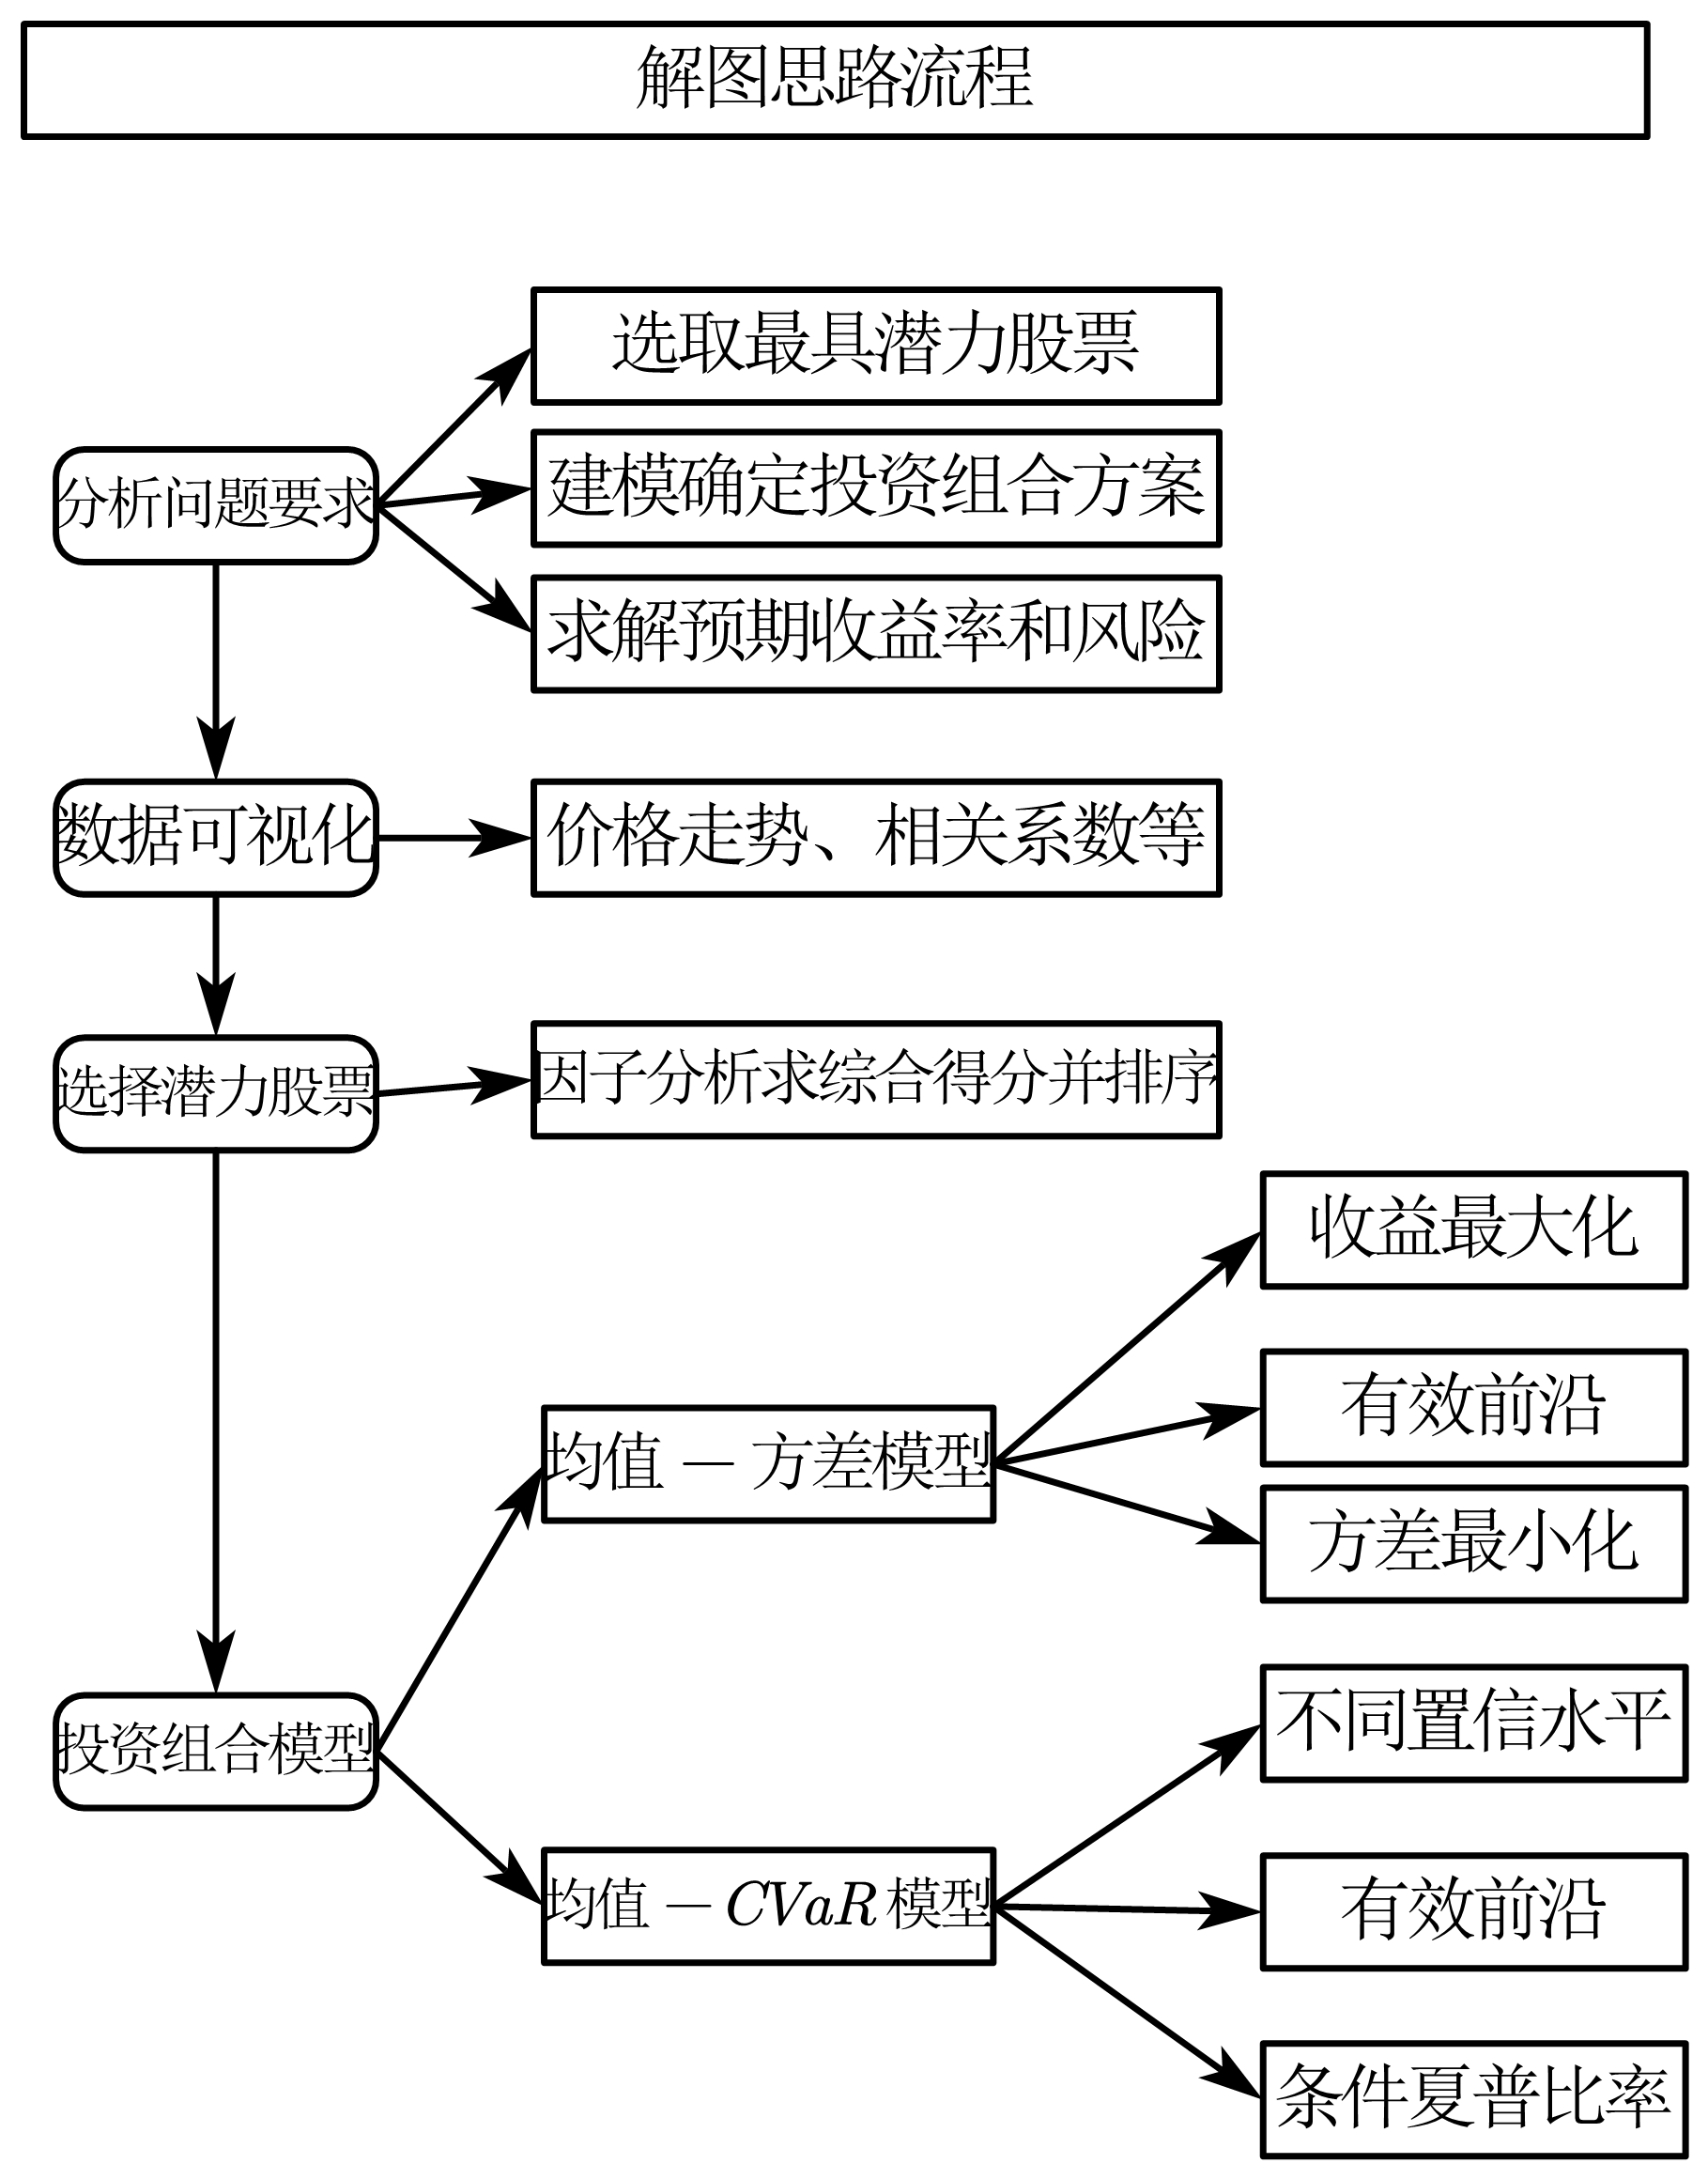
\includegraphics[width=0.6\textwidth]{流程图}
		\caption{解题流程图}
		\label{流程图}
	\end{figure}
	
	\section{模型假设}
	任何理论都是建立在一定的基本前提和理论假设之上的,本文的Markowitz 均值-方
	差模型和均值-CVaR模型也是如此,理论假设主要包括以下几个方面:
	
	
	②投资收益率的数学期望和方差或者CVaR可以比较全面的反映该投资的收益和风险状
	况;
	
	③投资者只关心预期收益和风险水平,忽略影响投资决策的影响因素;
	
	④投资者都是风险厌恶和不知足的,他们总希望收益率越高,风险越低越好;
	
	⑤市场信息是完全的,并且存在无风险资产,使得所有投资者对无风险资产
	和各种风险资产的收益率的预期都可以达成共识,投资者会在此基础上对给定的
	数据进行分析和决策。
	
	
	\section{符号说明}
	% Table generated by Excel2LaTeX from sheet 'Sheet1'
	\begin{table}[htbp]
		\centering
		\caption{本文主要符号说明}
		\begin{tabular}{ll}
			\toprule[1.5pt]
			符号    & 说明 \\
			\midrule
			$N     		$	& 股票的数量 \\
			$\mu_i   		$	& 第$i$个股票的收益率均值 \\
			$x_i    		$	& 投资在第$i$个股票的资本比例 \\
			$r     		$	& 投资组合的收益率 \\
			$R     		$	& 期望收益 \\
			$W_0   		$	& 投资者可承受的风险水平上限   \\
			$\Sigma   		$	& 各个股票之间的协方差矩阵 \\
			$\sigma_{ij}	$	& 协方差矩阵的项 \\
			$\sigma^2$ 		& 均值-方差模型投资组合的风险 \\
			$\lambda$ 			& 风险规避参数 \\
			$ERp   	$	& 投资组合预期收益 \\
			$R_f  		$	& 无风险资产收益 \\
			SharpeRatio 	& 夏普比率 \\
			Conditional SharpeRatio & 条件夏普比率 \\
			$\alpha$ & 1-置信水平 \\
			\bottomrule[1.5pt]
		\end{tabular}%
		\label{tab:addlabel}%
	\end{table}%
	
	
	\section{模型的建立和求解}
	
	\subsection{数据的可视化}
	\subsubsection{总体收盘价}
	附件一的成分股数据中包含了一共20支股票 我们首先针对所有20股票的相关走势
	进行分析 。我们首先给出20支股票的收盘价在一年内随着时间的变化趋势具体的走势如下:
	 \begin{figure}[H]
		\centering
		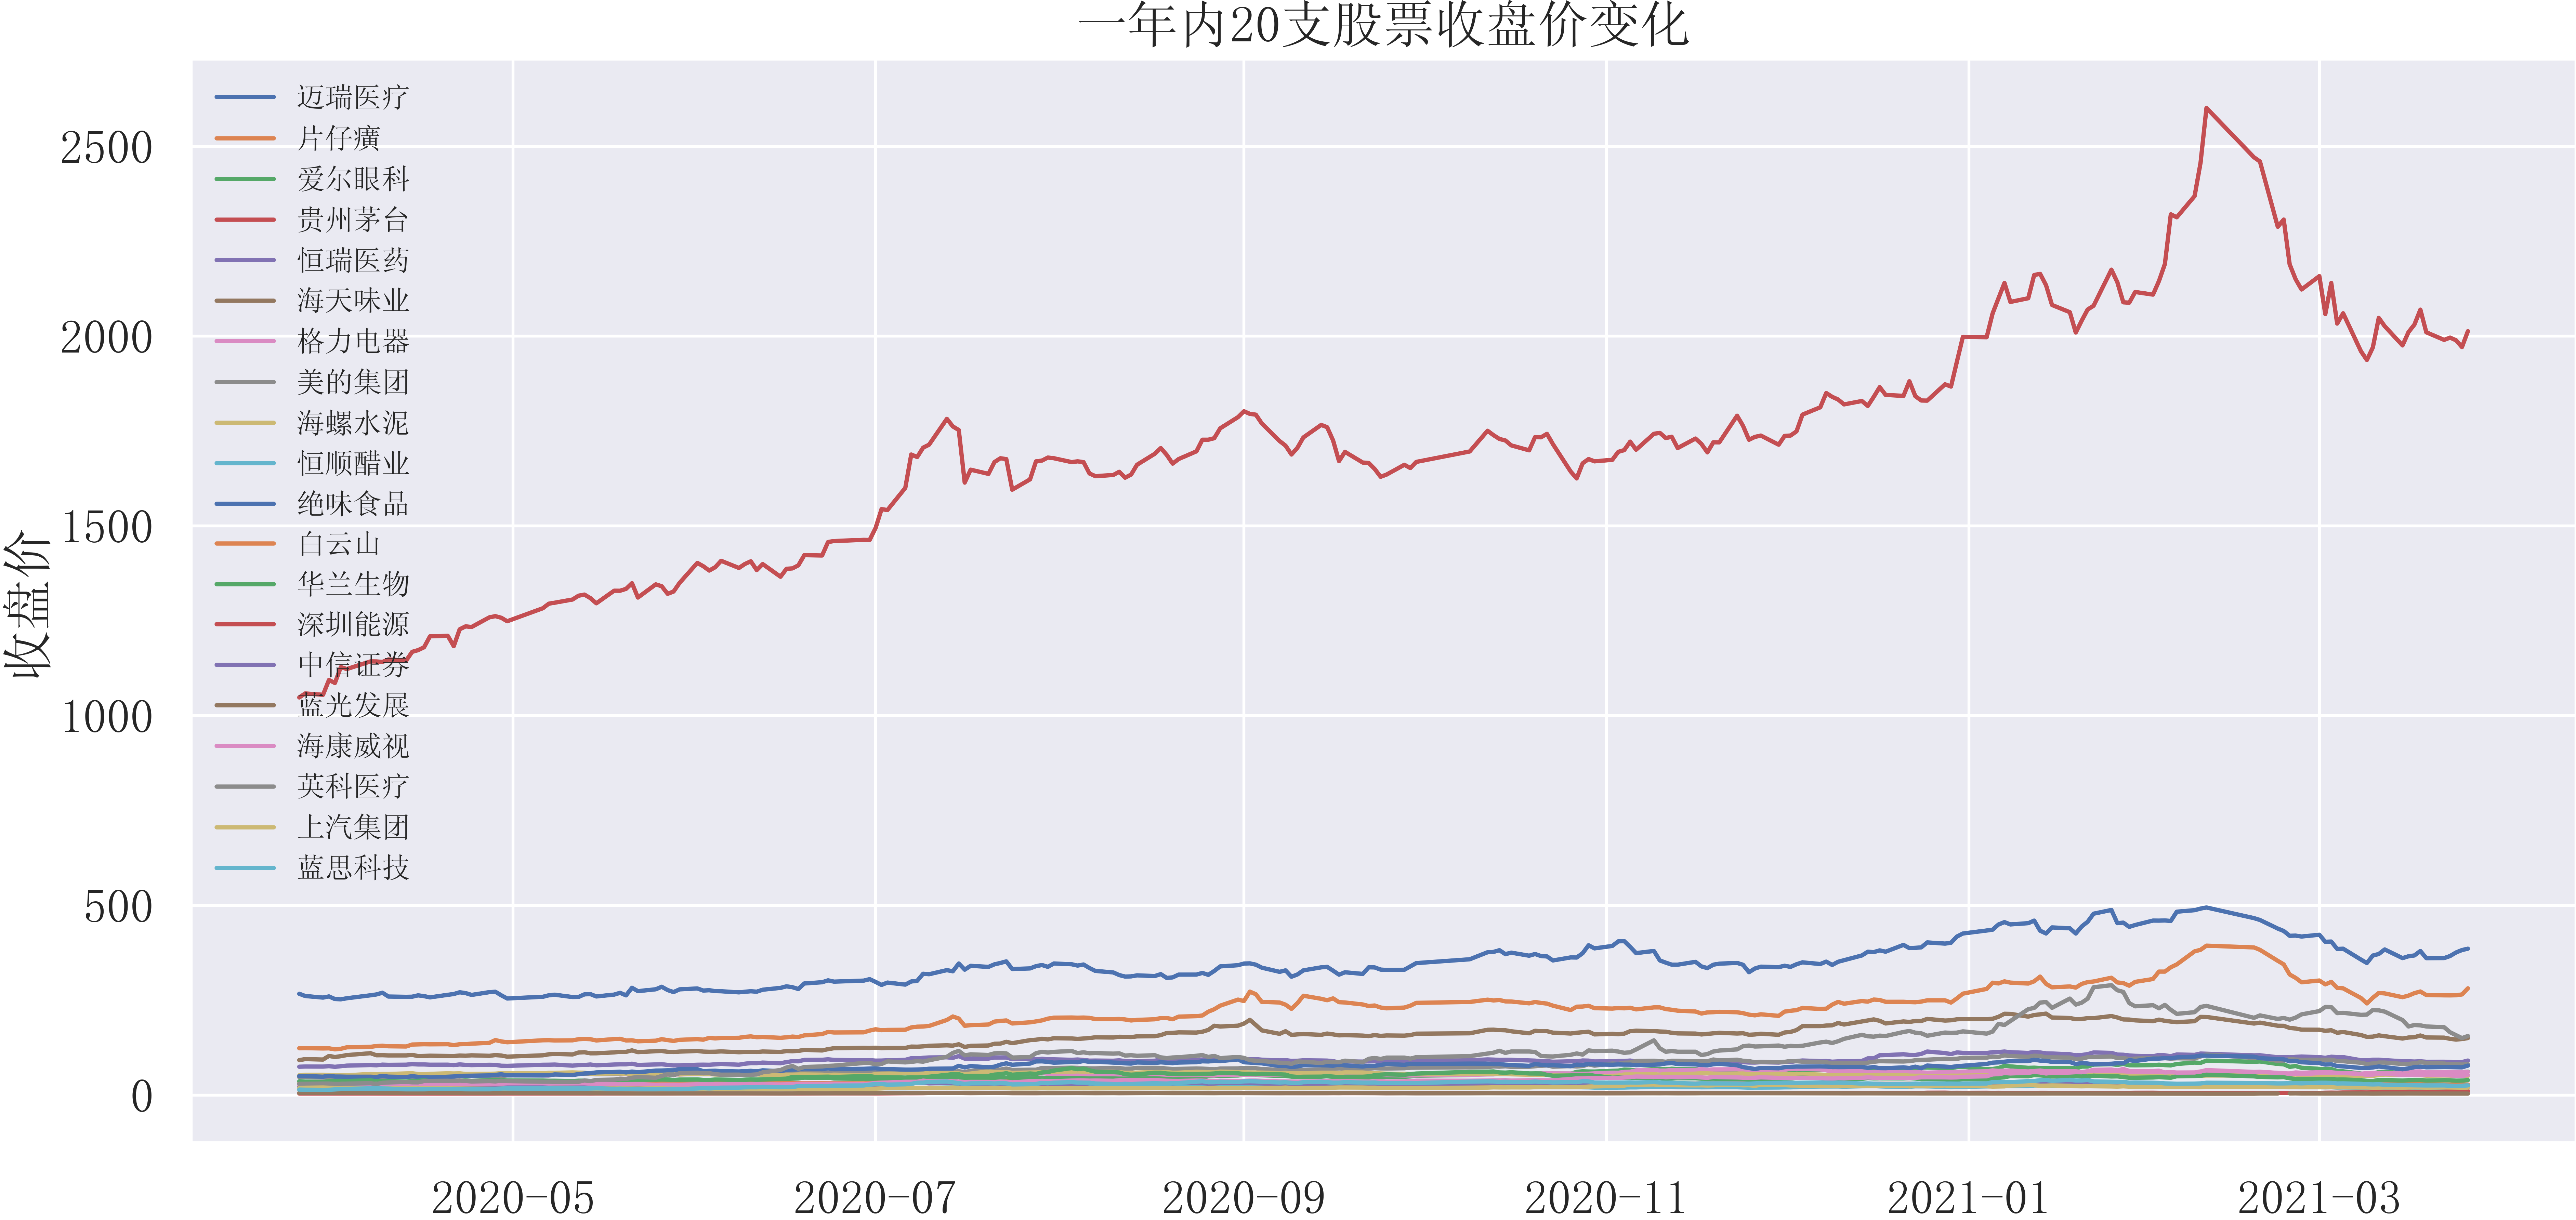
\includegraphics[width=0.8\textwidth]{一年内20支股票收盘价变化}
		\caption{一年内20支股票收盘价变化}
		\label{一年内20支股票收盘价变化}
	\end{figure}
根据上图我们可以得到各种股票走势基本一致 ,除贵州茅台外,其他股票的收盘价维持在较低水平,而贵州茅台的收盘价和其他股票相比差距很大。贵州茅台的股价相对于去年的股价整整翻了一倍多。这也说明了贵州茅台股价波动较大,风险水平较高,而其他19只股票虽然收益较低,但是波动较小,股票风险也比较小。因此我们后续的选股模型需要以此分析作为依据。充分考虑股票投资的收益与风险,从两个角度出发,做到两者兼顾的投资选股。
	\subsubsection{收盘价及成交额}
	 \begin{figure}[H]
		\centering
		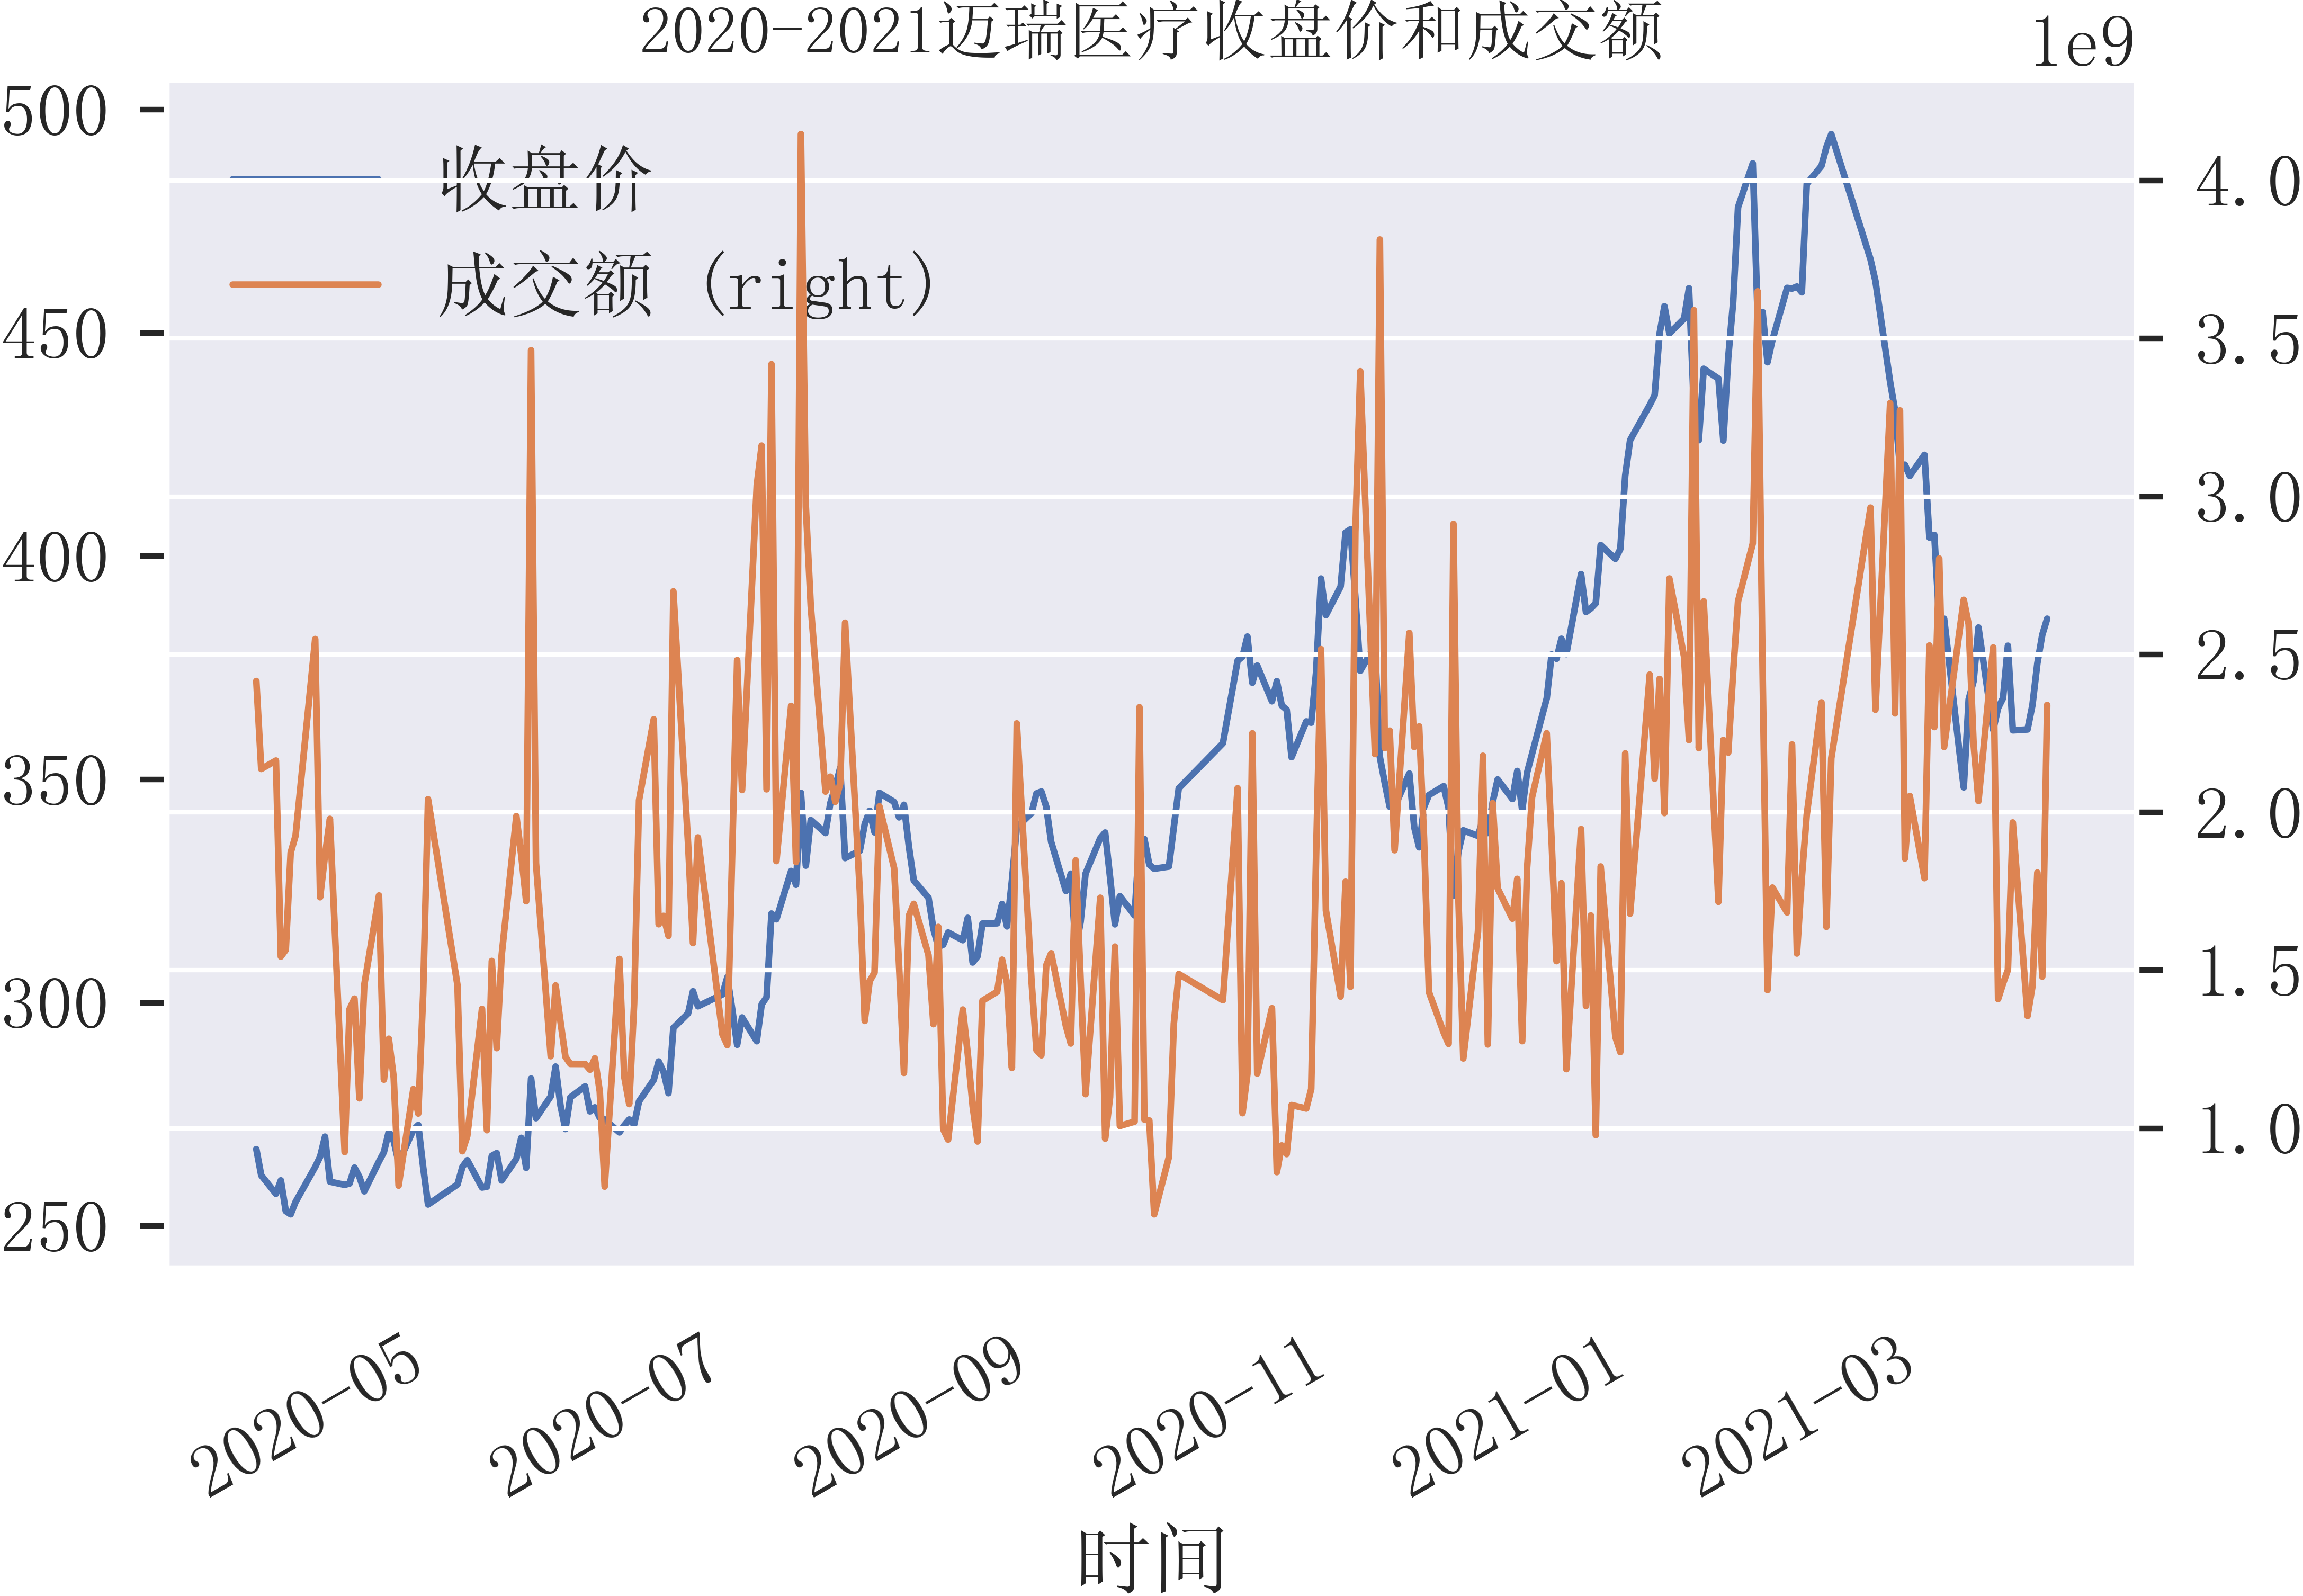
\includegraphics[width=0.8\textwidth]{一年内迈瑞医疗收盘价成交额变化}
		\caption{一年内迈瑞医疗收盘价及成交额变化}
		\label{一年内迈瑞医疗收盘价成交额变化}
	\end{figure}
	\subsubsection{k线图及均线}
	 \begin{figure}[H]
		\centering
		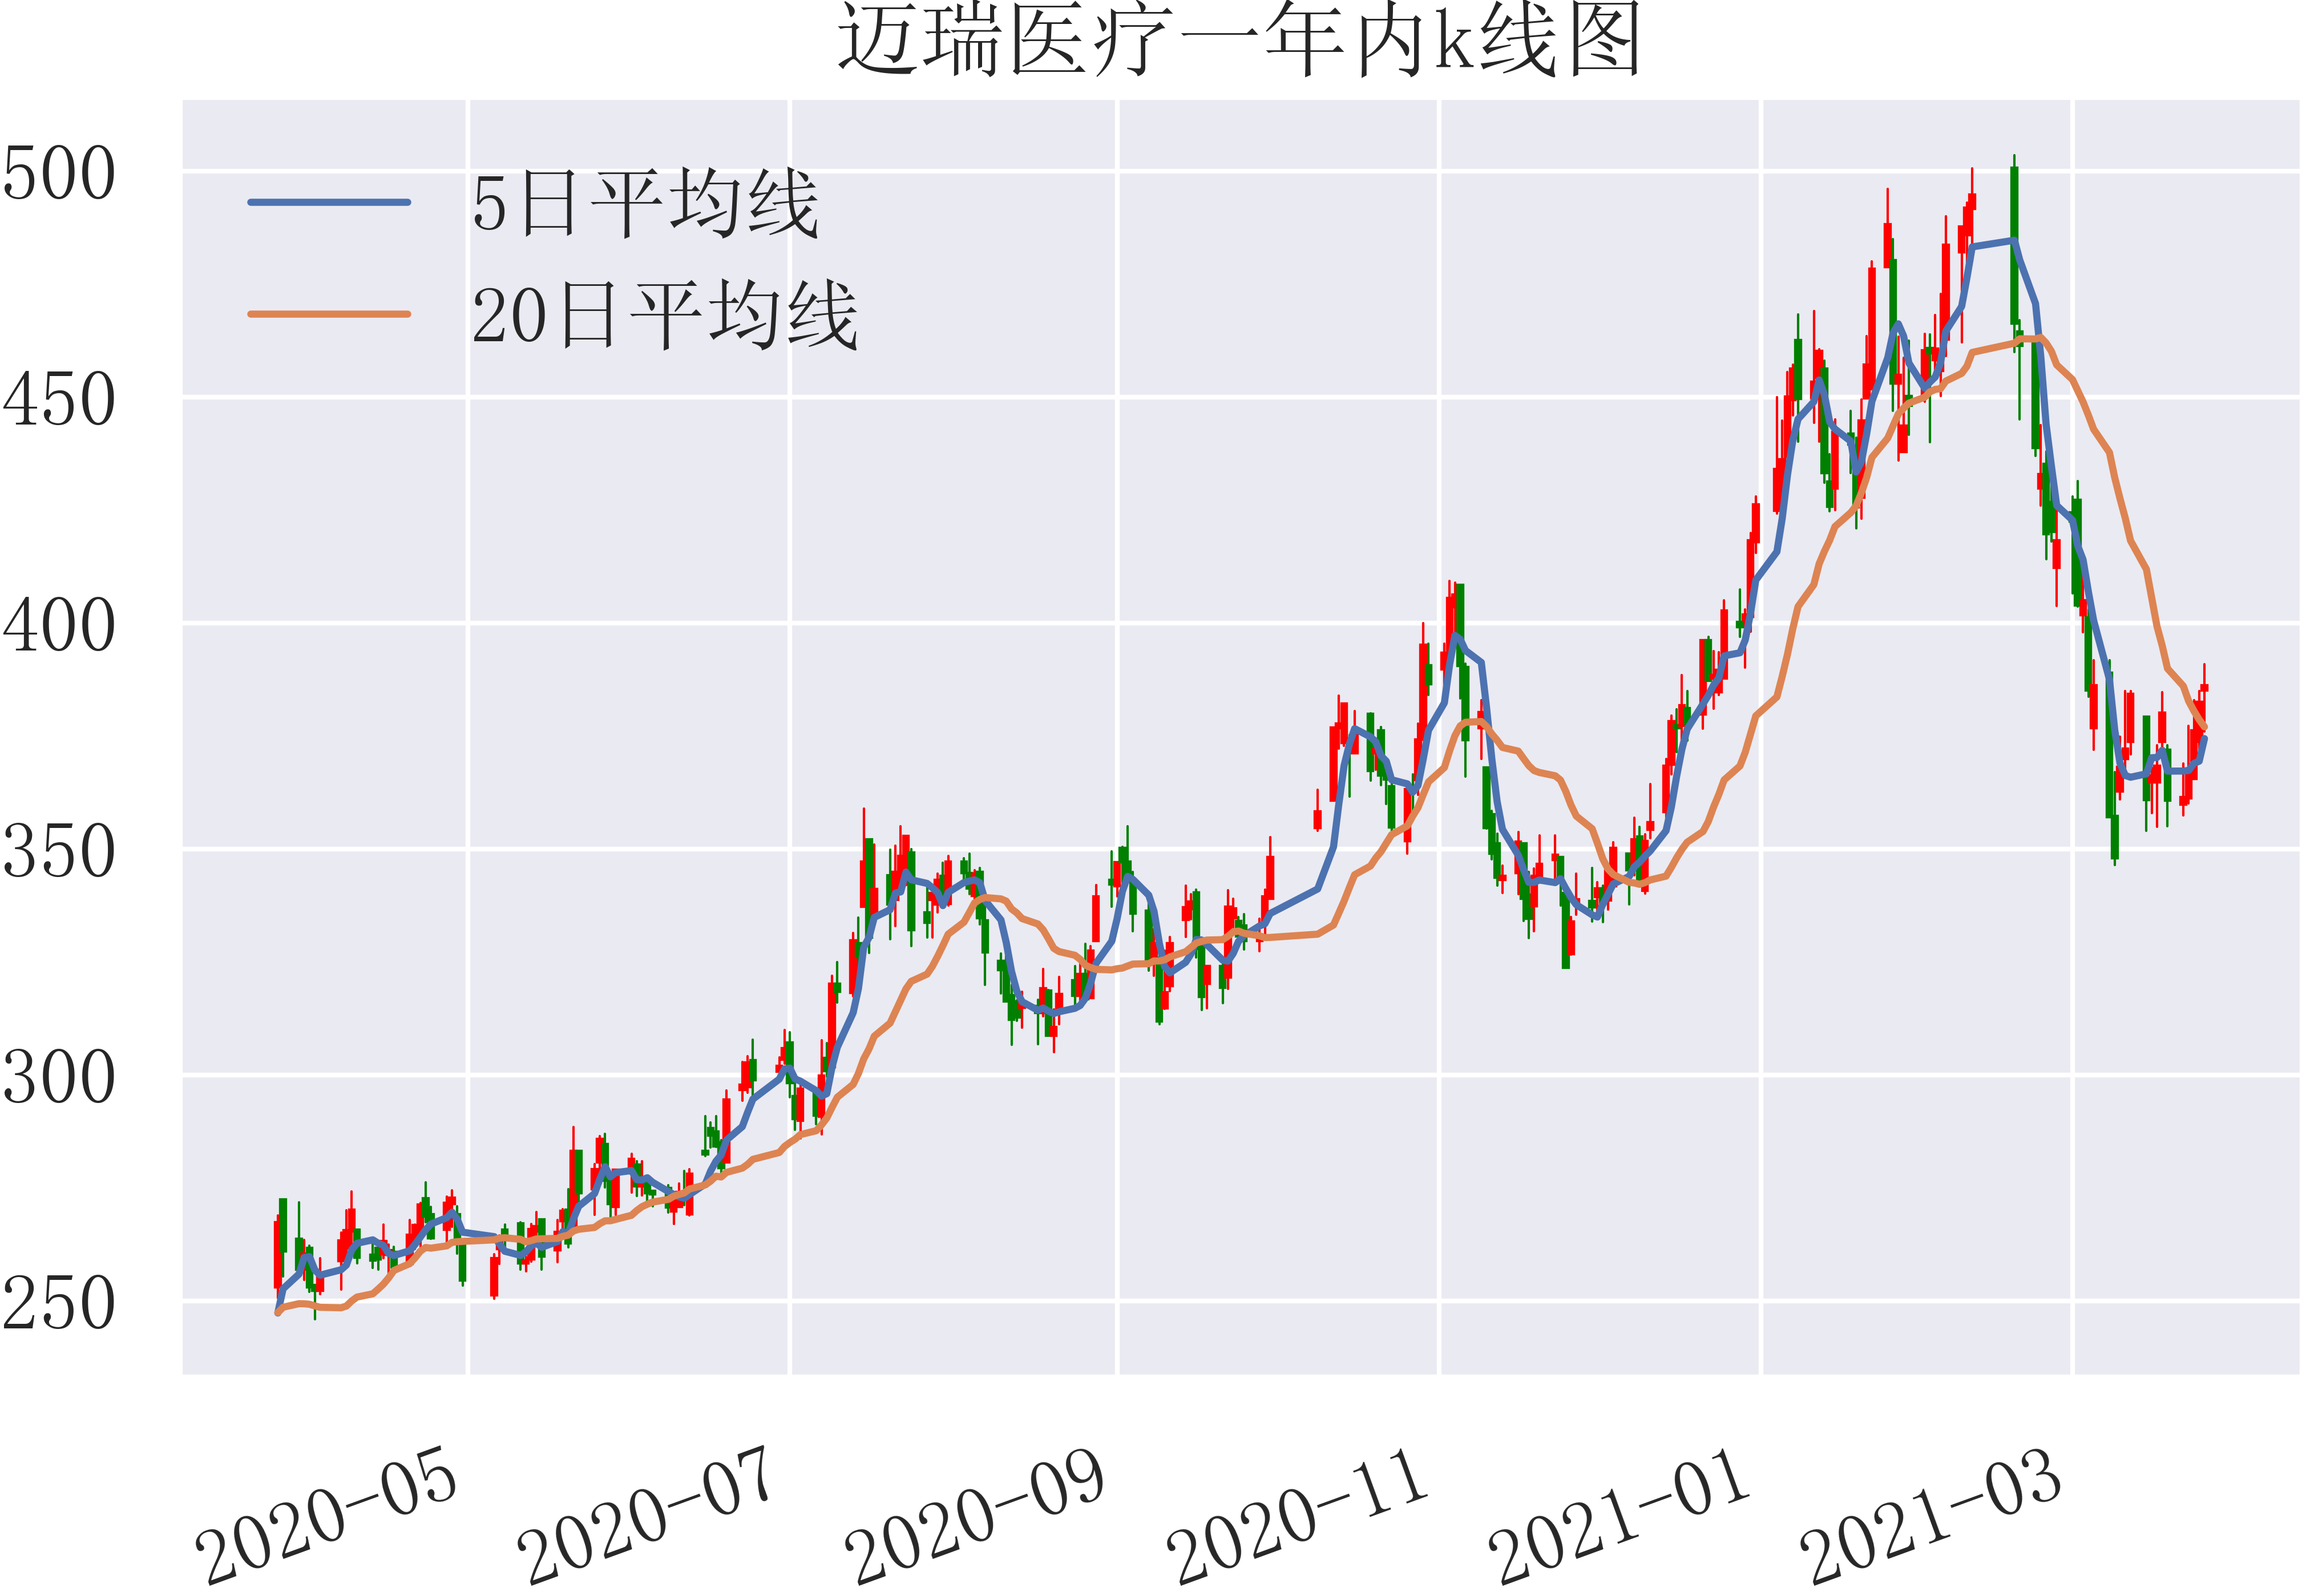
\includegraphics[width=0.8\textwidth]{迈瑞医疗一年内k线图}
		\caption{迈瑞医疗一年内k线图及5日、20日均线}
		\label{迈瑞医疗一年内k线图}
	\end{figure}
	\subsubsection{对数收益率}
	计算收益率的方法有两种:简单收益率和对数收益率(几何收益率)。因为对数收
	益率有优于简单收益率的一些性质:可以实现价格上涨和下降的对称性;使数据变得更
	为平滑;方便计算区间收益率、复利等,因而对数收益率在实际的应用中更为广泛。本
	文用每日收盘价来计算对数收益率,第t 期的对数收益率的计算公式为:
	$$
	r_{t}=\ln p_{t}-\ln p_{t-1}
	$$
	其中$r_t$ 表示某项资产的日收益率,$p_t$ 表示第t 期的资产收盘价。
	迈瑞医疗和片仔癀的收益率的波动图如图所示:
 \begin{figure}[H]
	\centering
	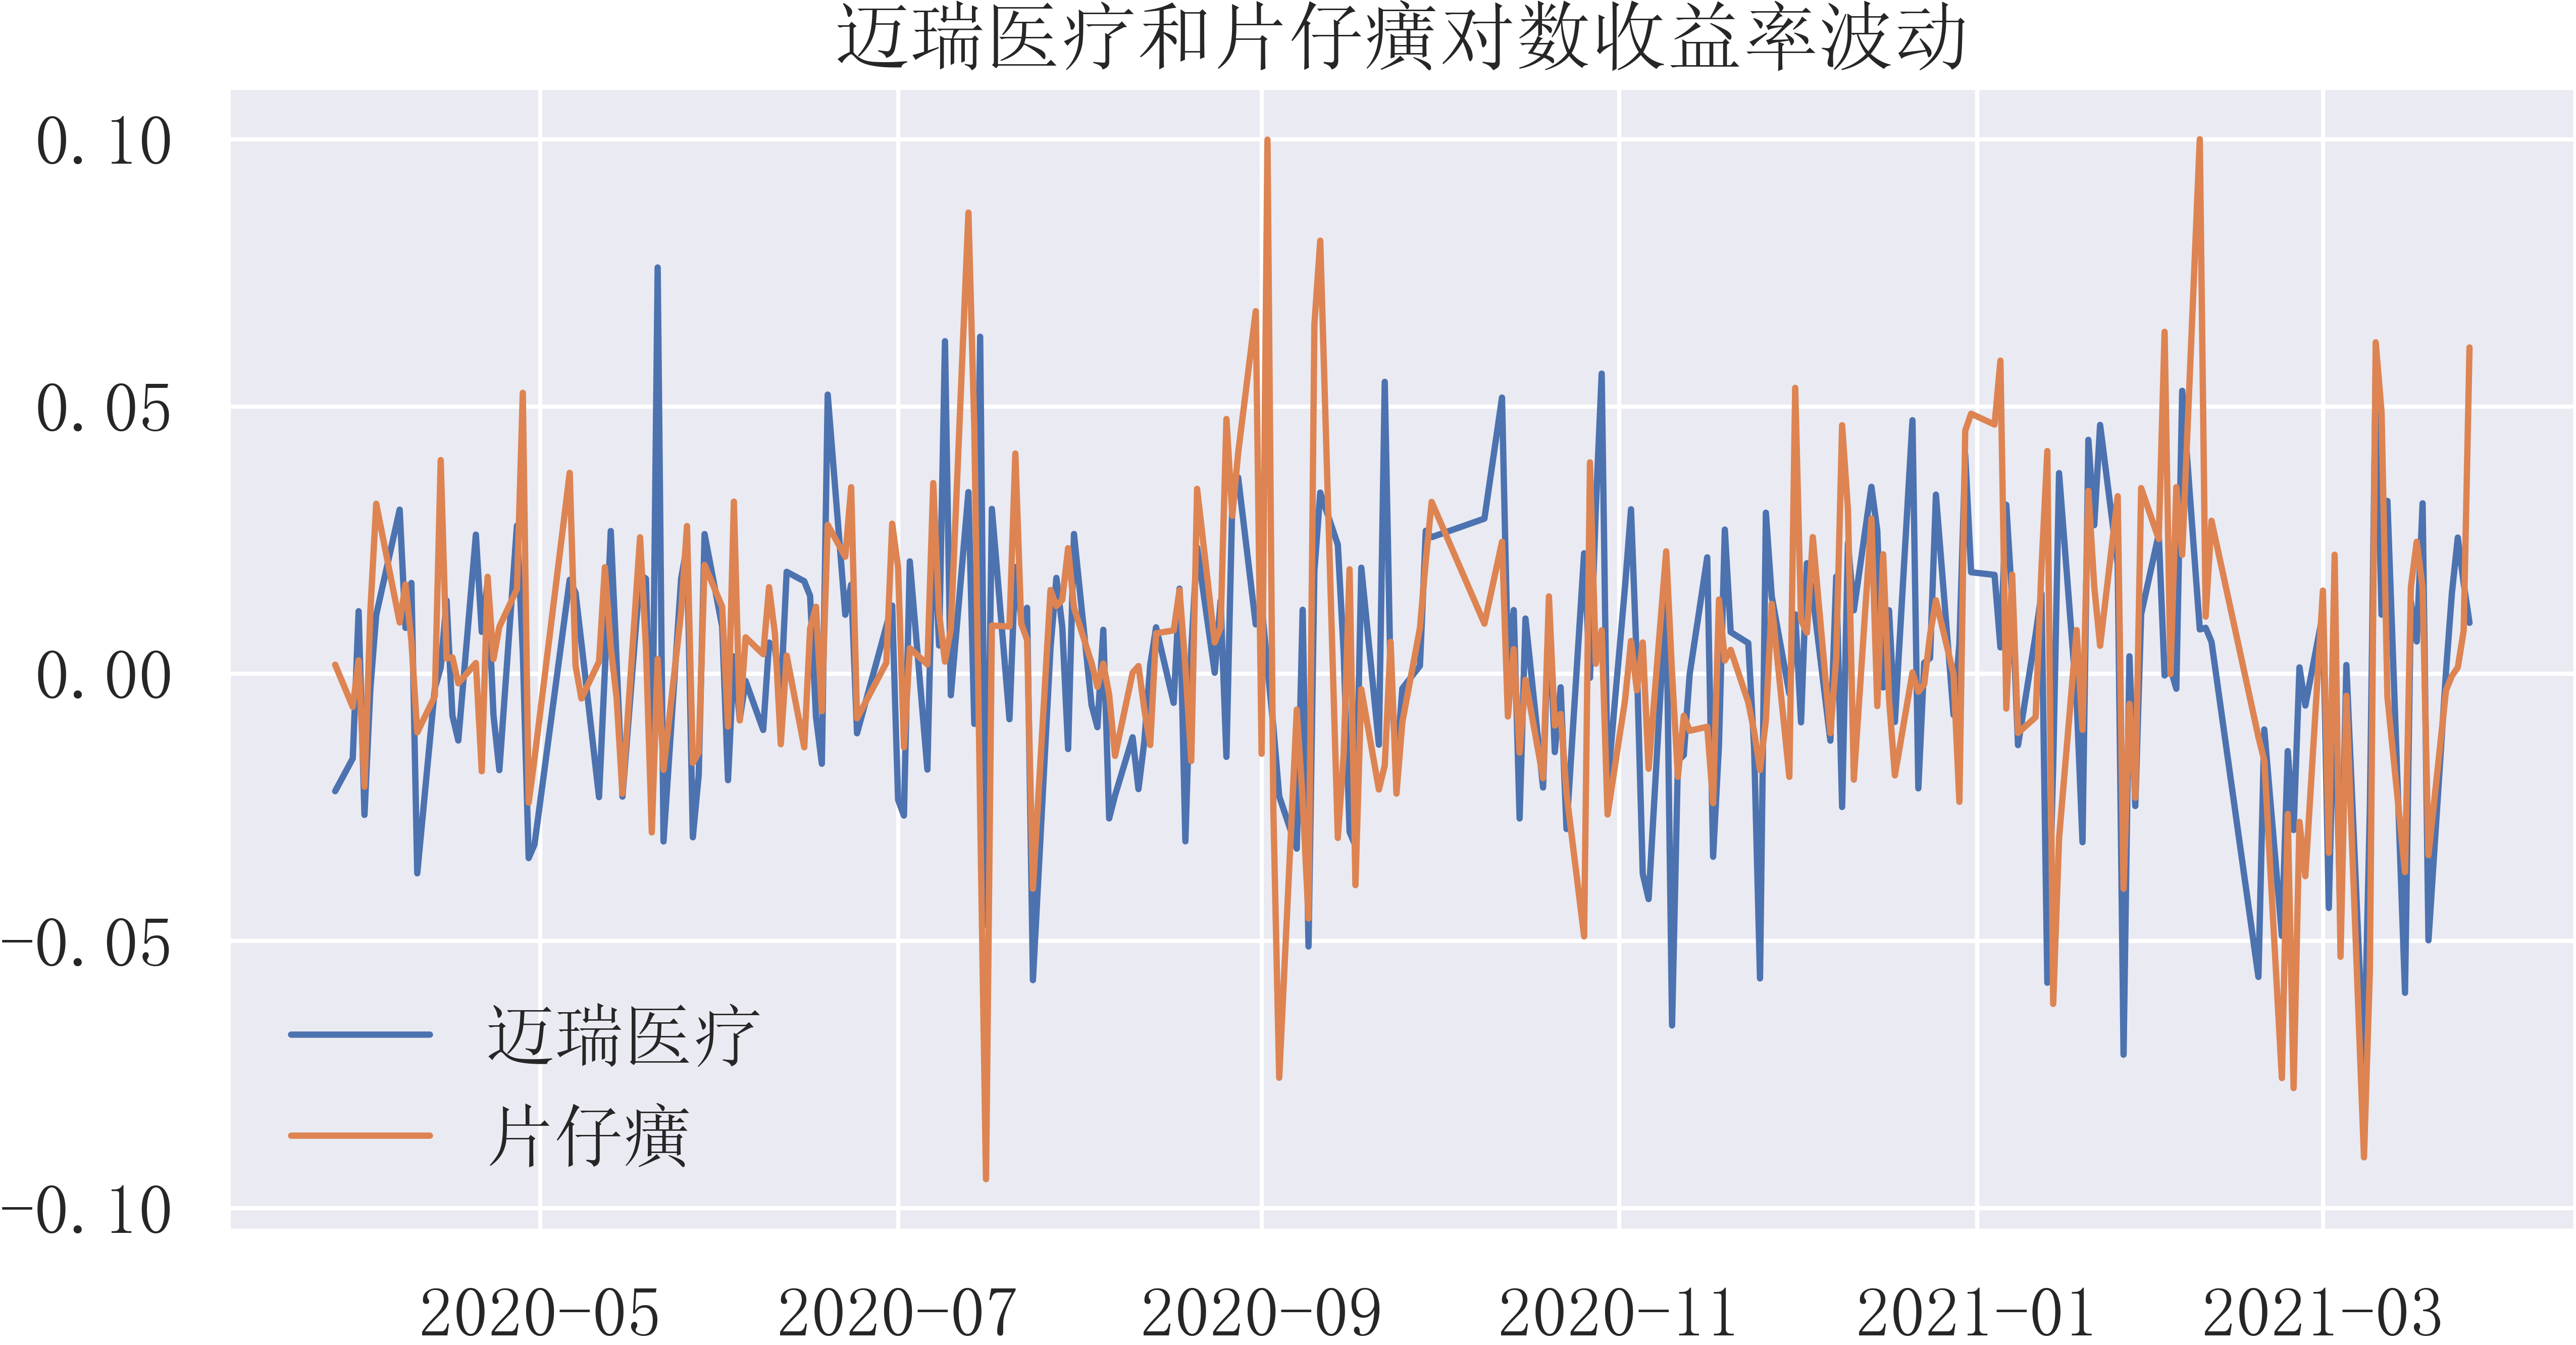
\includegraphics[width=0.8\textwidth]{迈瑞医疗片仔癀对数收益率波动}
	\caption{迈瑞医疗和片仔癀对数收益率波动}
	\label{迈瑞医疗片仔癀对数收益率波动}
\end{figure}
观察上述股票的基本形态,以迈瑞医疗的对数收益率为例,序列的波动在大部分的时段是平稳的,并且围绕着0 值附近波动,大部分时期的波动范围位于-0.05 和0.05 之间。在某些时期波动会持续性地进行,且表现出集聚性的现象。在此期间,其他股票收益率波动图也具有类似特征,
说明了各股票之间也存在一定的相关性。
\subsubsection{相关系数矩阵}
	为了便于观察,对相关系数矩阵进行可视化。
\begin{figure}[H]
	\centering
	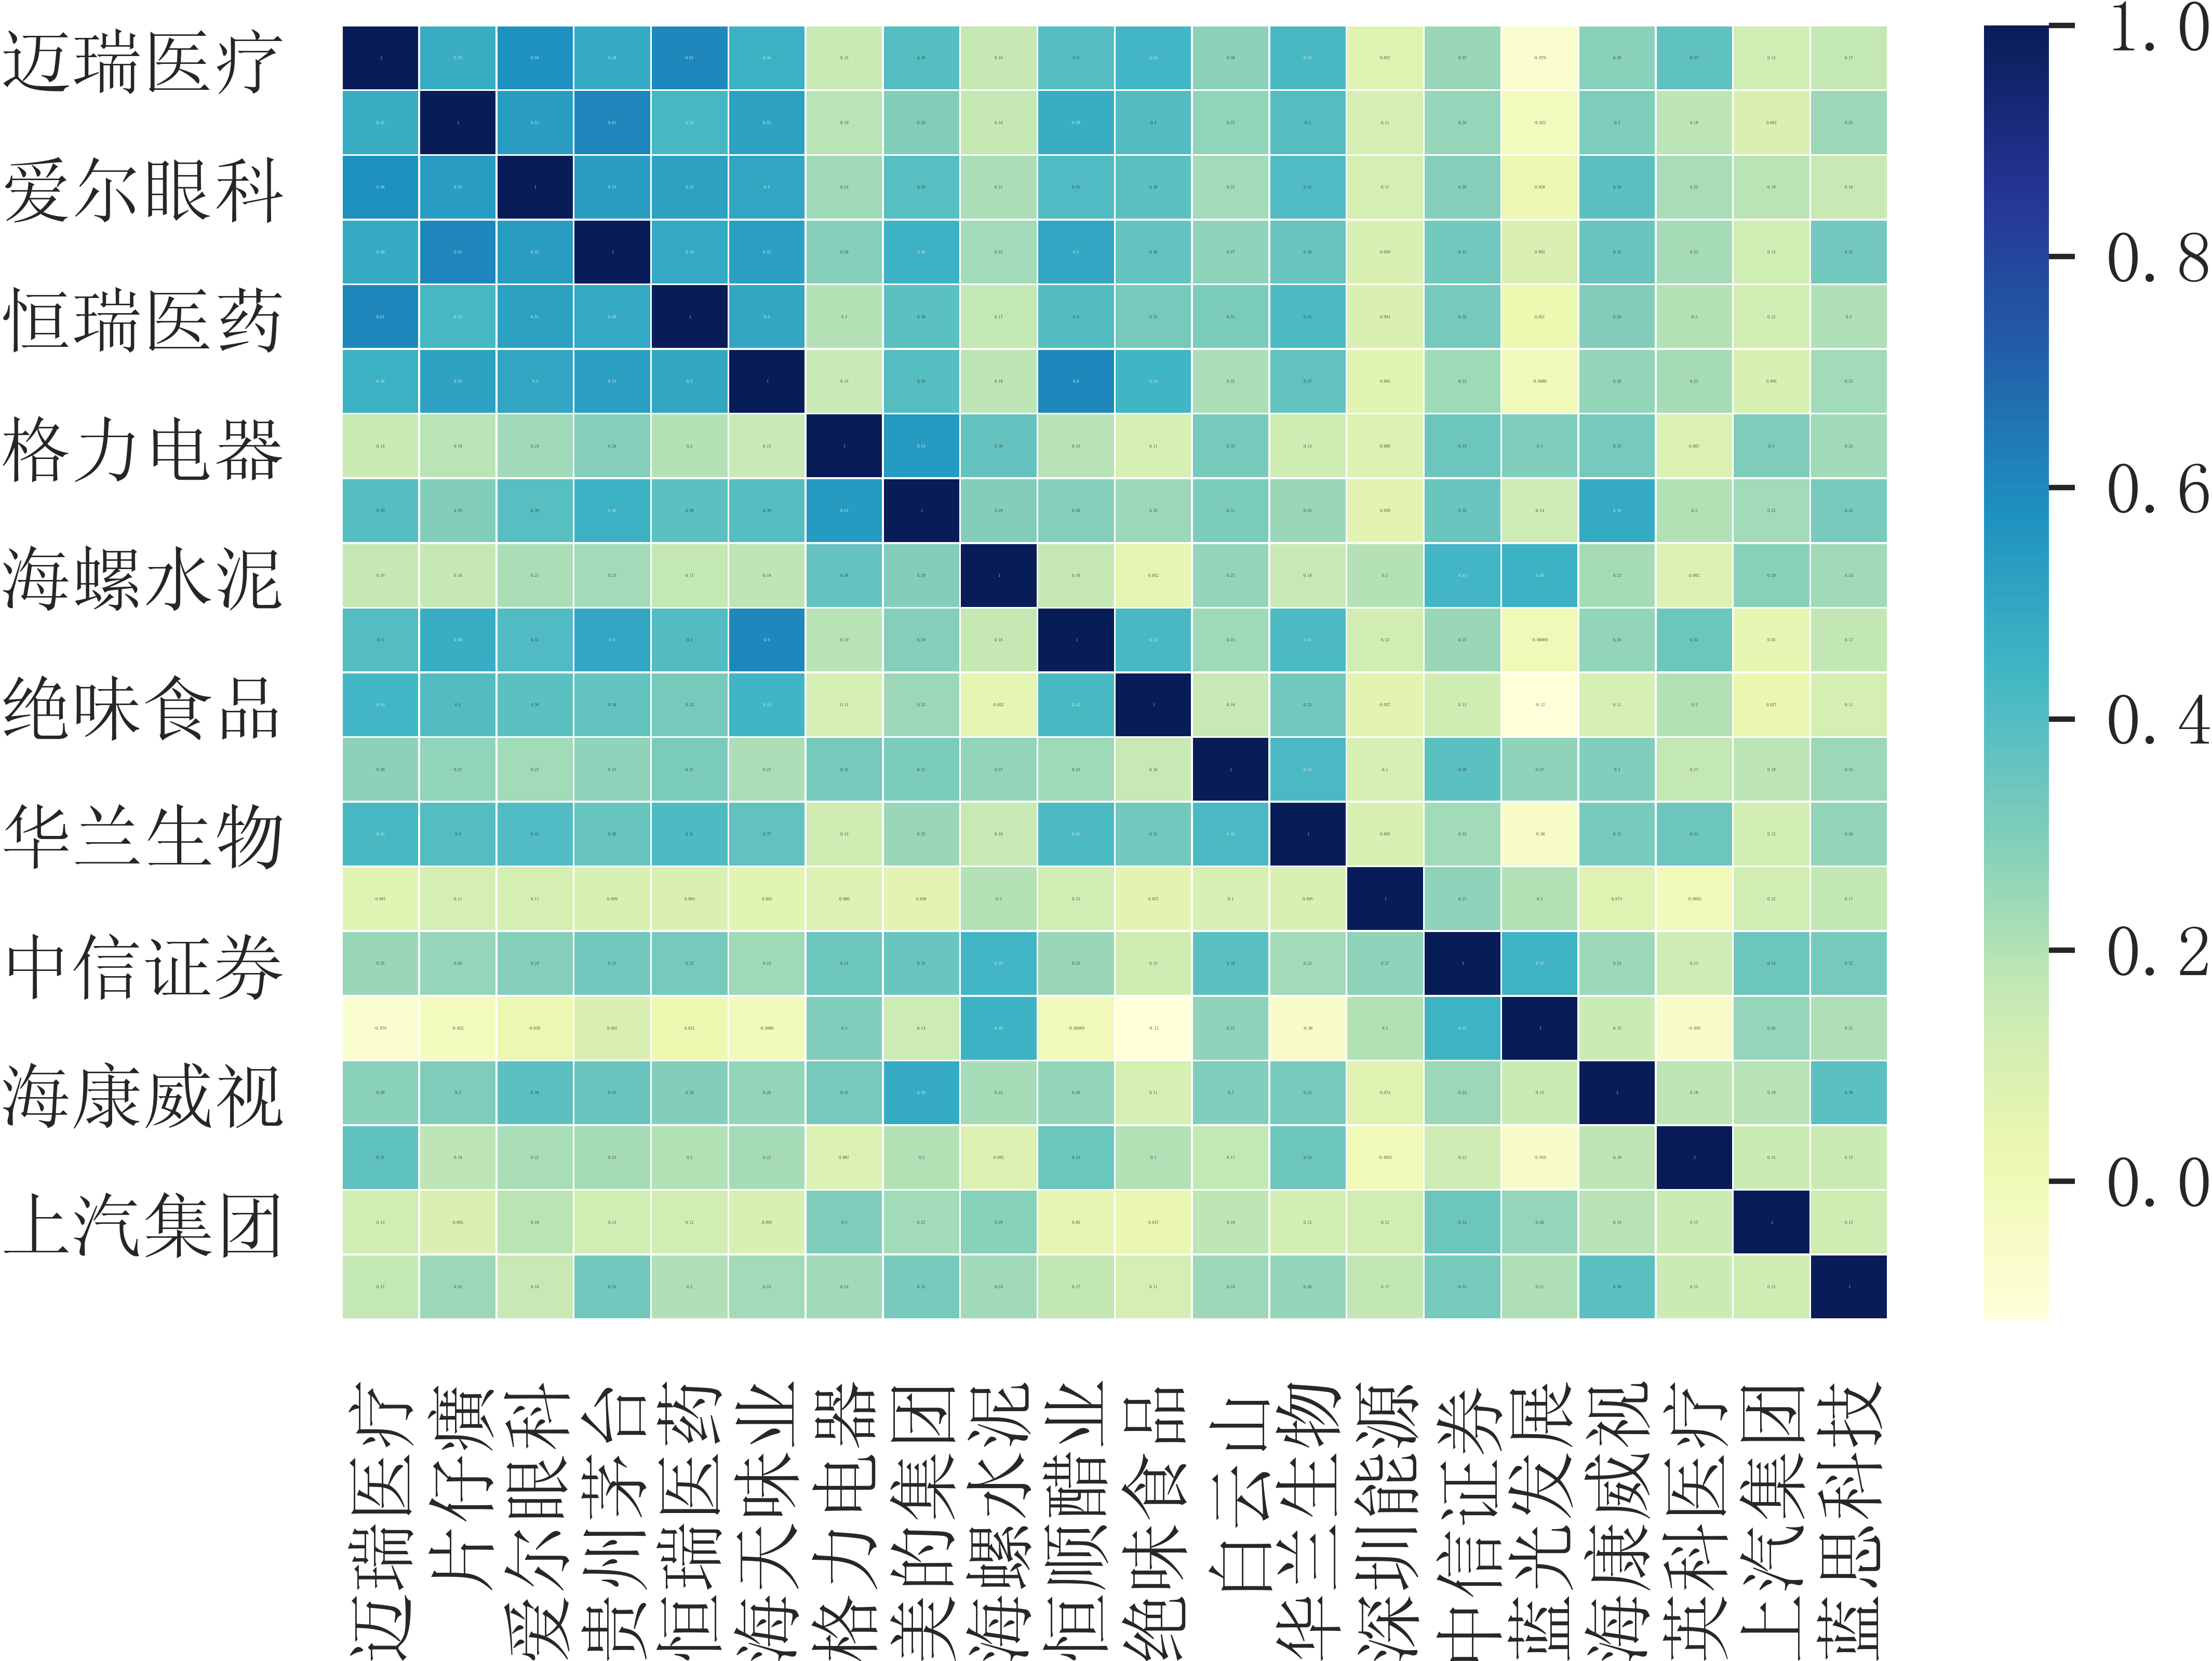
\includegraphics[width=0.7\textwidth]{20种股票相关矩阵}
	\caption{20种股票的相关系数矩阵}
	\label{相关系数矩阵}
\end{figure}
由相关系数矩阵可以明显地看出,迈瑞医疗、片仔癀、爱尔眼科、恒瑞医药等股票具有较大的相关性,原因在于它们都是医疗医药相关行业。

	\subsection{模型的背景}
	针对投资组合方案的选取 本文根据附件20只股票数据来选取最佳的投资方
案。对于投资组合方案的确定,本文可以通过建立组合优化模型来获取最佳的投资方案。
一般来说, 风险资产 的投资首先需要解决的是两个核心问题:即预期收益与风 险。如何
测定组合投资的风险与收益和如何平衡这两项指标进行资产分配也是投资者迫切需要
解决的问题。

投资组合理论研究的是在理性市场中,假定投资者以资产收益的均值表示投
资收益,以资产收益的方差或CVAR表示投资风险,在市场信息完全透明的情况下,投资
者在众多资产组合中寻求帕累托最优解.在投资组合理论的假定框架下,所有可
能最优的均值-风险组合构成平面内的一条曲线,这条曲线被称为有效前沿。
	\subsection{均值-方差模型}
根据马科维茨资产组合理论\upcite{wangJiLeiTouZiZuHeYouHuaMoXingJiQiSuanFa2012},根据投资组合概念,在一定的风险水平上,投资者期
望收益最大;相对应的是在一定的收益水平上,投资者希望风险最小。根据马科维茨
对于投资组合的概念,得知该模型也在追求投资组合风险最小化,符合本文对于最优投
资目标的实现。通过查找资料可以发现投资效用由两个因素所决定,投资者在投资股票
时会考虑到风险以及收益的因素,所有的投资者都会希望收益越大越好,但是收益越大
时,所面临的风险也会越大,会面临亏损的风险。因此投资者也希望风险越小越好。


	Markowitz 基于MV模型构建的投资组合理论系统阐述了投资者如何在期初从
所有可能的资产组合中选取一个最优组合,从而在给定期末收益率水平下使得投
资组合风险最小,或是在给定风险水平下使得期末收益率最大.

假设投资者选择$N $种风险证券进行投资,令$\mu_i$表示第i 个证券的收益率均值,
$\sigma_{i j}$ 表示第$i$ 个证券和第$j $个证券收益率的协方差,决策变量$x_{i}$表示投资在第$i$ 个证
券上的资本比例.则该资产投资组合的收益率$r$ 为各个资产收益率的均值,即:
$$
r=\sum_{i=1}^{N} \mu_{i} x_{i}
$$
各个资产间的方差-协方差矩阵为$\Sigma=\left(\sigma_{i j}\right)_{N \times N}$那么,资产投资组合的风险$\sigma^{2}$为:
\begin{equation}
\sigma^{2}=\sum_{i=1}^{N} \sum_{j=1}^{N} x_{i} x_{j} \sigma_{i j}
\end{equation}
这样,当投资者给定期望收益R 时,为了把投资风险降低到尽可能最小,建立的均值-方差(Mean-Variance,MV)投资组合的最小方差模型可描述为如下形式:
\begin{equation}
\begin{array}{ll}
\min &\sigma^{2}= \sum_{i=1}^{N} \sum_{j=1}^{N} x_{i} x_{j} \sigma_{i j} \\
\text {s.t } & \sum_{i=1}^{N} x_{i} \mu_{i}=R, \\
& \sum_{i=1}^{N} x_{i}=1, \\
& 0 \leq x_{i} \leq 1, \\
& i=1, \ldots, N .
\end{array}
\label{minfc}
\end{equation}	
在给定风险水平下使得期末收益率最大,可建立投资收益最大化模型:
\begin{equation}
\begin{aligned}
&\max r=\sum_{i}^{N} \sum_{j=1}^{N} x_{i} u_{j} \\
&\text {  }\left\{\begin{array}{l}
\sum_{i=1}^{N} \sum_{j=1}^{N} x_{i} x_{j} \sigma_{i j} \leq \sigma_{0}^{2} \\
w_{i} \geq 0 \\
\sum_{i=1}^{n} w_{i}=1
\end{array}\right.
\end{aligned}
\label{maxsy}
\end{equation}
或者综合考虑收益和风险,写成多目标规划形式:
\begin{equation}
\begin{aligned}
&\max r=\sum_{i}^{N} \sum_{j=1}^{N} x_{i} u_{j} \\
&\min \sigma^{2}=\sum_{i=1}^{N} \sum_{j=1}^{N} x_{i} x_{j} \sigma_{i j} \\
&\text { s.t. }\left\{\begin{array}{l}
\sum_{i=1}^{n} x_{i}=1 \\
x_{i} \geq 0, i=1,2, \cdots, N
\end{array}\right.
\end{aligned}
\label{dmb}
\end{equation}
引入风险规避参数$\lambda \in[0,1]$后,问题(\ref{dmb})等价于问题(\ref{lamda})
\begin{equation}
\begin{array}{ll}
\min & \lambda\left[\sum_{i=1}^{N} \sum_{j=1}^{N} x_{i} x_{j} \sigma_{i j}\right]-(1-\lambda)\left[\sum_{i=1}^{N} x_{i} \mu_{i}\right] \\
\text { s.t. } & \sum_{i=1}^{N} x_{i}=1 \\
& 0 \leq x_{i} \leq 1 \\
& i=1, \ldots, N
\end{array}
\label{lamda}
\end{equation}
当$\lambda =0$时,表示仅最大化投资组合期望收益率,这时最优解由最大收益率的
资产组成,即最大收益模型(\ref{maxsy}).当$\lambda =1$时,表示仅选取投资组合风险最小的组合进行投资,即最小方差模型(\ref{minfc}).对于每个
$\lambda \in[0,1]$,求解问题,都会得到一对期望收益率和风险值,所有这些值就组成
了问题的有效前沿.

定义夏普比率(SharpeRatio)
\begin{equation}
\text { SharpeRatio }=\frac{E\left(R_{p}\right)-R_{f}}{\sigma_{p}}
\end{equation}
其中,$E(R_{p})$ 表示投资组合预期收益,$R_f$
表示无风险资产收益,$\sigma_p$表示投资组合的风险。

夏普比率指的是每单位风险资产的超额收益,可以很好地衡量投资组合中投资者每承受一单位风
险会产生多少超额回报。以夏普比率为目标函数,式(\ref{dmb})可以改写为:
\begin{equation}
\begin{array}{ll}
\max &\text { SharpeRatio }=\frac{\sum_{i=1}^{N} x_{i} \mu_{i} -R_f }{\sqrt{\sum_{i=1}^{N}\sum_{j=1}^{N} x_{i} x_{j} \sigma_{i j}}}  \\
\text { s.t. } & \sum_{i=1}^{N} x_{i}=1 \\
& 0 \leq x_{i} \leq 1 \\
& i=1, \ldots, N
\end{array}
\end{equation}
求解以夏普比率为目标函数的方程,可以得到夏普比率时的投资组合,即从有效前沿中选择夏普比率最大的投资组合。

Markowitz 均值-方差模型及其相关变体是投资决策中最基础的投资模型,是投资组合理论最核心的数量化模型。其余的优化模型都是在均值-方差模型的基础上的扩展模型,只是它们对风险的描述方法有所不同,但描述资产组合收益率的变量却是相同的。
	\subsection{均值-CVAR模型}
	Markowitz 提出的投资组合理论是进行投资组合研究的一个起点,其模型建立
	在理想化假设下,很难精确反映资本市场的实际情况.鉴于这一原因,此后很多
	学者基于该模型进行了一系列模型改进和理论完善的研究工作.
	\subsubsection{VaR和CVaR风险度量方法}
	VaR 方法是从风险管理的实践中产生的新型风险管理方法\upcite{wangJiYuCVaRFengXianCeDuDeHouHuiZuiXiaoHuaTouZiZuHeMoXing2021}。VaR 方法的出现,
	给风险管理领域带来了革命性的变革,并迅速成为广受欢迎的风险度量工具。
	
	VaR(Value at Risk),译为在险价值\upcite{wangJiYuCVaRFengXianCeDuDeHouHuiZuiXiaoHuaTouZiZuHeMoXing2021,wangKaoLuJiaoYiFeiYongDeJunZhiVaRDuoJieDuanTouZiZuHeYouHuaMoXing2020},是在一定的置信水平下,投资工具在一定
	持有期内的最坏的预期损失。如果$X$ 表示随机损失,$X$ 的分布函数为$F_{X}(x)$ ,VaR
	就是在给定的概率水平$\alpha \in(0,1)$下的最大可能损失
$$
P_{r}\left\{X \leq \operatorname{VaR}_{\alpha}(X)\right\}=\alpha
$$
	即 $\operatorname{VaR}_{\alpha}(X)=F_{X}^{-1}(\alpha)$
	
	或者$\operatorname{VaR}_{a}(X)=\min \left\{x \mid F_{X}(x) \geq \alpha\right\}$.
	
	VaR的含义说明损失$X$ 超过$\operatorname{VaR}_{\alpha}(X)$的概率不大于$1-\alpha$,是一个小概率事件。
	$\alpha$ 的取值与投资者的风险偏好水平相关,通常取值为95\%或99\%。不难看出,VaR
	就是随机变量$X$ 的$\alpha$ 分位数。换种角度来说,VaR 方法从概率的角度解决了最大
	损失的度量问题。
	
	由 VaR 的定义可以知道,VaR 是在给定置信水平和持有期的条件下,投资工
	具或组合潜在损失的最大值。VaR 本质上是是随机变量$X$ 的$\alpha$ 分
	位数,由此导致了在VaR 的计算是不充分的,在计算过程中忽略了损益分布的厚
	尾信息。尽管如此,VaR 方法仍然是现代金融风险度量理论的标准方法,在风险管理
	中得到广泛的使用,也适用于投资者对风险的把控。
	
	为了弥补 VaR 的缺陷,条件风险价值(CVaR)的概念在二十一世纪初被提出\upcite{zhangJiBenZhiShuZuiXiaoXiaBanFangChaiTouZiZuHeYouHuaYanJiu2021},
	它是在VaR 方法的基础上发展起来的,是对VaR 方法的拓展,比VaR 方法更加全
	面。
	
	CVaR 是指在在一定的置信水平下,一定的持有期内投资工具的损失超过VaR
	极端的期望值。简单地讲,CVaR 就是投资损失超过VaR 值的条件均值,代表了超
	额损失的平均水平。其公式为:
	\begin{equation}
	C V a R_{\alpha \alpha}(\gamma)=E\left(\gamma \mid \gamma \geq \operatorname{VaR}_{\alpha}(\gamma)\right)=\frac{1}{1-\alpha} \int_{f(x, y) \geq \mu_{\alpha}(x)} f(x, y) p(y) d y
	\end{equation}
	其中$\gamma$ 表示组合损失;$f (x, y)$是一个随机向量,为投资组合的损益函数;$X $为
	投资组合的可行集;$x$ 是投资组合各资产的权重向量,且
	$x \in X \subset R^{n}$;$y$ 是市场的
	价格向量。
	在实证分析中, $x$ 可理解为用于配置各种资产的资金比例, $X$ 为所有可行的
	投资组合的集合,$y$ 为引起投资组合发生亏损的市场因子。需要说明的是,损失为
	负值等同于有正的收益。
	
	对任意给定的$x$, $y$的分布密度函数为$P( y)$,假定y为连续型随机变量,对任意
	$\mu \in R$,令
$\Psi(x, \mu)=\int_{f(x, y) \leq \mu} p(y) d y$
$\Psi(x, \mu)$为累积概率分布函数,关于$\mu$是递增的,对任意$\mu \in(0,1)$,定义:
\begin{equation}
\begin{gathered}
\mu_{\alpha}(x)=\min \{\mu \in R: \Psi(x, \mu) \geq \alpha\} \\
\varphi_{\alpha}(x)=E\left[f(x, y) \mid f(x, y) \geq \mu_{\alpha}(x)\right]=\frac{1}{1-\alpha} \int_{f(x, y) \geq \mu_{\alpha}(x)} \int f(x, y) p(y) d y
\end{gathered}
\end{equation}
	则$\mu_{\alpha}(x)$ 和$\varphi_{\alpha}(x)$就是置信水平为$\alpha$的VaR 和CVaR。
	
	CVaR 是一个凸函数,能够利用一个最小化的公式表示出来,并可转换为线性
	规划进行求解,更易于求出,这是CVaR 优于VaR 的重要原因之一。
	CVaR 是损失超过VaR 的条件均值,是满足一致性公理的风险度量工具,较之
	VaR 更为全面,更能体现出潜在风险;
	
当可行集$X \subset R^{n}$时,求解 CVaR 的值就可以转化
	为求以下函数的最小值,令
$$
F_{\alpha}(x, \theta)=\theta+\frac{1}{1-\alpha} \int_{y \in R^{m}}[f(x, y)-\theta]^{+} p(y) d y
$$
其中,$$
[f(x, y)-\theta]^{+}=\max [f(x, y)-\theta, 0]
$$
则有:
$$
\phi(x)=\min _{\theta} F_{\alpha}(x, \theta)
$$
	通过对函数$F_{\alpha}(x, \theta)$进行最小化,可以同时求出 VaR 和优化的 CVaR。求解最小CVaR 的问题就转换为一个凸函数的求极值问题\upcite{zhangQiuJieTouZiZuHeYouHuaWenTiDeHunHeErCiGuiHuaHeQiFaShiSuanFa2019,zhouJiYuFengXianDuLiangCVaRDeGuPiaoShiChangTouZiZuHeYouHua2020a},求出的极小值就是CVaR,相
	应的极小值点便是VaR。
	\subsubsection{均值-CVaR模型的建立}
	根据 Markowitz 均值-方差模型以及CVaR 方法的介绍,可以建立均值-CVaR
	模型为
	\begin{equation}
	\begin{aligned}
	&\min C V a R_{\alpha}\left(x^{T} R\right)\\
	&\text { s.t. }\left\{\begin{array}{l}
	E\left(x^{T} R\right) \geq r_{0} \\
	x^{T} I=1 \\
	x \geq 0
	\end{array}\right.
	\end{aligned}
	\end{equation}
	或者:
	\begin{equation}
	\begin{aligned}
	&\max _{x} E\left(x^{T} R\right) \\
	&\text { s.t }\left\{\begin{array}{l}
	\text { CVaR }_{\alpha}\left(x^{T} R\right) \leq W_{0} \\
	x^{T} I=1 \\
	x \geq 0
	\end{array}\right.
	\end{aligned}
	\end{equation}
	
其中$R=\left(r_{1}, r_{2}, \ldots, r_{n}\right)^{T}$, $r_i$ 为第$i$ 种资产的收益率, $r_0$为投资者的投资组合的期
望回报率,$W_0$ 为投资者可承受的风险水平上限,$I=(1,1, \cdots, 1)^{T}$。
由 CVaR 定义给出的数学表达式可知,资产的损益函数可以表示为:
$$
f(x, R)=-x^{T} R
$$
那么,
$$
\hat{F}_{\alpha}(x, \theta)=\theta+\frac{1}{1-\alpha} \int_{R \in R^{n}}\left[-x^{T} R-\theta\right]^{+} p(y) d y
$$
当使用离散样本来估计上述模型中组合中各资产的权重$x $与CVaR 时,
$R_{1}, R_{2}, \ldots, R_{J}$为来自总体R 的样本,有
$$\hat{F}_{a}(x, \theta)=\theta+\frac{1}{J(1-\alpha)} \sum_{k=1}^{J}\left[-x^{T} R^{k}-\theta\right]^{+}$$
\begin{equation}\label{111}
\hat{F}_{\alpha}(x, \theta)=\theta+\frac{1}{J(1-\alpha)} \sum_{k=1}^{J}\left[-x_{k} r_{k}-\theta\right]^{+}
\end{equation}

令$d_{k}=\left[-x_{k} r_{k}-\theta\right]^{+}$,则式(\ref{111})可以用关于$d_k$ 的线性函数$\theta+\frac{1}{J(1-\alpha)} \sum_{k=1}^{J} d_{k}$和线性约
束$d_{k} \geq-x_{k} r_{k}-\theta, d_{k} \geq 0$来表示。
因此,可以得到基于样本的均值-CVaR 的投资组合优化模型:
\begin{equation}
\begin{aligned}
&\min _{x, \theta} \hat{F}_{a}(x, \theta)=\theta+\frac{1}{J(1-\alpha)} \sum_{k=1}^{J} d_{k} \\
&\text { s.t. }\left\{\begin{array}{l}
\hat{E}\left(R_{p}\right)=x^{T} \bar{R} \geq r_{0} \\
d_{k} \geq-x_{k} r_{k}-\theta \\
d_{k} \geq 0 \\
\sum_{i=1}^{n} x_{i}=1 \\
0 \leq x_{i} \leq 1
\end{array}\right.
\end{aligned}
\end{equation}
或者:
\begin{equation}
\begin{aligned}
&\max _{x, \theta} R_{p}=x^{T} \bar{R} \\
&\text { s.t }\left\{\begin{array}{l}
\theta+\frac{1}{J(1-\alpha)} \sum_{k=1}^{J} d_{k} \leq W_{0} \\
d_{k} \geq-x^{T} R^{k}-\theta \\
d_{k} \geq 0 \\
\sum_{i=1}^{n} x_{i}=1 \\
0 \leq x_{i} \leq 1
\end{array}\right.
\end{aligned}
\label{rp}
\end{equation}
其中, $x^{T} \bar{R}$为资产组合的期望收益率,$\bar{R}=\frac{1}{J} \sum_{k=1}^{J} R^{k}$为资产组合资产的期望收益率向量。
与均值-方差模型类似,式(\ref{rp})表明在既定的收益水平$r_0$ 下使得资产组合的
风险最小化,模型表明在投资者允许的风险水平$W_0$ 下使得资产组合的收益最大化。

同夏普比率的定义一样,定义条件夏普比率(Conditional SharpeRatio)
\begin{equation}
\text { Conditional SharpeRatio }=\frac{E\left(R_{p}\right)-R_{f}}{CVaR}=\frac{E\left(R_{p}\right)-R_{f}}{\hat{F}_{a}(x, \theta)}
\end{equation}
以条件夏普比率为目标函数:
\begin{equation}
\begin{aligned}
&\max \frac{E\left(R_{p}\right)-R_{f}}{\hat{F}_{a}(x, \theta)} \\
&\text { s.t }\left\{\begin{array}{l}
\hat{E}\left(R_{p}\right)=x^{T} \bar{R} \geq r_{0} \\
\theta+\frac{1}{J(1-\alpha)} \sum_{k=1}^{J} d_{k} \leq W_{0} \\
d_{k} \geq-x^{T} R^{k}-\theta \\
d_{k} \geq 0 \\
\sum_{i=1}^{n} x_{i}=1 \\
0 \leq x_{i} \leq 1
\end{array}\right.
\end{aligned}
\end{equation}
条件夏普比率代表收益与风险的均衡,在实际的求解中我们往往选择该模型而不是收益最大化或者风险最小化的模型。
	\subsection{因子分析选取股票}
	\subsubsection{相关性检验}
	因子分析是将多指标化为少数几个综合指标的一种统计分析方法,该方法主
	要是通过降维技术把多个变量化为少数几个主成分,构造出新的主成分方程,通
	过这些主成分来反映原始变量所包含的大部分信息\upcite{an10ZhiZuiYouQianLiDeGuPiao2013}。
	
	数据来源于附件中的数据。选取收盘价、开盘价、最高价、最低价、涨跌幅、涨跌额、成交量、成交额、振幅、换手率11个财务指标进行标准化处理,构造相关系数矩阵:
	
	 \begin{figure}[H]
		\centering
		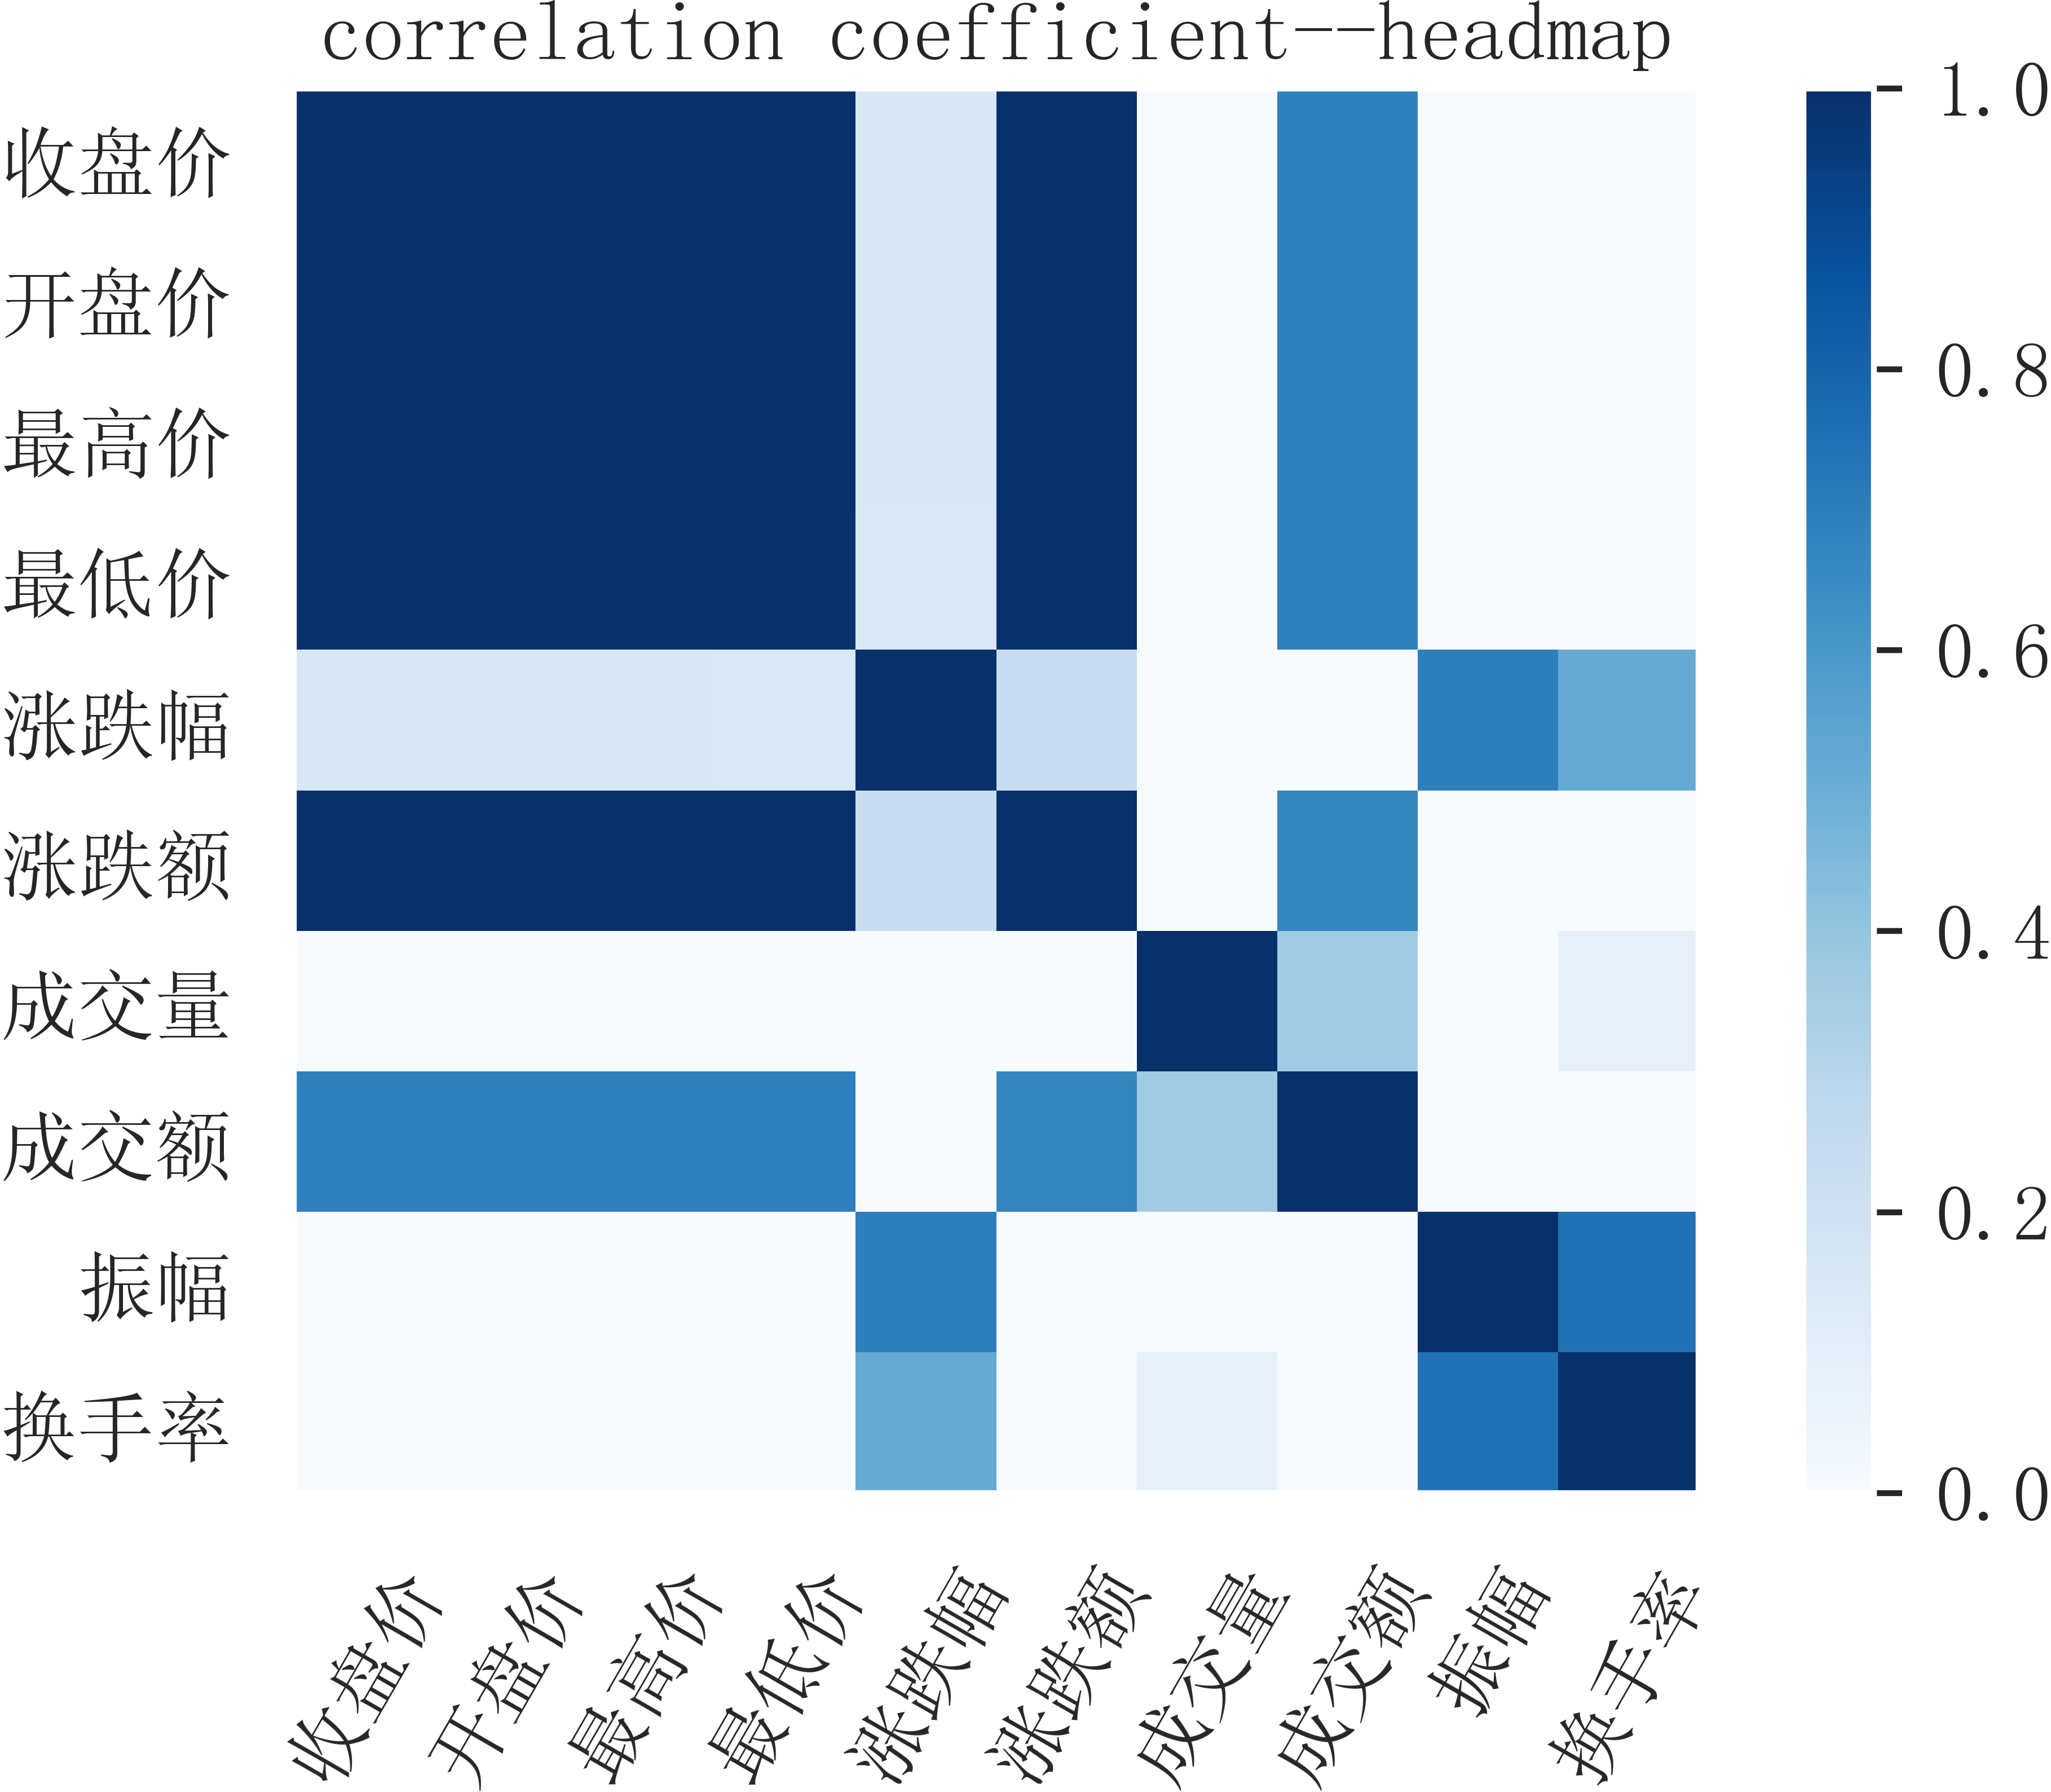
\includegraphics[width=0.6\textwidth]{correlation coefficient--headmap}
		\caption{11个财务指标相关系数矩阵}
		\label{11个财务指标相关系数矩阵}
	\end{figure}
	可以看到,11个财务指标之间的相关系数很高。
	
	\subsubsection{KMO检验和巴特利特球形检验}
	对数据进行KMO检验和巴特利特球形检验\upcite{liuJiYuYinZiFenXiFangFaDeTouZiJieZhiPingGu2020},计算的KMO测度为0.7,大于0.6,巴特利特球形检验的P值为0,因此指标的选择比较合理,适合做因子分析。
	\subsubsection{因子分析}
	对11个财务指标进行因子分析,得到各因子的贡献值如下:
	
		 \begin{figure}[H]
		\centering
		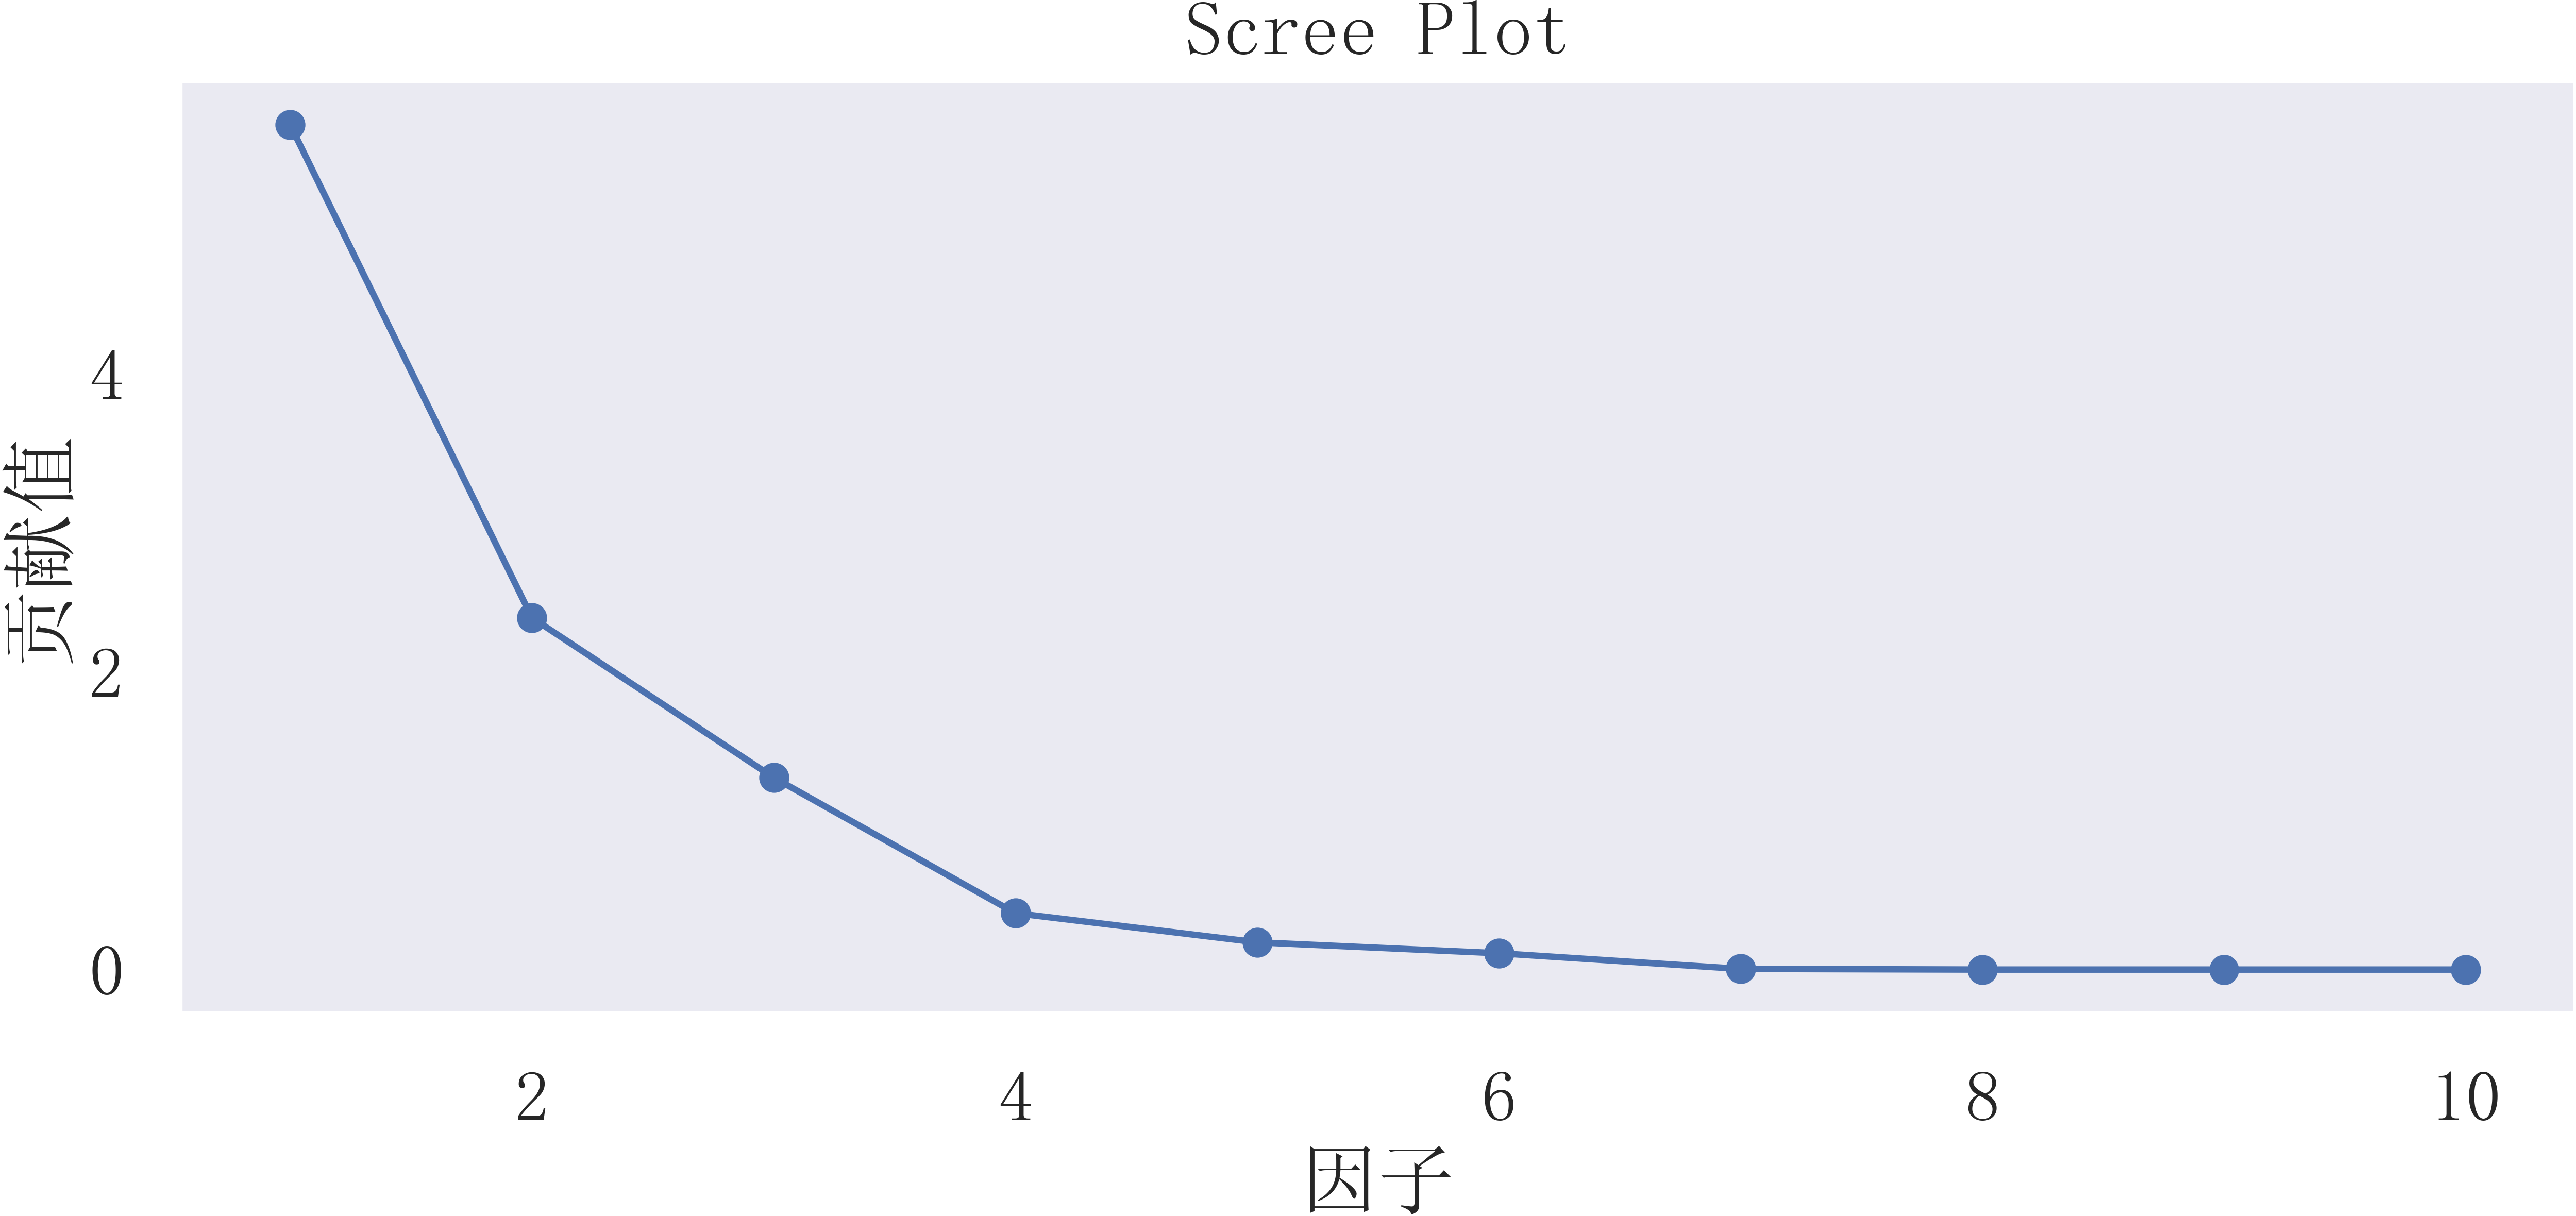
\includegraphics[width=0.8\textwidth]{ScreePlot}
		\caption{各因子的贡献值}
		\label{各因子的贡献值}
	\end{figure}
% Table generated by Excel2LaTeX from sheet 'Sheet1'
\begin{table}[htbp]
	\centering
	\caption{贡献率和累积贡献率}
	\begin{tabularx}{\textwidth}{@{}c *6{>{\centering\arraybackslash}X}@{}}
		\toprule[1.5pt]
		& \multicolumn{1}{c}{\textbf{因子1}} & \multicolumn{1}{c}{\textbf{因子2}} & \multicolumn{1}{c}{\textbf{因子3}} & \multicolumn{1}{c}{\textbf{因子4}} & \multicolumn{1}{c}{\textbf{因子5}} & \multicolumn{1}{c}{\textbf{因子6}} \\
		\midrule
		\textbf{特征值} & 5.67  & 2.32  & 1.23  & 0.33  & 0.13  & 0.08 \\
		\textbf{贡献率} & 0.57  & 0.23  & 0.12  & 0.03  & 0.01  & 0.01 \\
		\textbf{累计贡献率} & 0.57  & 0.80  & 0.92  & 0.95  & 0.97  & 0.98 \\
		\bottomrule[1.5pt]
	\end{tabularx}%
	\label{贡献率和累积贡献率}%
\end{table}%

从图\ref{各因子的贡献值}和表\ref{贡献率和累积贡献率}中可以看出,前3个因子的累积贡献率已经大于90\%,因此选取前3个因子,基本可以反映10 个
指标所反映的信息,这里既减少了指标变量的个数,又便于对问题进行全面分析
和研究。之后计算因子载荷矩阵,为了直观看出公因子与原指标的关系,同样使用热力图对相应的矩阵进行了可视化展示。
		 \begin{figure}[H]
	\centering
	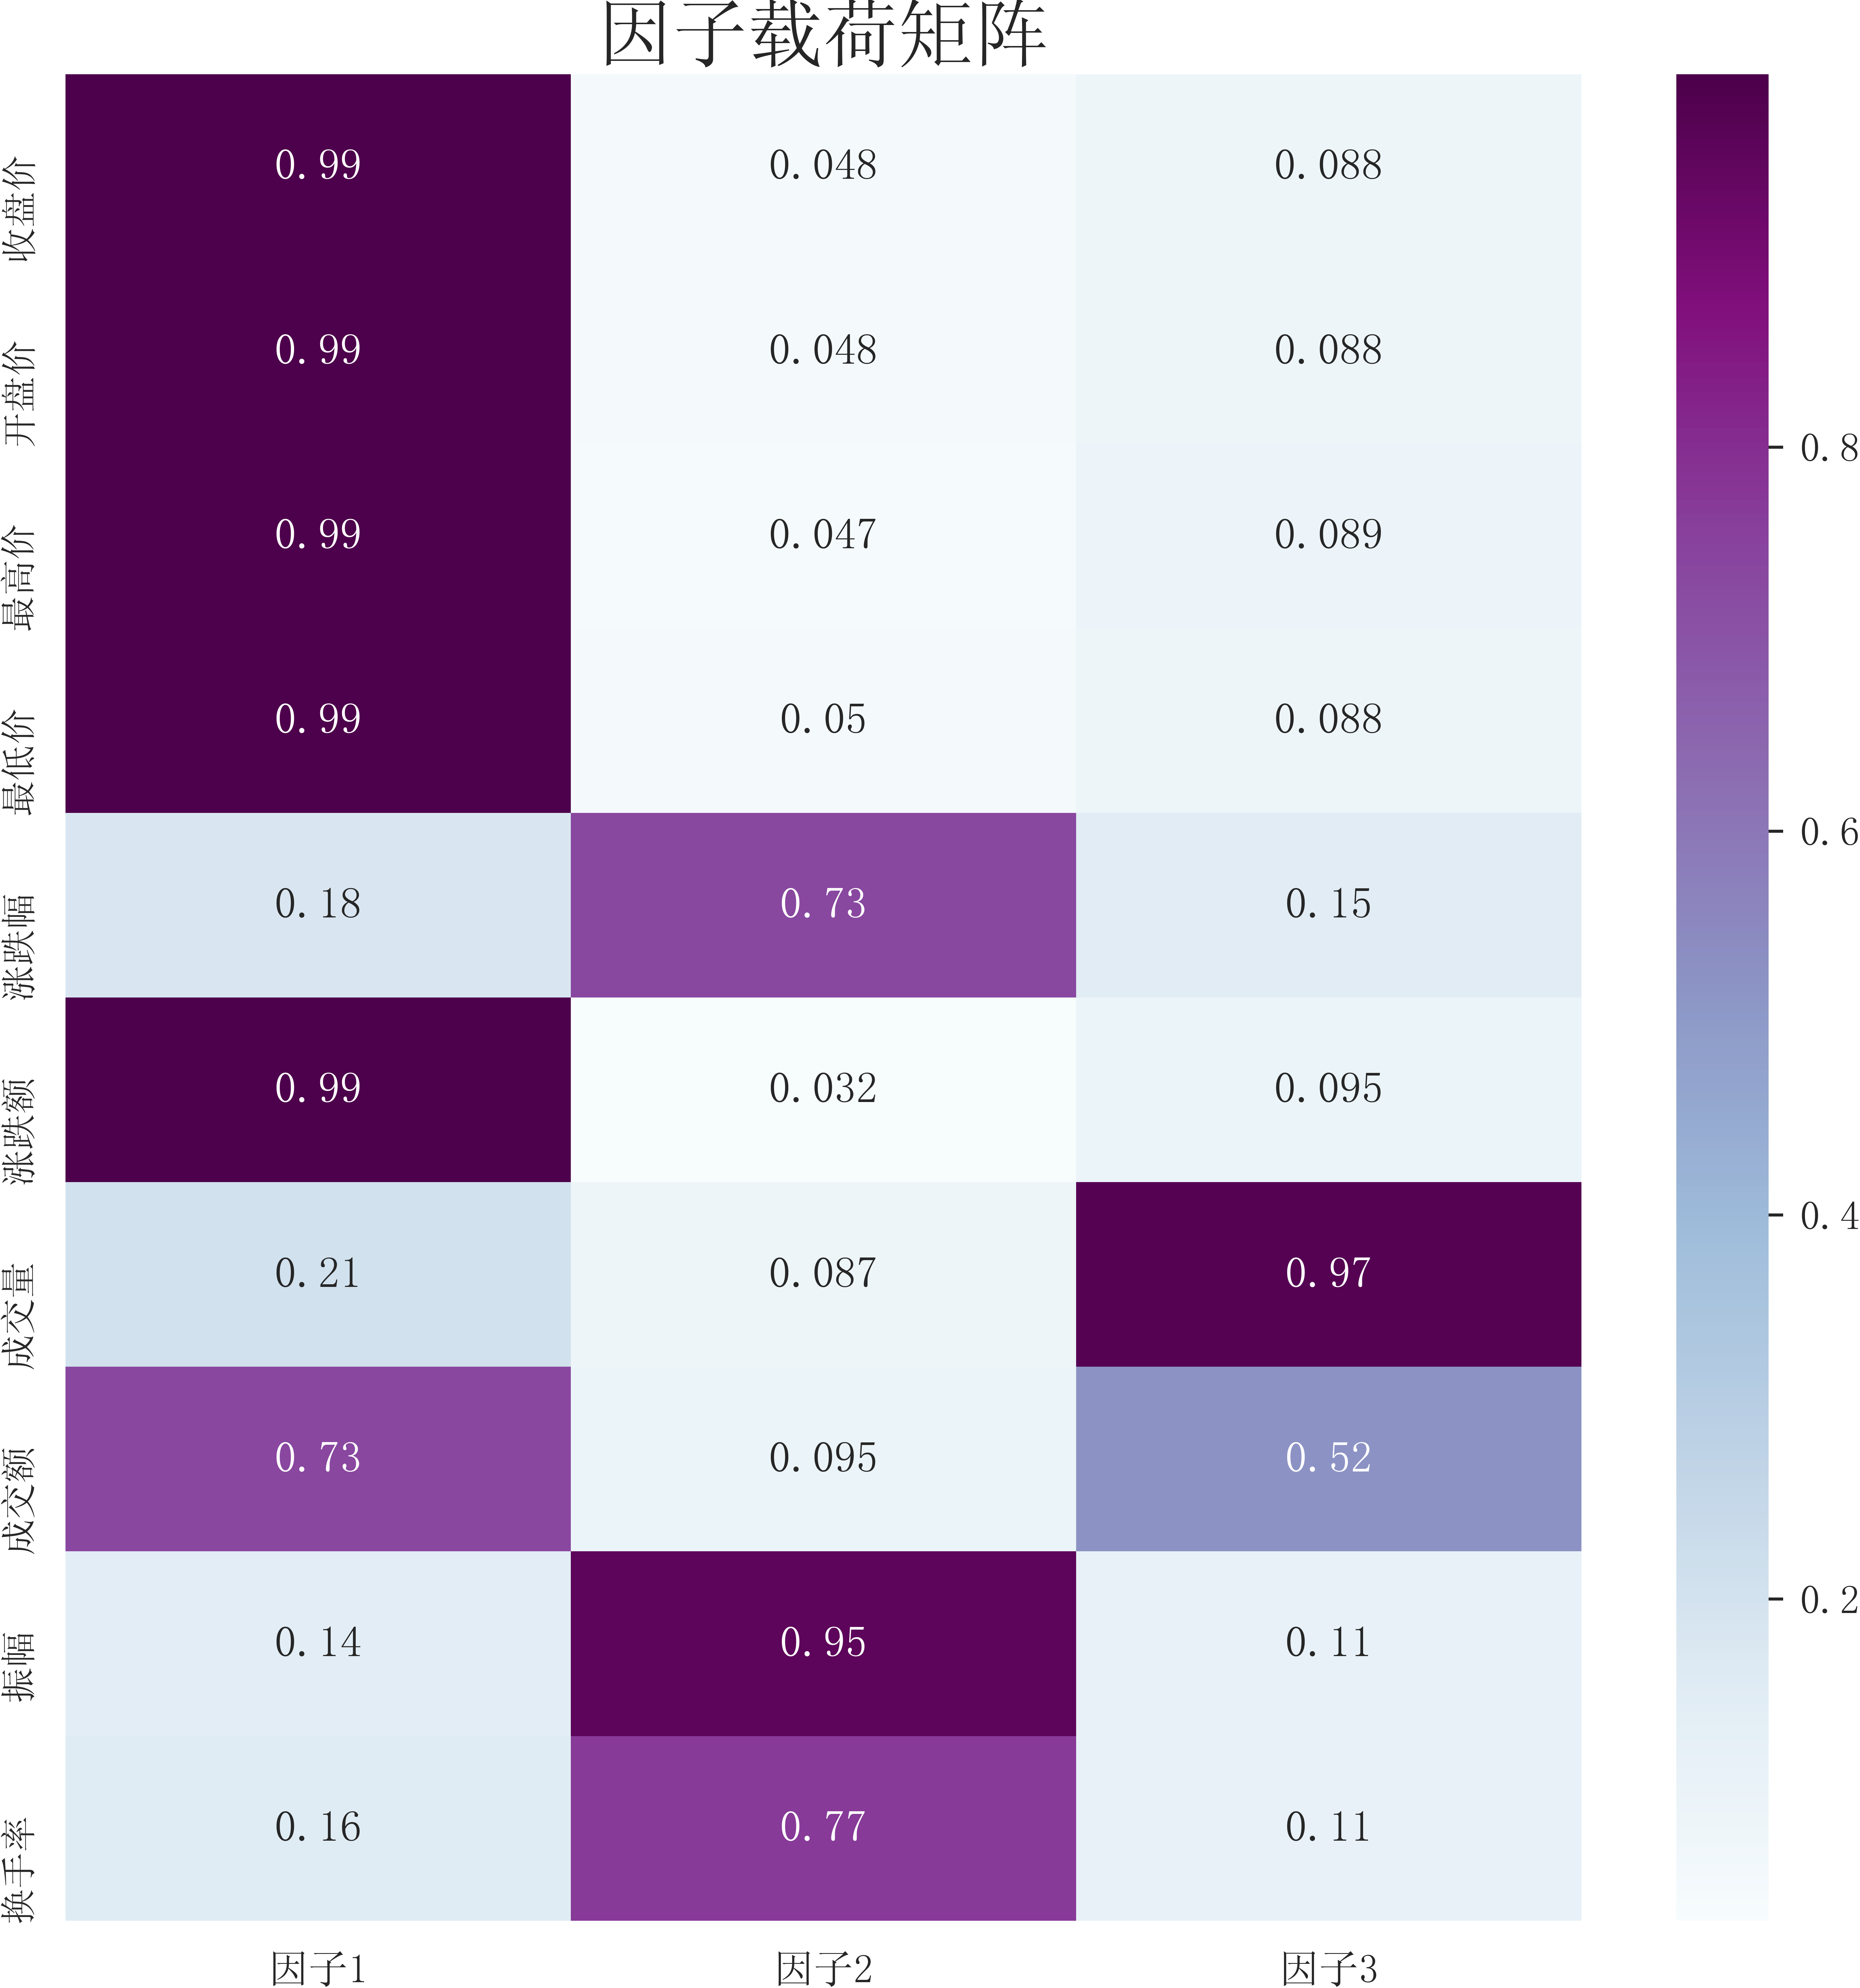
\includegraphics[width=0.7\textwidth]{因子载荷矩阵}
	\caption{因子载荷矩阵}
	\label{因子载荷矩阵}
\end{figure}

第一因子对收盘价、开盘价、最高价、最低价、涨跌额等指标的贡献较大,可以看出这些指标基本都是描述股票的价格情况,因此称第一因子为收益因子;第二主成分对振幅等指标的贡献较大,这部分可以归类为波动情况因子;第三主成分对成交量的贡献比较大,该指标主要描述公司的活跃情况,因此可以称为活跃因子。

对于收益因子和活跃因子来说,往往是越大越好,对波动因子,虽然波动代表了风险,然而波动对于看好短期收益的人来说是一种利好,因此也可以作为一种评分标准。

在得到因子的载荷矩阵之后,通过矩阵运算计算出各个股票的3个因子的得分情况,然后以各个因子对总方差的贡献率为权重,可以加权求和得到各个股票的总得分。在计算出20支股票的得分情况之后,按综合得分倒序排序,列出各股票的因子得分和总得分情况,并作出得分排名条形图。
\begin{table}[htbp]
	\centering
	\caption{因子分析综合得分}
	\begin{tabularx}{\textwidth}{@{}c *4{>{\centering\arraybackslash}X}@{}}
		\toprule[1.5pt]
		\multicolumn{1}{c|}{\textbf{名称}} & \textbf{因子1得分} & \textbf{因子2得分} & \textbf{因子3得分} & \textbf{综合得分} \\
		\midrule
		贵州茅台  & 23.284 & -2.166 & -1.174 & 1.243 \\
		迈瑞医疗  & 2.398 & 0.094 & -1.005 & 0.123 \\
		英科医疗  & -0.738 & 7.646 & -1.259 & 0.101 \\
		片仔癀   & 1.041 & 0.629 & -1.339 & 0.054 \\
		海天味业  & -0.159 & -0.688 & -1.196 & -0.039 \\
		中信证券  & -1.355 & -1.244 & 4.617 & -0.041 \\
		美的集团  & -0.615 & -0.741 & 0.181 & -0.047 \\
		蓝思科技  & -2.023 & 2.044 & 1.449 & -0.052 \\
		恒瑞医药  & -0.480 & -1.453 & 0.290 & -0.053 \\
		格力电器  & -0.805 & -1.578 & 1.342 & -0.060 \\
		海康威视  & -1.263 & 0.017 & 0.729 & -0.061 \\
		爱尔眼科  & -1.310 & 0.680 & -0.347 & -0.064 \\
		华兰生物  & -2.067 & 1.491 & 0.086 & -0.084 \\
		绝味食品  & -1.793 & 1.376 & -1.414 & -0.090 \\
		海螺水泥  & -1.495 & -1.802 & 0.307 & -0.117 \\
		恒顺醋业  & -2.668 & 1.000 & -0.598 & -0.136 \\
		深圳能源  & -2.464 & 0.234 & -0.310 & -0.137 \\
		上汽集团  & -2.265 & -1.444 & 0.599 & -0.149 \\
		白云山   & -2.285 & -2.162 & -0.747 & -0.183 \\
		蓝光发展  & -2.936 & -1.932 & -0.213 & -0.207 \\
		\bottomrule[1.5pt]
	\end{tabularx}%
	\label{因子分析综合得分}%
\end{table}%
		 \begin{figure}[H]
	\centering
	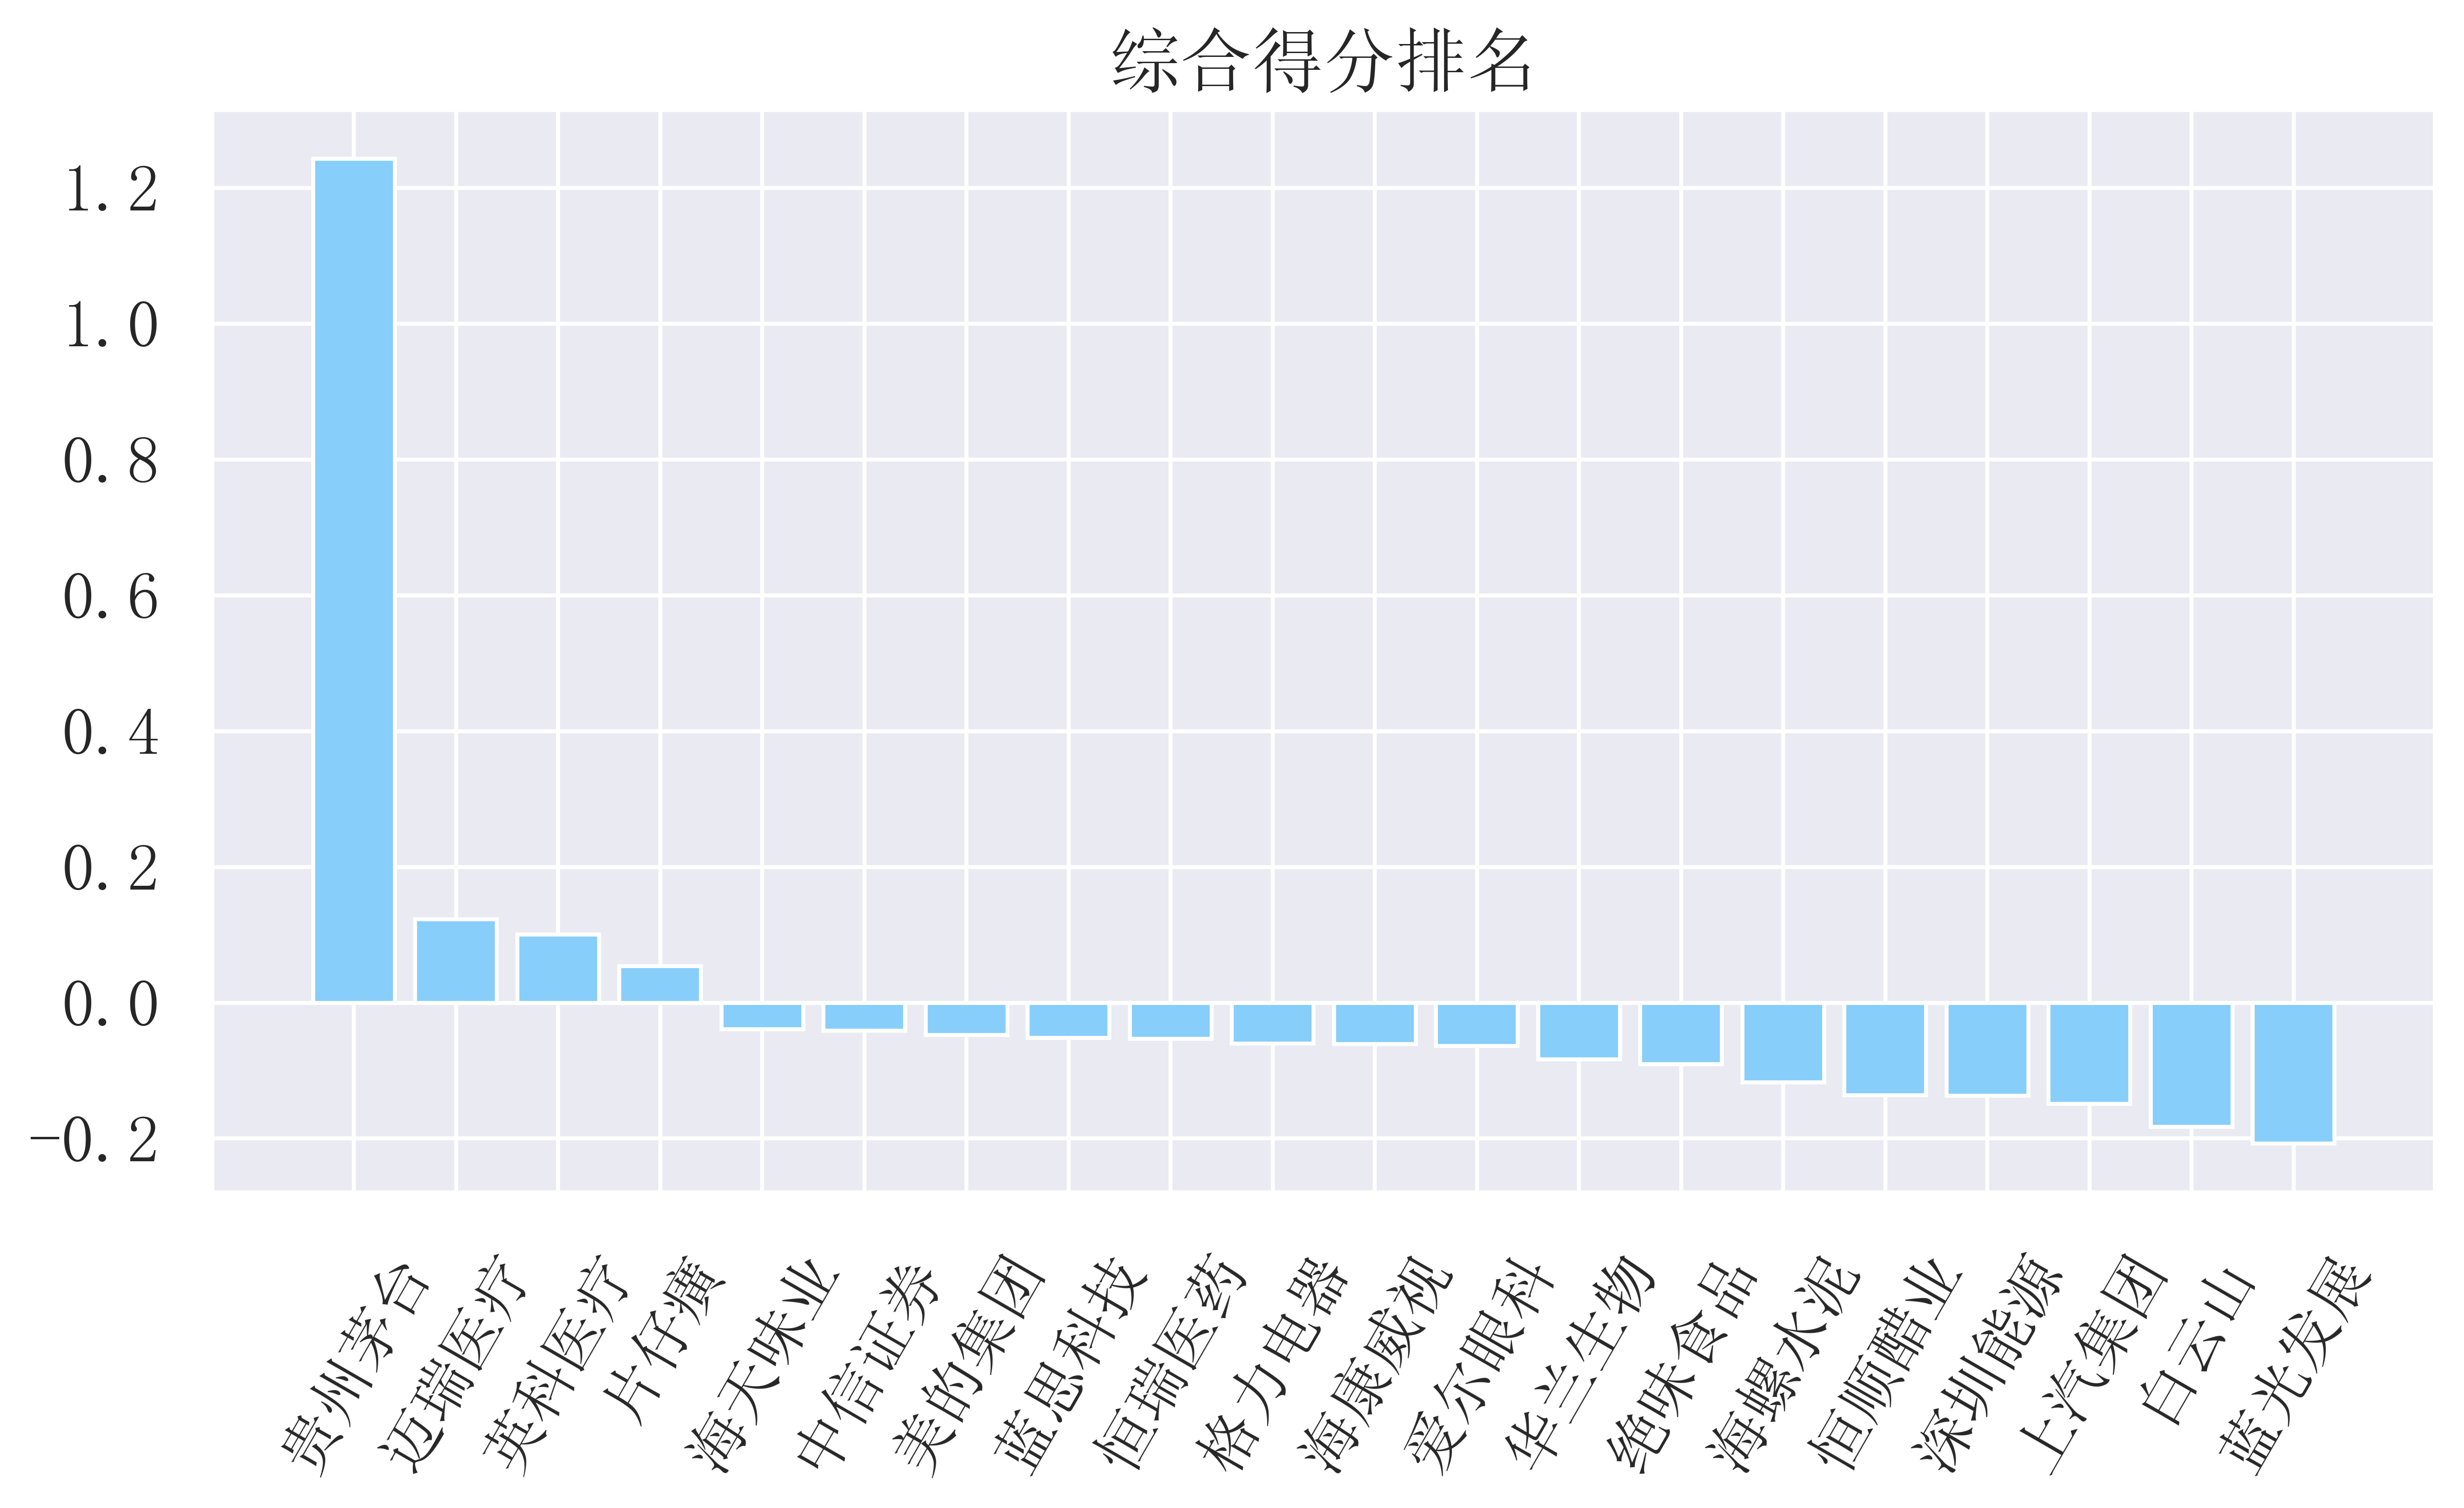
\includegraphics[width=0.7\textwidth]{综合得分排名}
	\caption{综合得分排名}
	\label{综合得分排名}
\end{figure}
主成分得分综合体现了股票近期的成长能力、盈利能力、活跃能力。得分越高,说明股票预期收益越来越好,值得买入;反之,则说明股票近期状况比较低迷,即收益不好,波动也不足,对于长期投资和短期投资的人都不利,投资有较大的风险。

因此,可以从排名结果中选取贵州茅台、迈瑞医疗、英科医疗、片仔癀、海天味业五支股票作为最具潜力股票。
	
	\subsection{正态性检验}	
JB统计量全称叫Jarque-Bera统计量,是用来检验一组样本是否能够认为来自正态总体的一种方法\upcite{wuJunZhiYuPianDuYueShuXiaCVaRZuiXiaoTouZiZuHeYouHuaMoXingYanJiu2014}。

首先计算偏度系数S:
$$
S=\frac{\sum\left(x_{t}-\bar{x}\right)^{3}}{n \sigma^{3}}
$$
及峰度系数K:
$$
K=\frac{\sum\left(x_{t}-\bar{x}\right)^{4}}{n \cdot \sigma^{4}}
$$
对于正态分布变量,偏度为零,峰度为3.
Jarque和Bera建立了如下检验统计量JB统计量:
$$
J B=\frac{n}{6}\left[S^{2}+\frac{(K-3)^{2}}{4}\right]
$$
其中,n为样本容量,S为偏度,K为峰度。在正态分布的假设下,JB统计量渐进地服从自由度为2的卡方分布,$\text { JBasy } \sim \chi 2(2)$若变量服从正态分布,则S为零,K为3,因而JB统计量的值为零
如果JB统计量值较大,则不能认为样本来自正态分布。

利用Python软件编程对20只股票的收益率序列进行正态分布检验,计算JB统计量及对应的P值、偏度、峰度如表\ref{各股票的JB统计量P值偏度和峰度}.

% Table generated by Excel2LaTeX from sheet 'Sheet1'
\begin{table}[htbp]
	\centering
	\caption{各股票的JB统计量,P值,偏度和峰度}
	\begin{tabularx}{\textwidth}{@{}c *4{>{\centering\arraybackslash}X}@{}}
		\toprule
		\textbf{名称} & \textbf{JB统计量} & \textbf{P值} & \textbf{偏度S} & \textbf{峰度K} \\
		\midrule
		迈瑞医疗  & 4.61  & 0.10  & -0.28 & 3.38 \\
		片仔癀   & 35.79 & 0.00  & 0.04  & 4.88 \\
		爱尔眼科  & 19.17 & 0.00  & -0.23 & 4.29 \\
		贵州茅台  & 45.80 & 0.00  & -0.45 & 4.93 \\
		恒瑞医药  & 69.96 & 0.00  & 0.21  & 5.59 \\
		海天味业  & 43.23 & 0.00  & -0.10 & 5.06 \\
		格力电器  & 12.00 & 0.00  & 0.33  & 3.87 \\
		美的集团  & 20.31 & 0.00  & -0.13 & 4.39 \\
		海螺水泥  & 249.66 & 0.00  & 1.29  & 7.24 \\
		恒顺醋业  & 8.05  & 0.02  & 0.16  & 3.83 \\
		绝味食品  & 3.49  & 0.17  & 0.19  & 3.45 \\
		白云山   & 302.19 & 0.00  & 0.77  & 8.24 \\
		华兰生物  & 7.80  & 0.02  & 0.15  & 3.83 \\
		深圳能源  & 205.91 & 0.00  & 1.17  & 6.85 \\
		中信证券  & 275.53 & 0.00  & 1.01  & 7.81 \\
		蓝光发展  & 251.67 & 0.00  & 0.98  & 7.58 \\
		海康威视  & 33.66 & 0.00  & 0.45  & 4.58 \\
		英科医疗  & 13.21 & 0.00  & 0.25  & 4.03 \\
		上汽集团  & 78.58 & 0.00  & 0.76  & 5.33 \\
		蓝思科技  & 12.57 & 0.00  & 0.29  & 3.95 \\
		\bottomrule
	\end{tabularx}%
	\label{各股票的JB统计量P值偏度和峰度}%
\end{table}%
并给出4只股票的QQ 图以便更加直观的判断正态检验的结果。
\begin{figure}[H]
	\centering
	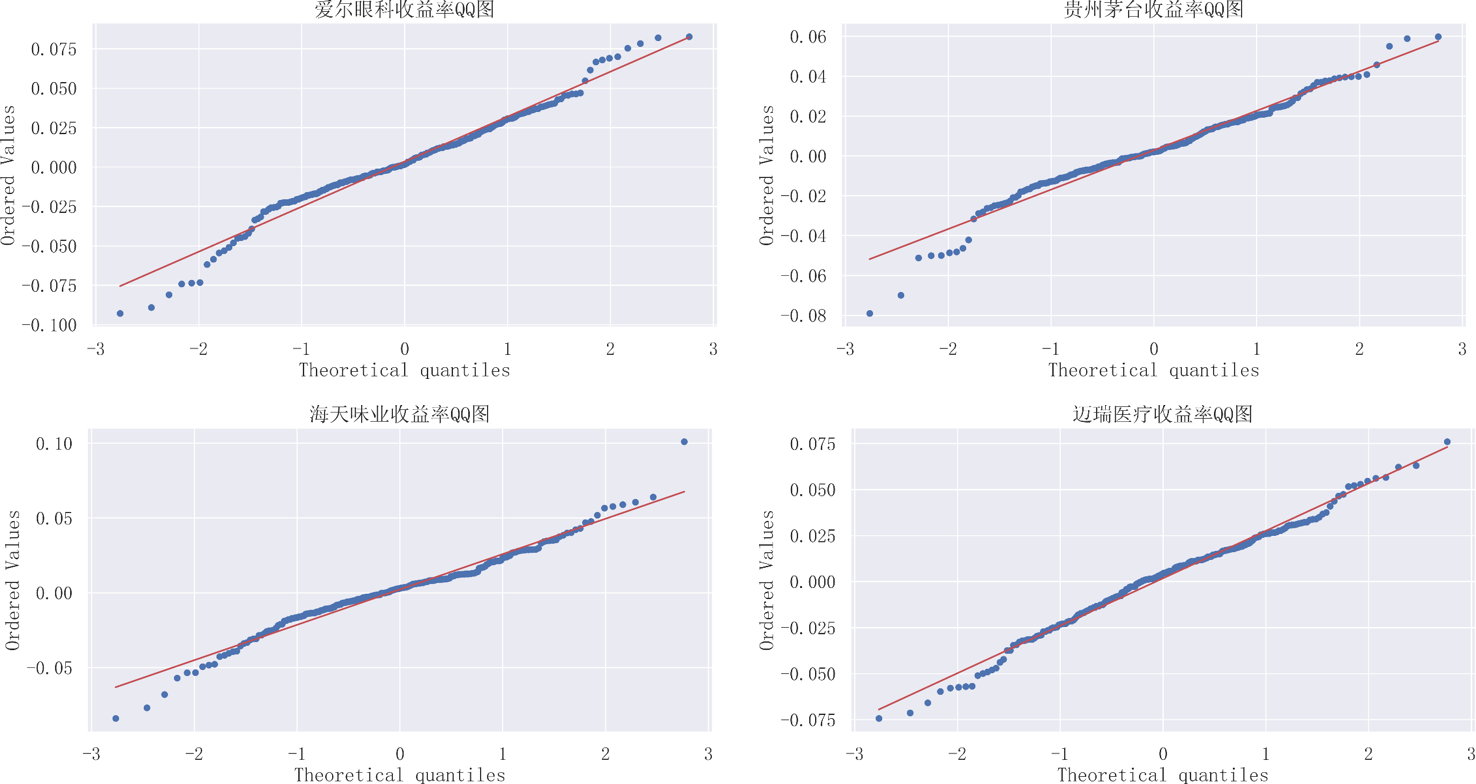
\includegraphics[width=0.75\textwidth]{QQ图组合}
	\caption{部分股票收益率QQ图}
	\label{部分股票收益率QQ图}
\end{figure}
从表和图中的检验结果表明20只股票的收益率序列有少部分近似服从正态分布,表现为JB统计量较小,而大部分股票的JB统计量较大,不服从正态分布,部分股票的收益率向量更是存在尖峰厚尾、波动集聚的特征。为此,本文在后续的研究中不采用方差-协方差方法进行建模,而采用历史模拟法来规避正态性假设所产生的误差。
	\subsection{投资组合方案}	
	\subsubsection{均值-方差模型}
	对于优化模型(\ref{model1}),需要利用合适的算法进行求解。为求解出最优投资方案,每只股票的平均收益率、每只股票的方差以及协方差矩阵。
	\begin{equation}
	\begin{array}{ll}
	\min & \lambda\left[\sum_{i=1}^{N} \sum_{j=1}^{N} x_{i} x_{j} \sigma_{i j}\right]-(1-\lambda)\left[\sum_{i=1}^{N} x_{i} \mu_{i}\right] \\
	\text { s.t. } & \sum_{i=1}^{N} x_{i}=1 \\
	& 0 \leq x_{i} \leq 1 \\
	& i=1, \ldots, N
	\end{array}
	\label{model1}
	\end{equation}

由协方差矩阵计算公式计算20只股票的协方差:
$$
\sigma(x, y)=\frac{1}{n-1} \sum_{i=1}^{n}\left(x_{i}-\bar{x}\right)\left(y_{i}-\bar{y}\right)
$$
当协方差的绝对值越大时,每支股票的波动就越大,风险也
就越大。为了使风险能进一步降低,我们需要在制定投资策略中使得协方差进一步降低。

本文首先采用蒙特卡洛模拟来进行分析,随机生成一组权重,计算该组合下的收益和标准差,重复这一过程许多次,将每一种组合的收益和标准差绘制成散点图,并以对应的夏普比率加以颜色,并找出图中的方差最小及收益最大的两个点,这两个点即对应最小方差模型和最大收益模型。
	\begin{figure}[H]
	\centering
	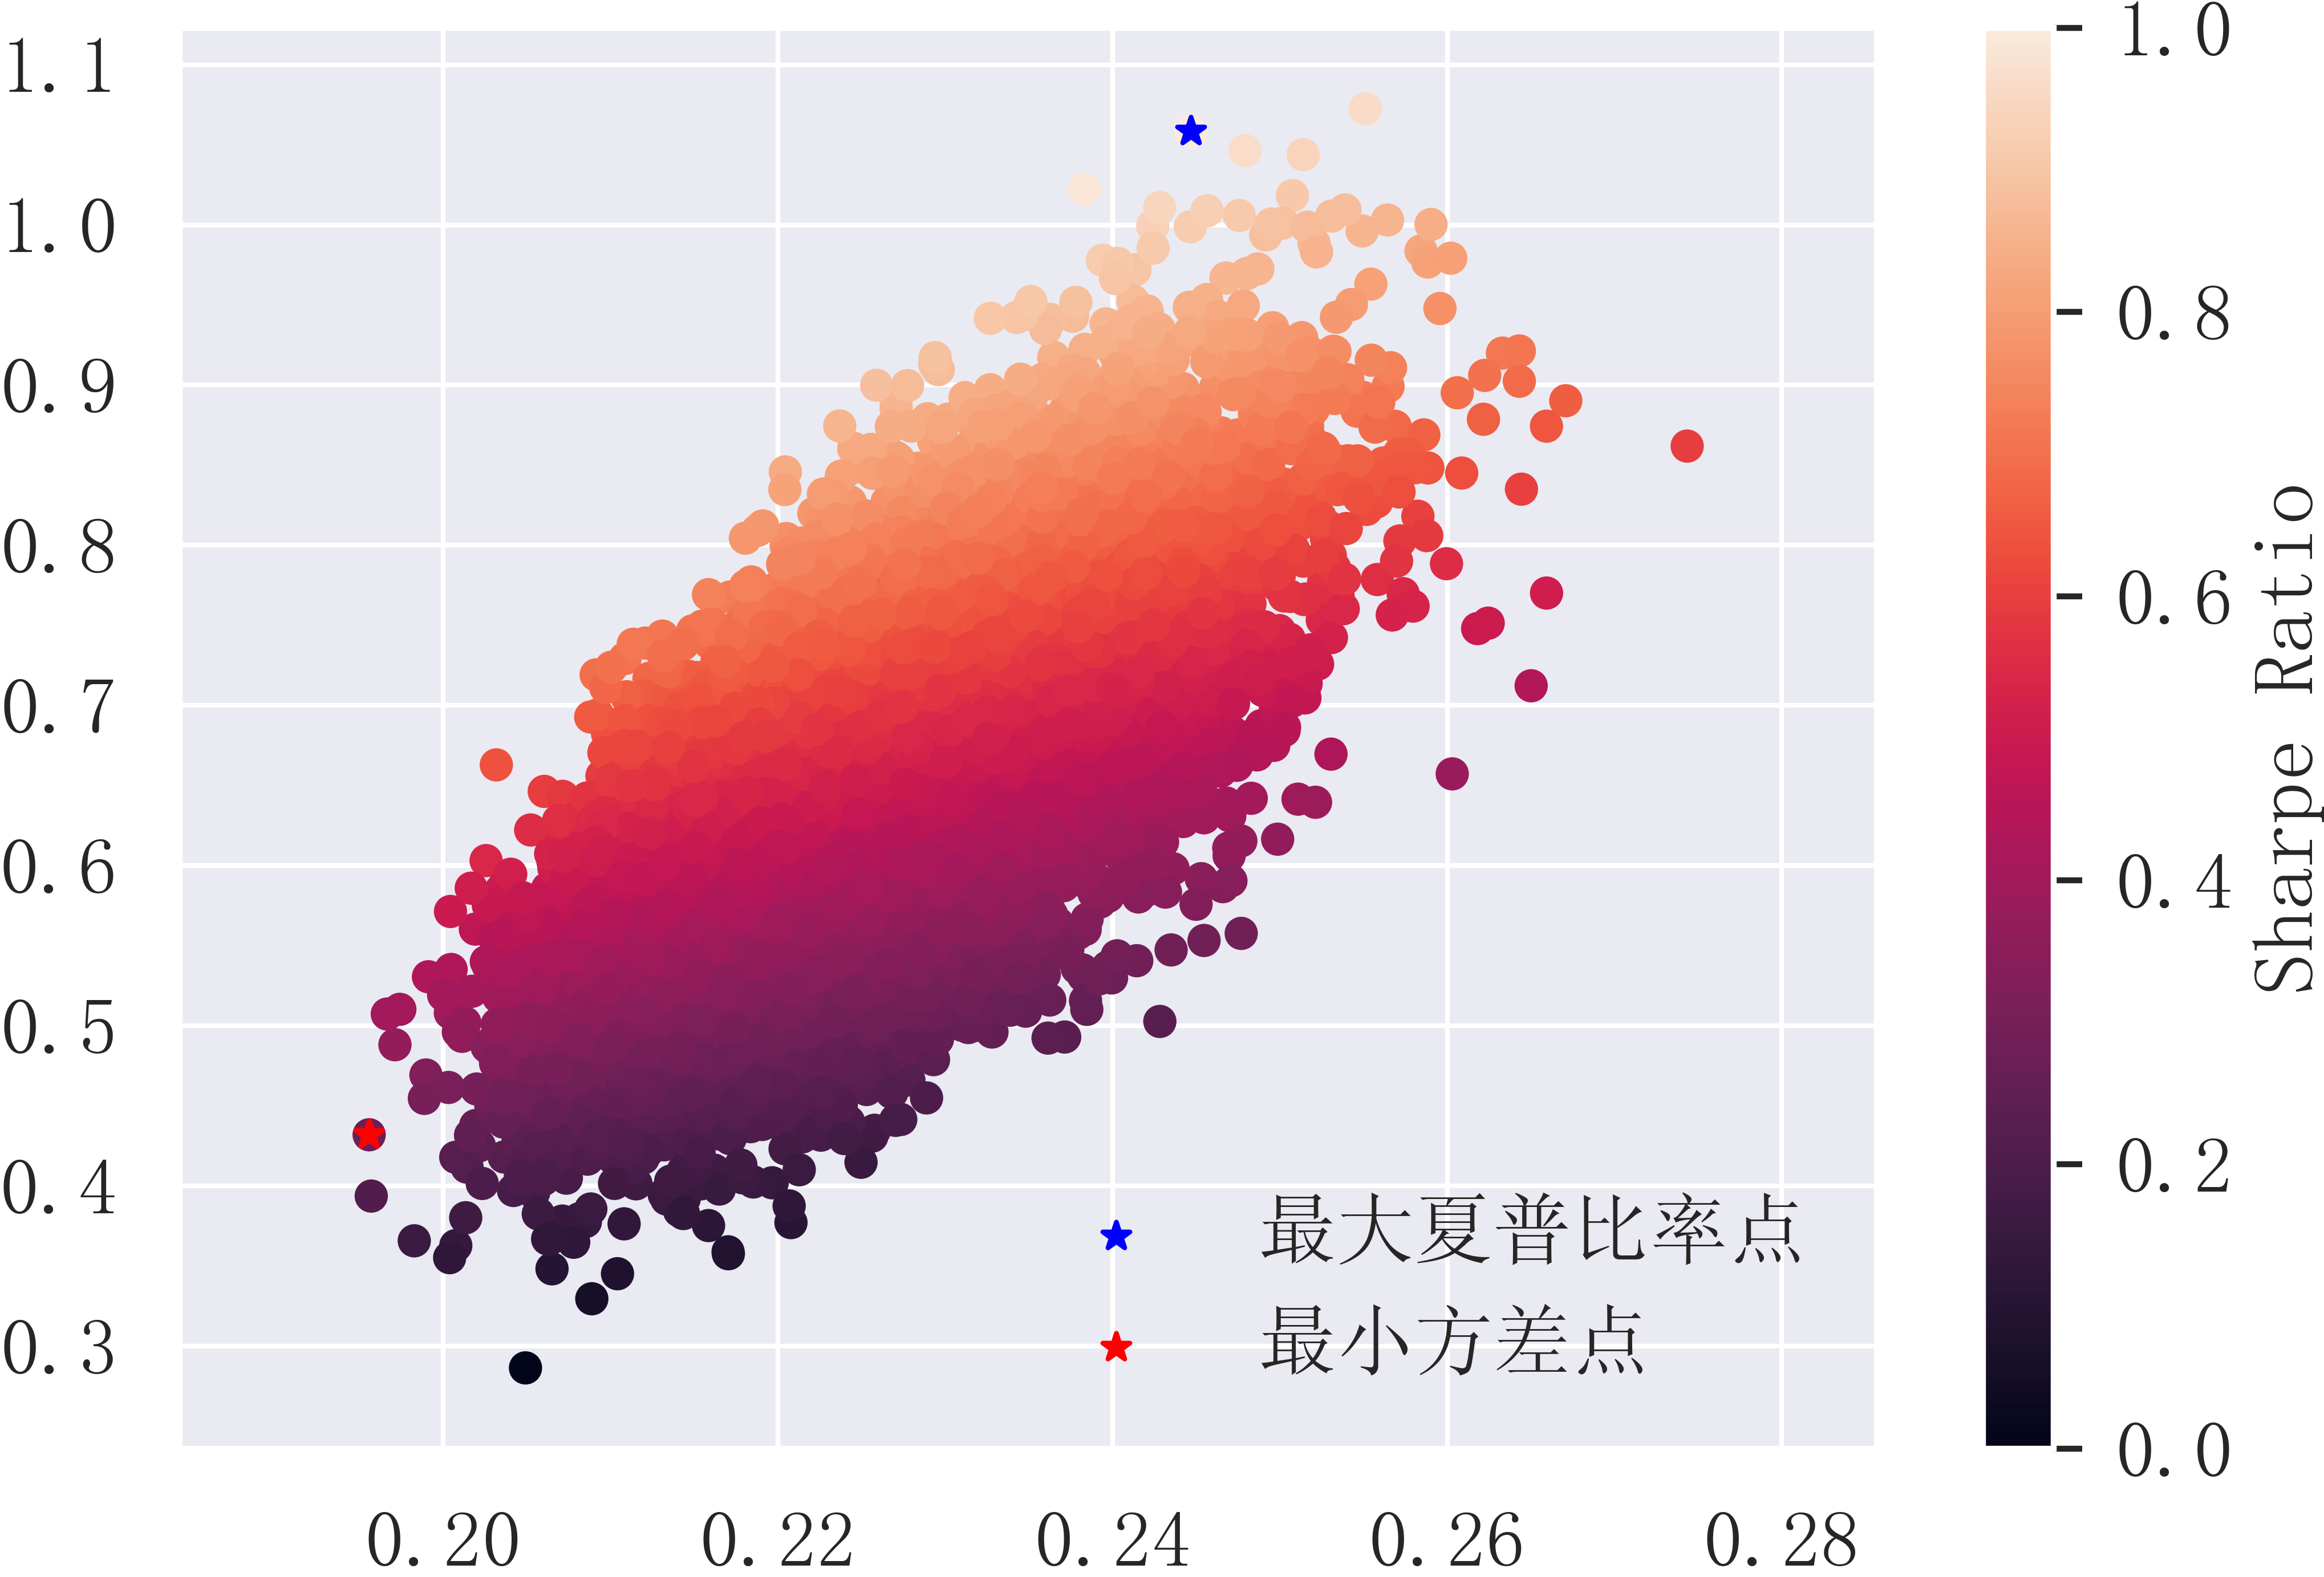
\includegraphics[width=0.7\textwidth]{夏普比率图}
	\caption{蒙特卡洛模拟}
	\label{蒙特卡洛模拟}
\end{figure}
上述蒙特卡洛模拟方法求得的方差最小点和收益最大点只是局部最优解,要想求得全局最优,只能利用精确求解的方法。利用Python软件精确求解多目标规划模型,求得的结果即构成了均值方差模型的有效前沿,作出有效前沿,并标记最小方差点、最大收益点及最大夏普比率点。
	\begin{figure}[H]
	\centering
	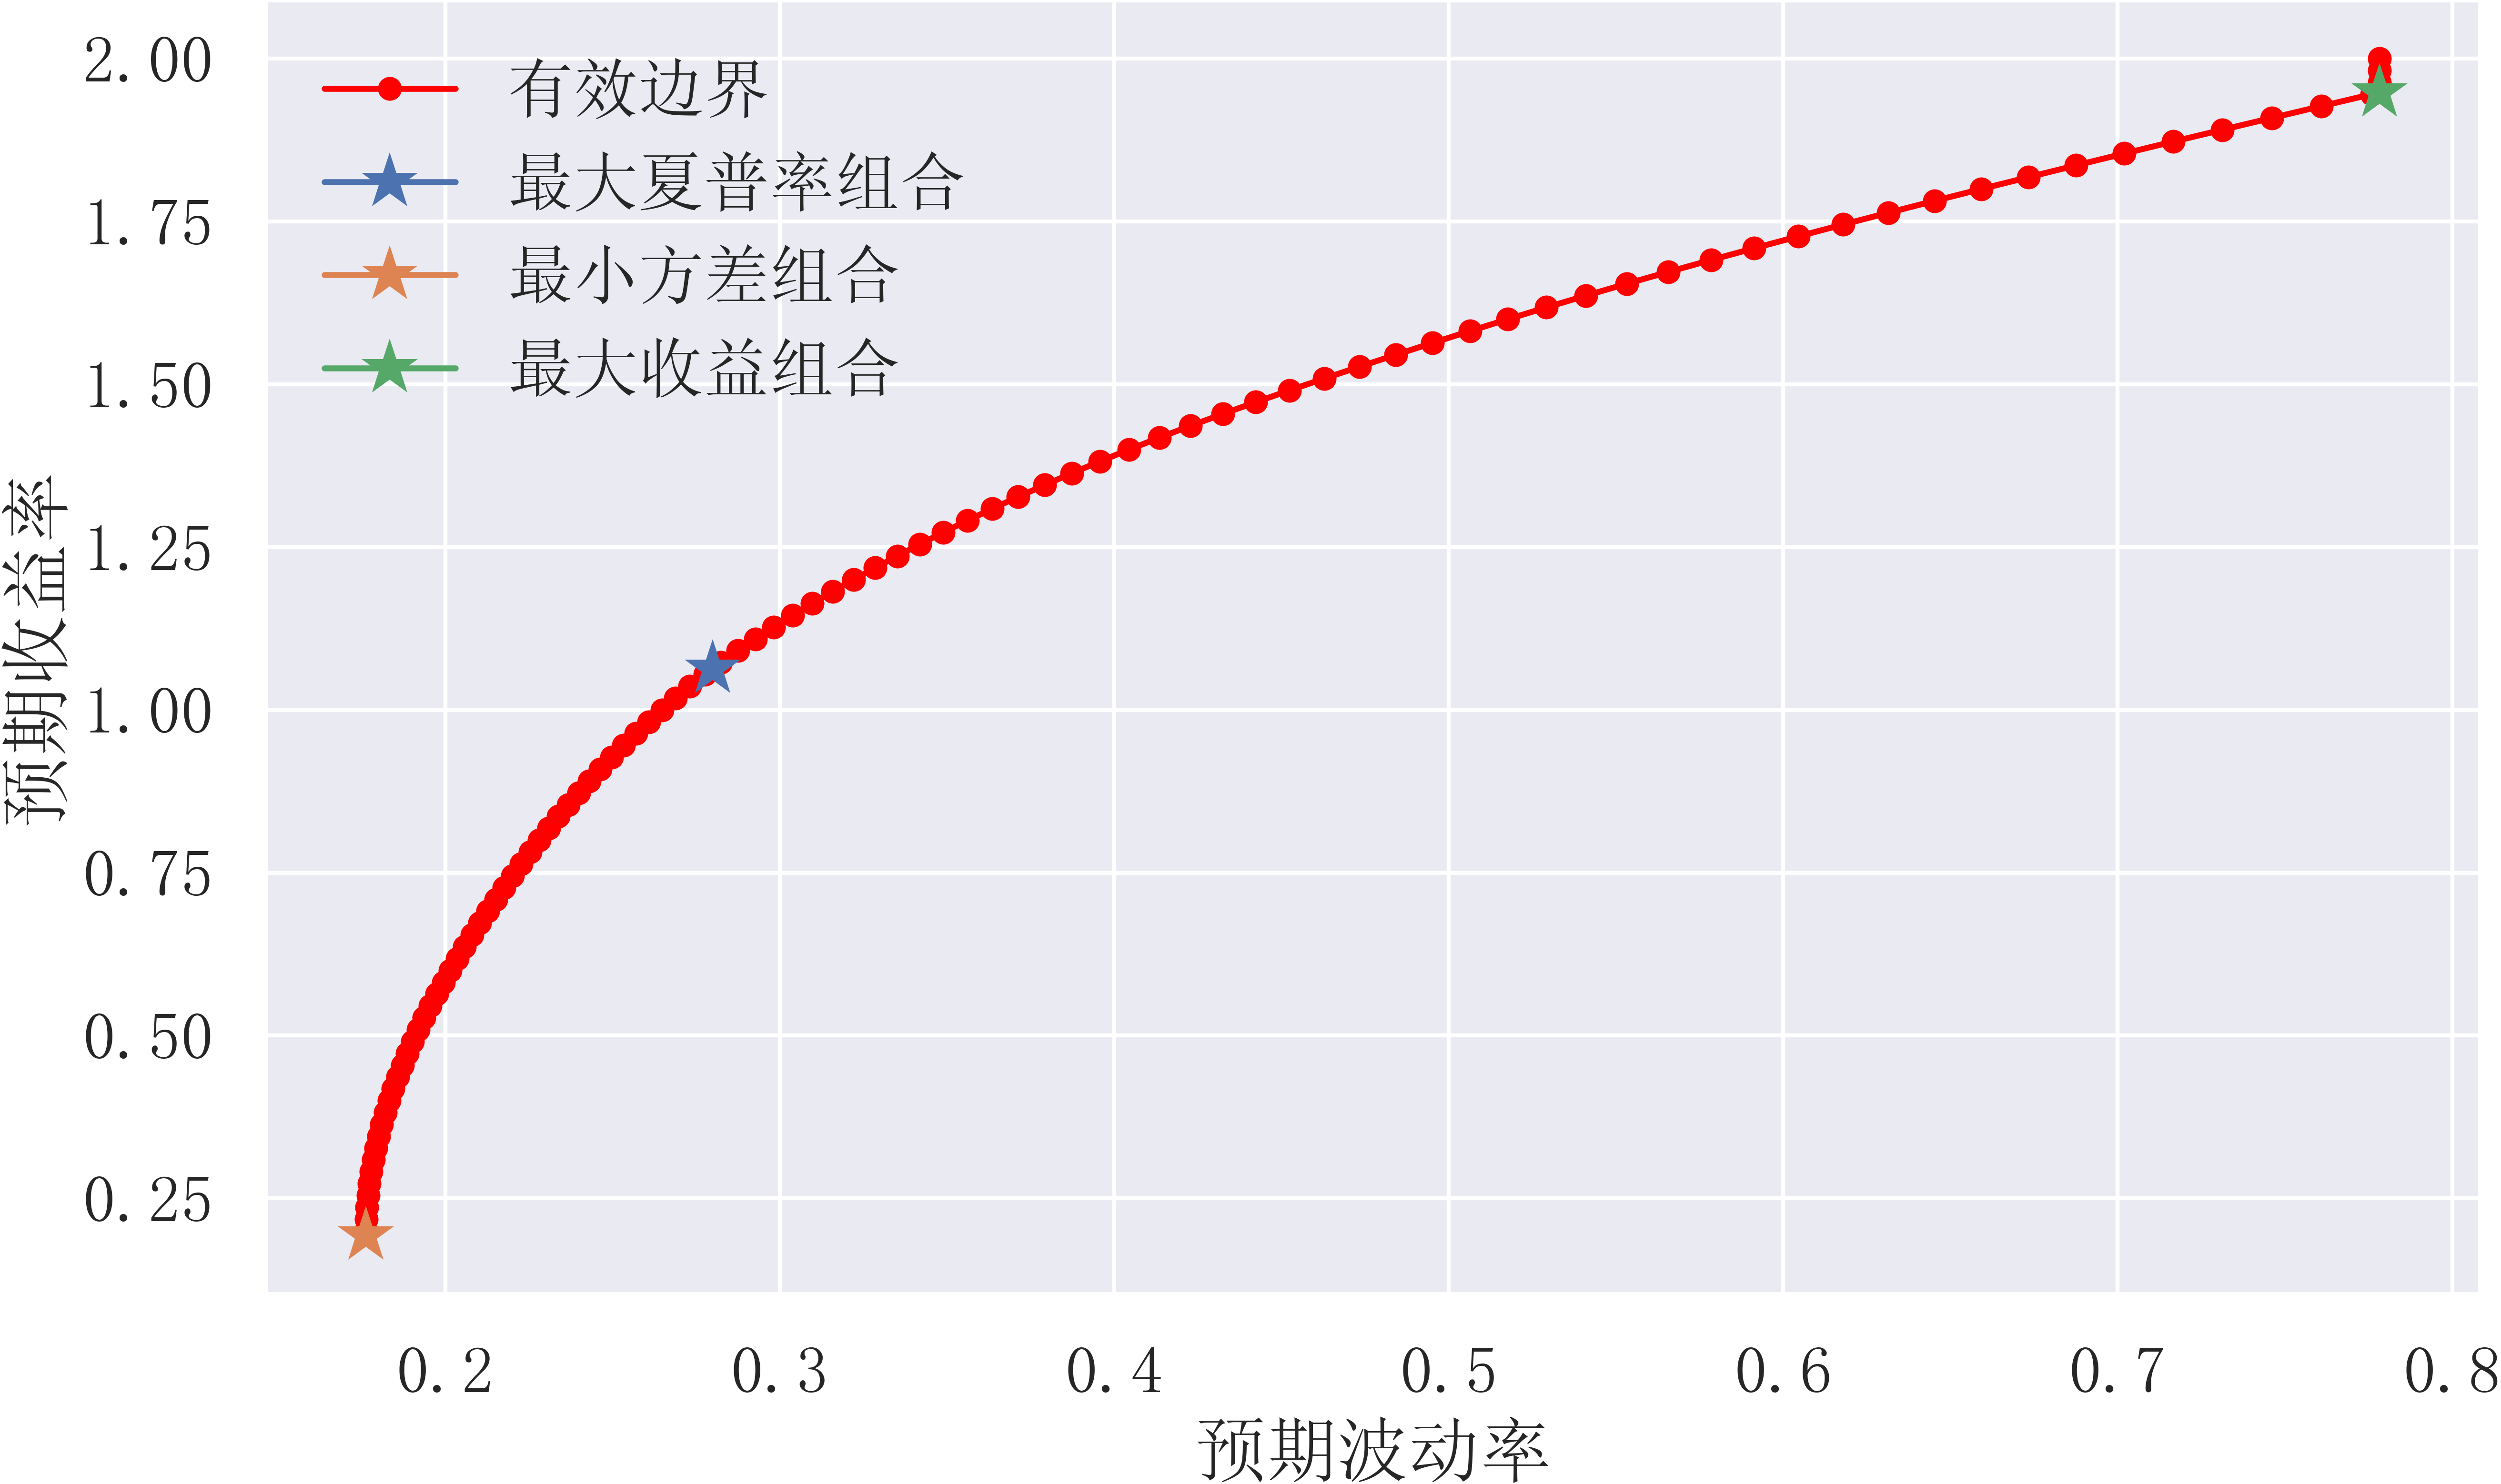
\includegraphics[width=0.7\textwidth]{mean-方差模型有效边界}
	\caption{均值-方差模型有效边界}
	\label{mean-方差模型有效边界}
\end{figure}
均值方差模型3种情形下的股票分配如下:
	\begin{figure}[H]
	\centering
	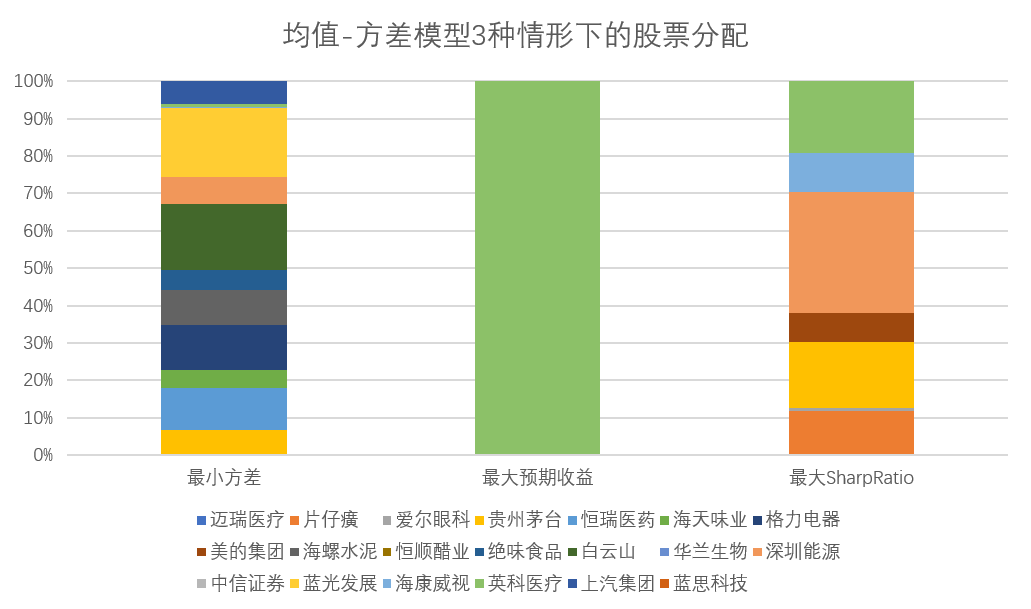
\includegraphics[width=0.85\textwidth]{均值方差模型3种情形下的股票分配}
	\caption{均值方差模型3种情形下的股票分配}
	\label{均值方差模型3种情形下的股票分配}
\end{figure}
我们看到,最厌恶风险的投资组合(即方差最小模型)主要由多种股票组成,平均每种股票的分配较少,体现了分散投资分散风险的思想。随着风险水平的提高,股票数量减少,股票分配会增加。对于收益最大模型,则完全投资一种股票,该股票即收益率最大的股票,然而,对应的风险也是最大的。而对于夏普比率最大模型,股票数量介于两者之间,投资比例相对均衡,在实际的操作中,我们往往也是选择夏普比率最大模型对于的投资组合。

	\subsubsection{均值-CVaR模型}
	均值-CVaR模型的求解同上面的均值-方差模型求解过程一样,所不同的是均值-CVaR模求解的是式(\ref{model2})
	\begin{equation}
	\begin{aligned}
	&\max \frac{E\left(R_{p}\right)-R_{f}}{\hat{F}_{a}(x, \theta)} \\
	&\text { s.t }\left\{\begin{array}{l}
	\hat{E}\left(R_{p}\right)=x^{T} \bar{R} \geq r_{0} \\
	\theta+\frac{1}{J(1-\alpha)} \sum_{k=1}^{J} d_{k} \leq W_{0} \\
	d_{k} \geq-x^{T} R^{k}-\theta \\
	d_{k} \geq 0 \\
	\sum_{i=1}^{n} x_{i}=1 \\
	0 \leq x_{i} \leq 1
	\end{array}\right.
	\end{aligned}
	\label{model2}
	\end{equation}
	求解上式涉及到置信水平的选择:本文将讨论不同置信水平下的模型求解问题,置信水平从一定程度上反映了投资者本身对风险的主观程度,如果是风险偏好者,可采用90\%的置信水平;风险中立者,则为95\%的置信水平;而风险规避者,可选择最为谨慎的99\%置信水平。需要说明的是,当置信水平越高的时候,损失超过 CVaR 的可能性越小,需要的数据就越多,才能体现出好的预测效果,所以往往在实际中无法获取大量数据,这就抑制了较高置信水平的选择。
	
	对选定的股票,均值-方差模型只能给出一组最优的投资组合,而基于均值-CVaR 的投资组合优化模型则不同,其投资组合的有效前沿是滑动的,不同的置信水平确定着不同有效的投资组合前沿面。
	
	将置信水平设置为90\%,95\%和99\%,即$\alpha=0.1,0.05,0.01$,分别代入式(\ref{model2})求解,并绘制有效前沿:
		\begin{figure}[H]
		\centering
		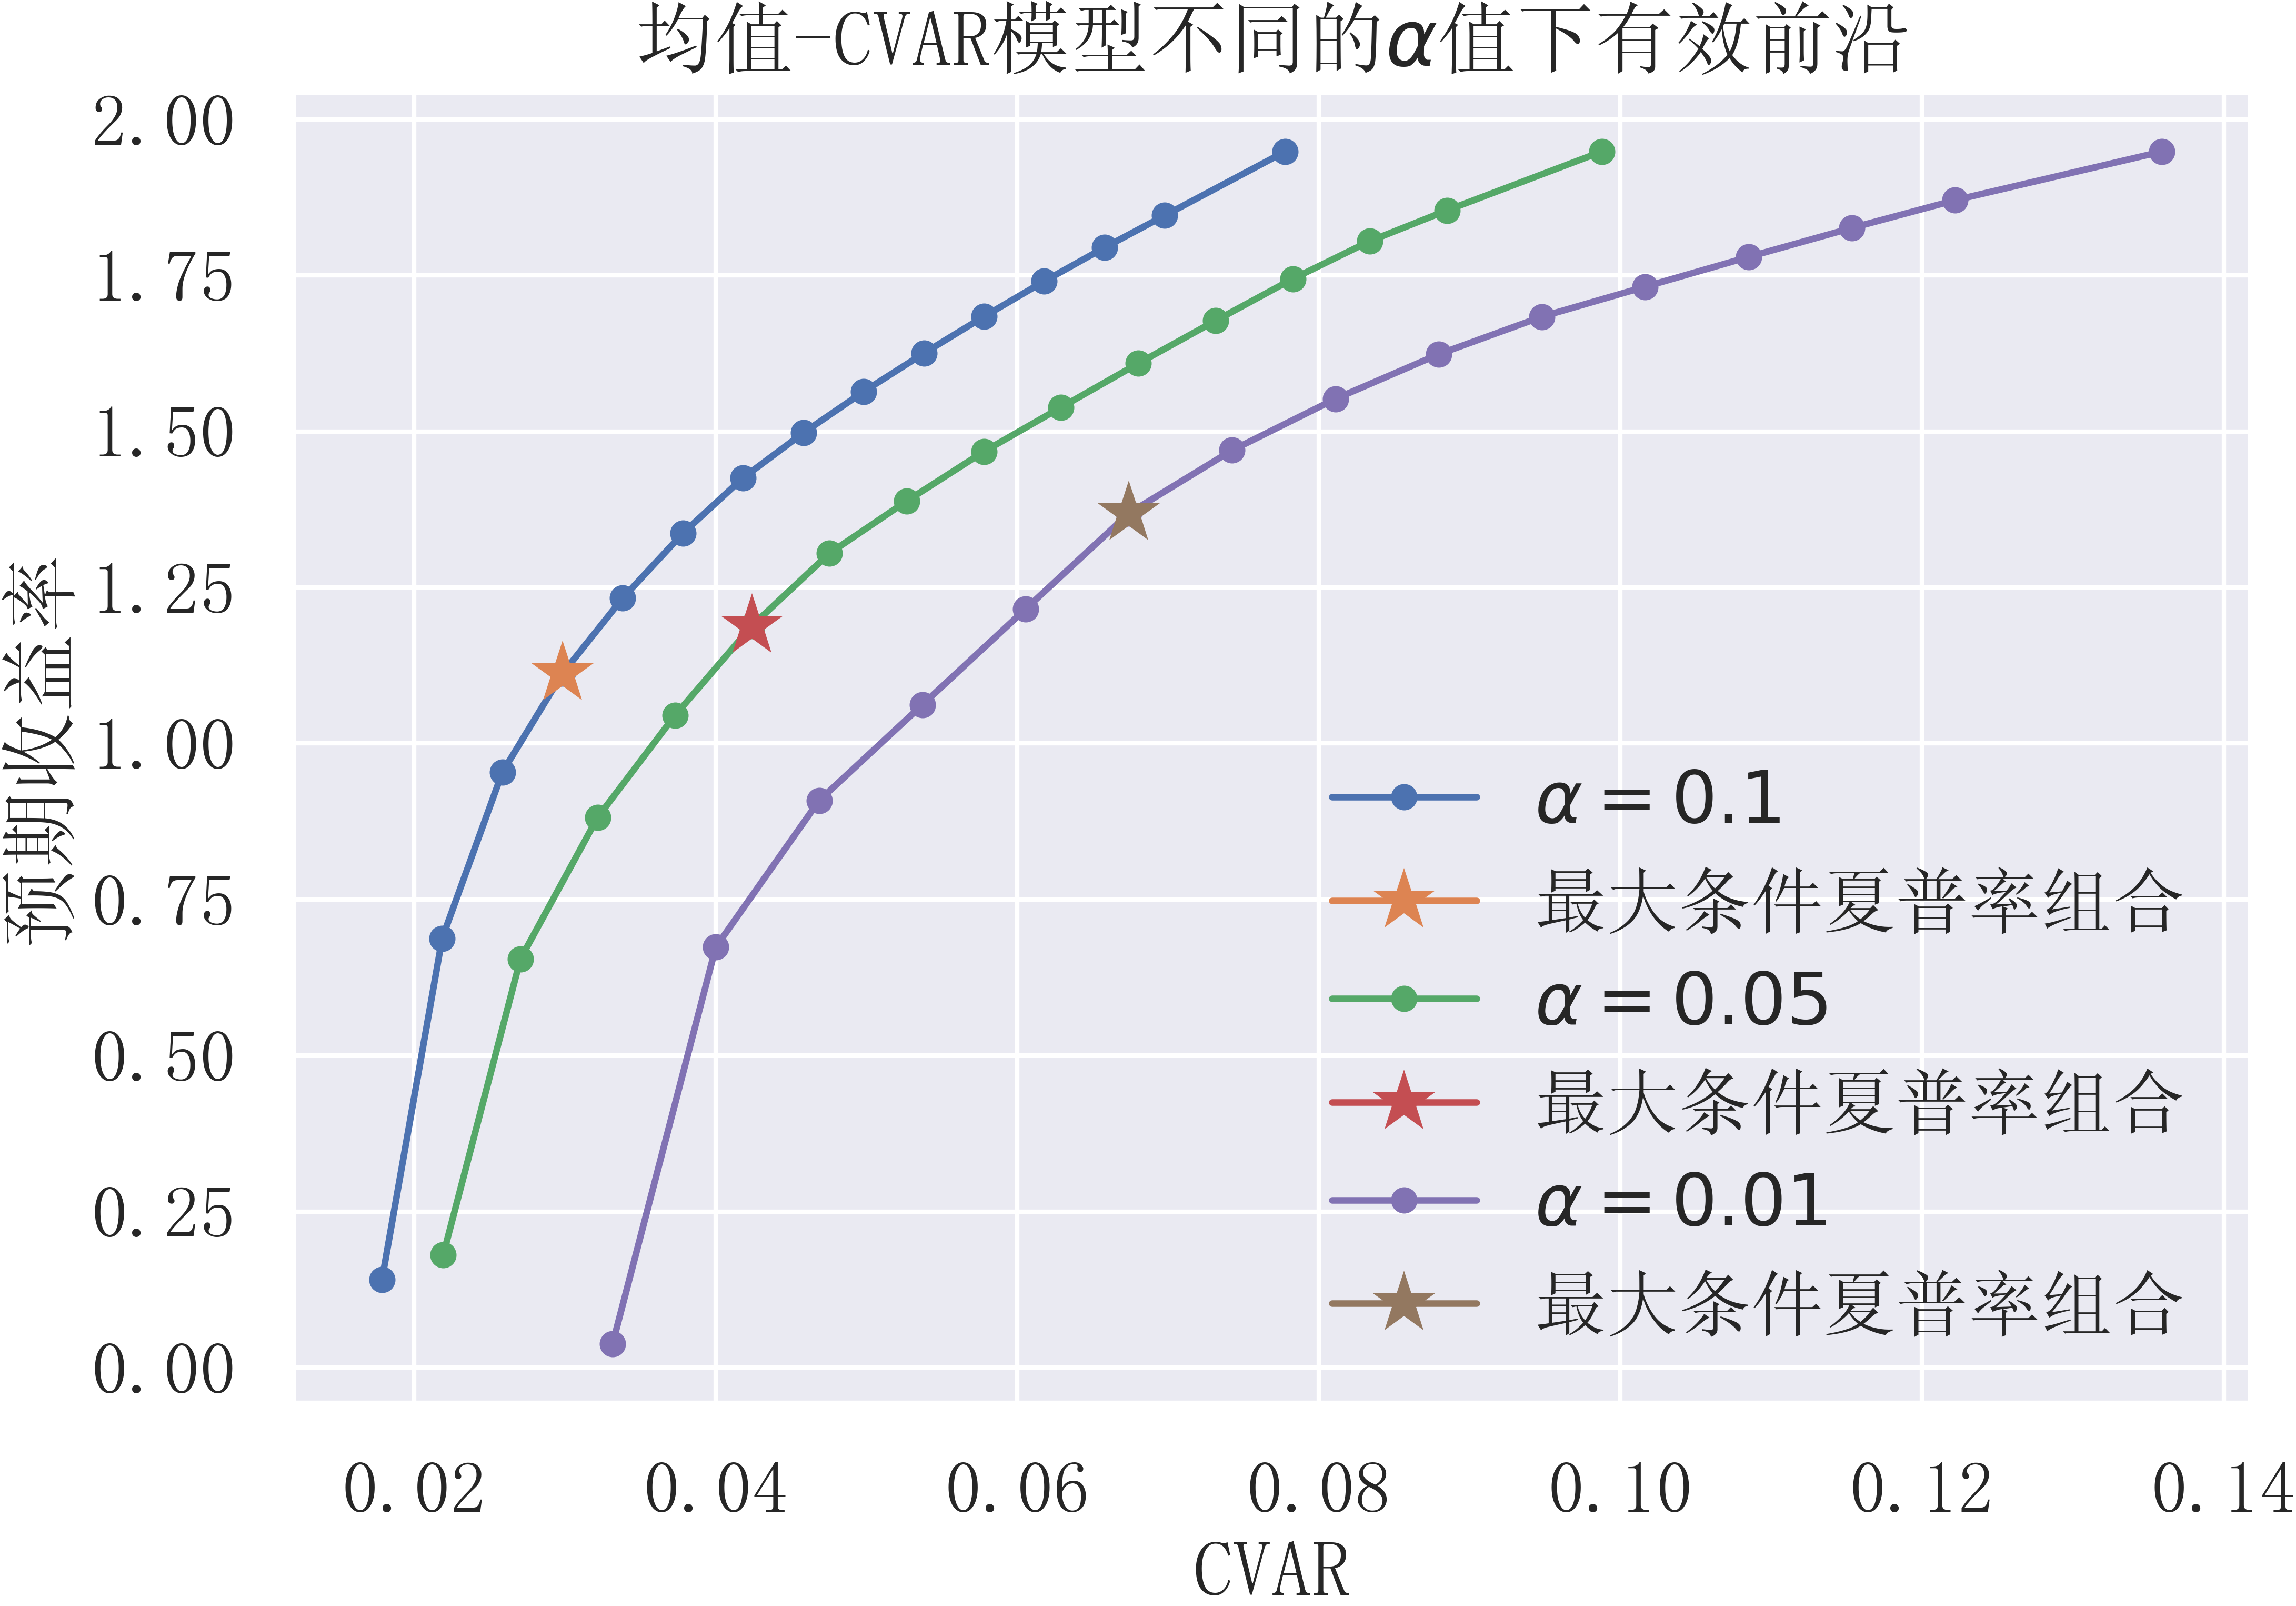
\includegraphics[width=0.7\textwidth]{均值-CVAR模型不同的alpha值下有效前沿}
		\caption{均值-CVAR模型不同的$\alpha$值下有效前沿}
		\label{均值-CVAR模型不同的alpha值下有效前沿}
	\end{figure}
由上图可以清晰的看出,随着置信水平的变化,由其所确定的有效前沿差异
显著,呈现下列特征:

第一,随着置信水平的变大,有效前沿右移,可行集也随之右移,投资组合
的收益率区间也在收窄;在收益率相同的情况下,对应的CVaR 值也在不断的变大。
当投资者预期的组合收益率增时,CVaR 的值也越来越高,说明投资者所承受的风
险也越来越大,这也说明风险与收益之间是密不可分的。如果投资者是厌恶风险
的,那么通过提高置信水平降低损失风险发生的概率时,相应的组合收益也随之
下降。总之,均值-CVaR 模型所展现出的风险收益关系同样满足高风险高收益的
特征。

第二,投资者在根据自身的风险偏好及风险承受能力确定的情况下,CVaR 值
会随着预期的组合收益率的增加而增大。投资者的目标CVaR 值越大,投资组合将
更多的集中于部分高收益的股票;反之,投资组合中的股票越分散。同样地,在
投资者确定了目标组合收益率的情况下,随着置信水平选择的增大,其资金对于
股票的配置越集中.
		\begin{figure}[H]
	\centering
	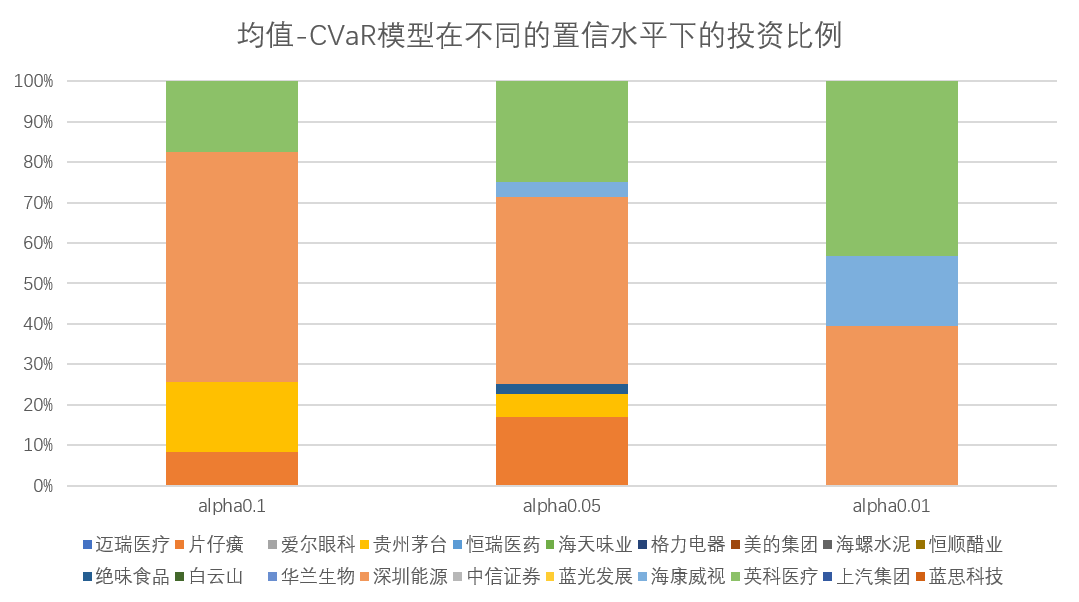
\includegraphics[width=0.85\textwidth]{均值-CVaR模型在不同的置信水平下的投资比例}
	\caption{均值-CVaR模型在不同的置信水平下的投资比例}
	\label{均值-CVaR模型在不同的置信水平下的投资比例}
\end{figure}
置信水平的选择使得均值-CVaR 模型相对于均值-方差模型在确立投资组合各资产权重配比方面有着更多的选择,更注重对风险的把控。另外,置信水平的选取对投资者的决策有着较大的影响。不同的置信度,会使投资者面临不同的权重配比。因此,投资者应根据自身的情况,选择适合自己风险偏好的置信水平来进行投资决策。
	\subsubsection{两模型汇总与分析}
	为了便于将两种模型进行对比,将均值-方差模型的3种情形的投资比例及对应的预期收益率、波动率(风险)、夏普比率,和均值-CVaR模型的3种置信水平的投资比例及对应的预期收益率、CVaR(风险)、条件夏普比率汇总如下表\ref{两模型投资组合比例及对应的收益风险汇总}.

% Table generated by Excel2LaTeX from sheet 'Sheet1'
\begin{table}[H]
	\centering
	\caption{两模型投资组合比例及对应的收益、风险汇总}
	\begin{tabular}{c|ccc|l|rrr}
		\toprule[1.5pt]
		\multicolumn{4}{c|}{\textbf{均值-方差模型}} & \multicolumn{4}{c}{\textbf{均值-CVaR模型}} \\
		\midrule[1.5pt]
		\textbf{名称} & \textbf{最小方差} & \textbf{最大预期收益} & \textbf{最大SharpRatio} & \multicolumn{1}{c|}{\textbf{名称}} & \multicolumn{1}{c}{\textbf{alpha0.1}} & \multicolumn{1}{c}{\textbf{alpha0.05}} & \multicolumn{1}{c}{\textbf{alpha0.01}} \\
		\midrule
		\textbf{迈瑞医疗} & \textbf{0.001} & \textbf{0} & \textbf{0} & \textbf{迈瑞医疗} & \textbf{0} & \textbf{0} & \textbf{0} \\
		\textbf{片仔癀} & \textbf{0} & \textbf{0} & \textbf{0.117} & \textbf{片仔癀} & \textbf{0.084} & \textbf{0.170} & \textbf{0} \\
		\textbf{爱尔眼科} & \textbf{0} & \textbf{0} & \textbf{0.008} & \textbf{爱尔眼科} & \textbf{0} & \textbf{0} & \textbf{0} \\
		\textbf{贵州茅台} & \textbf{0.066} & \textbf{0} & \textbf{0.178} & \textbf{贵州茅台} & \textbf{0.172} & \textbf{0.058} & \textbf{0} \\
		\textbf{恒瑞医药} & \textbf{0.114} & \textbf{0} & \textbf{0} & \textbf{恒瑞医药} & \textbf{0} & \textbf{0} & \textbf{0} \\
		\textbf{海天味业} & \textbf{0.046} & \textbf{0} & \textbf{0} & \textbf{海天味业} & \textbf{0} & \textbf{0} & \textbf{0} \\
		\textbf{格力电器} & \textbf{0.122} & \textbf{0} & \textbf{0} & \textbf{格力电器} & \textbf{0} & \textbf{0} & \textbf{0} \\
		\textbf{美的集团} & \textbf{0} & \textbf{0} & \textbf{0.077} & \textbf{美的集团} & \textbf{0} & \textbf{0} & \textbf{0} \\
		\textbf{海螺水泥} & \textbf{0.092} & \textbf{0} & \textbf{0} & \textbf{海螺水泥} & \textbf{0} & \textbf{0} & \textbf{0} \\
		\textbf{恒顺醋业} & \textbf{0} & \textbf{0} & \textbf{0} & \textbf{恒顺醋业} & \textbf{0} & \textbf{0} & \textbf{0} \\
		\textbf{绝味食品} & \textbf{0.053} & \textbf{0} & \textbf{0} & \textbf{绝味食品} & \textbf{0} & \textbf{0.024} & \textbf{0} \\
		\textbf{白云山} & \textbf{0.178} & \textbf{0} & \textbf{0} & \textbf{白云山} & \textbf{0} & \textbf{0} & \textbf{0} \\
		\textbf{华兰生物} & \textbf{0} & \textbf{0} & \textbf{0} & \textbf{华兰生物} & \textbf{0} & \textbf{0} & \textbf{0} \\
		\textbf{深圳能源} & \textbf{0.072} & \textbf{0} & \textbf{0.323} & \textbf{深圳能源} & \textbf{0.570} & \textbf{0.463} & \textbf{0.395} \\
		\textbf{中信证券} & \textbf{0} & \textbf{0} & \textbf{0} & \textbf{中信证券} & \textbf{0} & \textbf{0} & \textbf{0} \\
		\textbf{蓝光发展} & \textbf{0.185} & \textbf{0} & \textbf{0} & \textbf{蓝光发展} & \textbf{0} & \textbf{0} & \textbf{0} \\
		\textbf{海康威视} & \textbf{0.002} & \textbf{0} & \textbf{0.105} & \textbf{海康威视} & \textbf{0} & \textbf{0.037} & \textbf{0.173} \\
		\textbf{英科医疗} & \textbf{0.007} & \textbf{1} & \textbf{0.191} & \textbf{英科医疗} & \textbf{0.175} & \textbf{0.249} & \textbf{0.432} \\
		\textbf{上汽集团} & \textbf{0.062} & \textbf{0} & \textbf{0} & \textbf{上汽集团} & \textbf{0} & \textbf{0} & \textbf{0} \\
		\textbf{蓝思科技} & \textbf{0} & \textbf{0} & \textbf{0} & \textbf{蓝思科技} & \textbf{0} & \textbf{0} & \textbf{0} \\
		\midrule[1.5pt]
		\textbf{预期收益率} & \textbf{0.193} & \textbf{1.948} & \textbf{1.064} & \textbf{预期收益率} & \textbf{1.112} & \textbf{1.189} & \textbf{1.369} \\
		\textbf{预期波动率} & \textbf{0.176} & \textbf{0.778} & \textbf{0.280} & \textbf{CVaR} & \textbf{0.030} & \textbf{0.042} & \textbf{0.067} \\
		\textbf{SharpRatio} & \textbf{1.095} & \textbf{2.503} & \textbf{3.799} & \textbf{条件SharpRatio} & \textbf{37.264} & \textbf{28.026} & \textbf{20.308} \\
		\bottomrule[1.5pt]
	\end{tabular}%
	\label{两模型投资组合比例及对应的收益风险汇总}%
\end{table}%

为了更好地了解各种权重比例下的预期收益,按以上6种权重进行模拟投资,对一年内每天的收益进行累积,并增加一种等权重投资的对照组,绘制收益曲线如图\ref{两模型求得的不同权重下的收益曲线},其中Portfolio\_EW为等权重投资对照组。
		\begin{figure}[H]
	\centering
	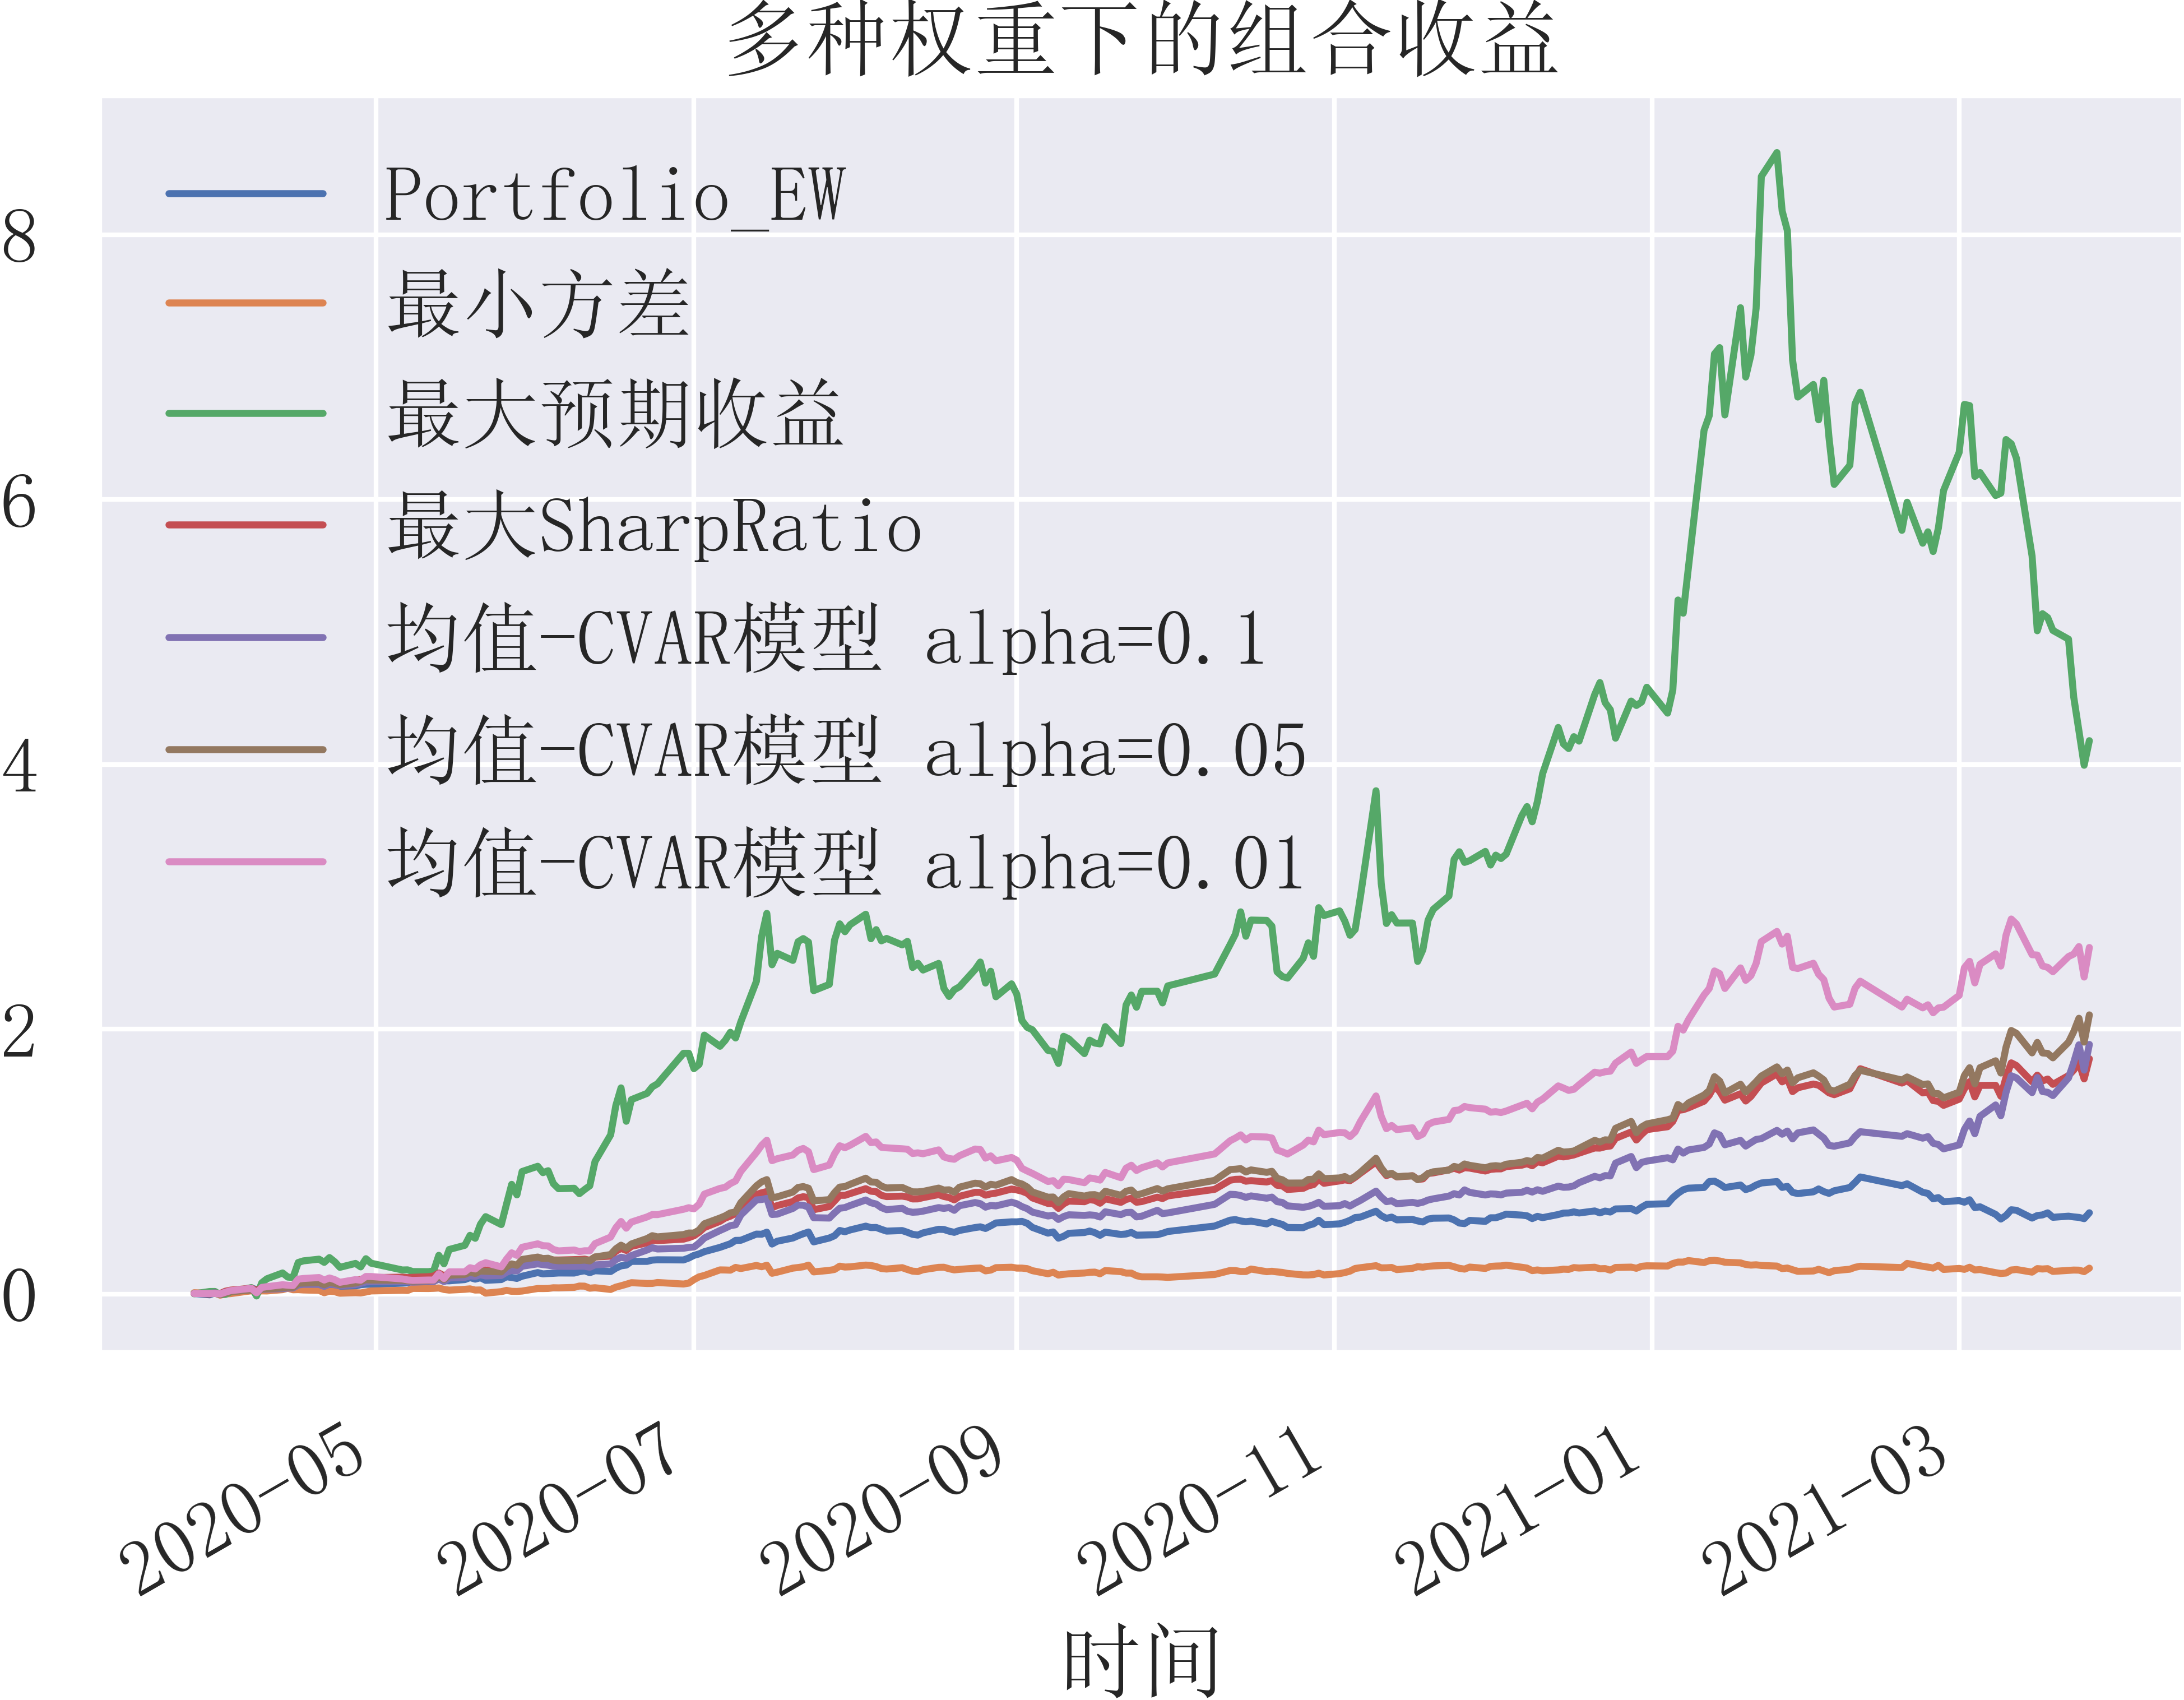
\includegraphics[width=0.85\textwidth]{最小方差最大预期收益最大SharpRatio_CVAR}
	\caption{两模型求得的不同权重下的收益曲线}
	\label{两模型求得的不同权重下的收益曲线}
\end{figure}
可见,最大预期收益的曲线与其他曲线相差较大,排除最大预期收益的曲线,最终收益率由高到低分别是
置信水平为99\%、95\%、90\%的均值-CVaR曲线,以及最大夏普比率、最小方差的均值-方差模型曲线。并且可以看到,除最小方差模型外,其他模型的收益率曲线都远超等权重投资时的曲线,说明我们的模型达到了很好的效果,兼顾了收益最大化和风险最小化。

同时,均值-CVaR模型加入置信水平的选择,而使得在投资组合优化过程中,强化了风险和收益间相互关系,也让不同风险偏好的投资者有了更合理的模型选择。
	
	\section{模型的评价}
	本文以前人的理论为基础,建立了Markowitz 均值-方差模型,和均值-CVaR模型,并依照此模型进行了投资组合优化的分析。本文作出以下评价:
	
	第一,对于投资组合的优化,好的风险度量对于投资组合各资产的权重配比有着不可忽略的影响。不同的风险度量方法会得到不同的优化结果。在这些方法中,均值-方差模型是最基础的数量化方法;CVaR 方法给出了超额风险的具体数值,由于CVaR 给出了超过极端损失额的条件均值\upcite{houJiYuShangHeCVaRDeDuoMuBiaoTouZiZuHeMoXingJiShiZhengYanJiu2021},使得该类方法可以向投资者提供更简洁、更直观的风险信息。
	
	第二,利用因子分析对20只股票数据进行分析,能给予各个指标更准确的权重,减少主观赋予权重的随机性,股票在各个因子上的得分也准确地反映了股票在某个方面的指标健康情况。同时,通过特定权重计算得到的综合因子得分,能实现对多个股票的横向排序比较。
	
	第三,本文对样本股票进行了正态性检验。检验表明股票的收益率序列呈现一定程度上的左偏或右偏,部分股票更是具有金融时间序列典型的尖峰厚尾、波动集聚的特征。这说明股票收益率是不服从正态分布的,采用方差-协方差的方法是不合适的。所以本文采用了历史模拟法规避了正态分布假设所造成的误差。
	
	第四,均值-方差模型和均值-CVaR投资组合优化模型可转化为一个线性规划求解模型,求解结果构成了各自的有效前沿。对均值-CVaR模型同时加入置信水平的选择,而使得在投资组合优化过程中,强化了风险和收益间相互关系,也让不同风险偏好的投资者有了更合理的模型选择。

	
	在本文的建模过程中,还存在一些问题没有得到解决,尚需进一步地研究:
	
	第一,本文在建模过程中并没有加入过多的限制条件,比如是否卖空,有无交易费用等实际投资操作中无法忽略的因素。事实上,确定一个有效合理的投资组合是一个非常复杂的决策过程,需要综合考虑投资者的资金限额、交易费用、是否卖空、持有期长短、无风险资产的存在、通货膨胀以及期望收益率目标是否合理等各种因素,加入各种约束或者参数\upcite{liDaiYueShuDeTouZiZuHeYouHuaWenTiDeGaoXiaoJuBuSouSuoYanJiu2019a},构建更加复杂的投资模型,方能得到最优的投资组合。
	

	第二,市场真实的波动情况被掩盖。本文采用历史模拟法进行实证,由于历史模拟法是一种统计估计的方法,完全依赖于样本数据,在市场有效性的假设下进行计算。但由于选取的时间较短,历史模拟法的误差目前尚无法估计。


	%\section{参考文献}
	%\addcontentsline{toc}{section}{参考文献}
	%\bibliographystyle{bib/gbt7714-2005}
	\bibliographystyle{gbt7714-numerical}
	%\bibliographystyle{unsrt}
	%\bibliographystyle{IEEEtran}
	\bibliography{bib/ref.bib}
	
	\newpage
	%附录
	\begin{appendices}
		\section{代码}
		\lstinputlisting[language=python]{code/py/test1.py}
	
	\end{appendices}
	
\end{document} 